%% 使用 zhbook 文档类生成中文科技书籍的示例文档
%%
%% 作者:陈渝 向勇,yuchen@tsinghua.edu.cn
%% 项目主页: https://github.com/chyyuu/simple_os_book
%%
%% 本样例文档中用到了胡海星提供的zhbook 文档类生成中文文档,在此对他表示感谢。
%%
\documentclass{zhbook}


 \usepackage{listings}
 \usepackage{xcolor}
 \lstset{
   %行号
   numbers=left,
   %背景框
   framexleftmargin=10mm,
   frame=none,
   %背景色
   %backgroundcolor=\color[rgb]{1,1,0.76},
   backgroundcolor=\color[RGB]{245,245,244},
   %样式
   keywordstyle=\bf\color{blue},
   identifierstyle=\bf,
   numberstyle=\color[RGB]{0,192,192},
   commentstyle=\it\color[RGB]{0,96,96},
   stringstyle=\rmfamily\slshape\color[RGB]{128,0,0},
   %显示空格
   showstringspaces=false
 }
 
 % \dangericon 表示警告的图标
 \font\manfnt=manfnt
 \newcommand*{\dangericon}{\manfnt\char127}
 
 % note 环境表示需特别注意的内容
 \newenvironment{note}
 {\vskip1.5ex\par\noindent\llap{\dangericon\hskip2mm}\textbf{注意:}}
 {\vskip1.5ex}
 
%%%%%%%%%%%%%%%%%%%%%%%%%%%%%%%%%%%%%%%%%%%%%%%%%%%%%%%%%%%%%%%%%%%%%%%%%%%%%%%
% 设置论文的中文封面

% 论文标题,不可换行
\title{操作系统的简单实现与基本原理 \newline --- 基于ucore OS + RISC-V}
\englishtitle{Simple Implementation and Basic Principle of Operating Systems \\ --- based on ucore OS + RISC-V}
% 如果论文标题过长,可以分两行,第一行用\titlea{}定义,第二行用\titleb{}定义,将上面的\title{}注释掉
%\titlea{操作系统的基本原理与简单实现}
%\titleb{--基于ucore OS + RISC-V}

% 书籍作者姓名
\author{陈渝 \ \ 向勇}
% 书籍出版社
\publisher{}
%\publishercity{北\hspace{1.5em}京}
\date{二〇一八年}

%%%%%%%%%%%%%%%%%%%%%%%%%%%%%%%%%%%%%%%%%%%%%%%%%%%%%%%%%%%%%%%%%%%%%%%%%%%%%%%
\begin{document}

%%%%%%%%%%%%%%%%%%%%%%%%%%%%%%%%%%%%%%%%%%%%%%%%%%%%%%%%%%%%%%%%%%%%%%%%%%%%%%%
\, 
% 制作中文封面
\maketitle
% 制作英文封面
% \makeenglishtitle

%%%%%%%%%%%%%%%%%%%%%%%%%%%%%%%%%%%%%%%%%%%%%%%%%%%%%%%%%%%%%%%%%%%%%%%%%%%%%%%
% 开始前言部分
\frontmatter

%\begin{abstract}

本书想讲解一个问题:操作系统是如何帮助应用程序在硬件上运行的。

操作系统课是计算机科学与技术专业的一门重要的专业基础课,但仅仅介绍操作系统这个单一知识是不够的。传统操作系统课程的一个重要问题,就是把操作系统进行高度的抽象、割裂,使得学生在学习操作系统时,先从各种相对孤立的抽象概念原理为主的知识点进行学习,缺少对“为什么”,“具体如何做的”等问题的深刻和综合的理解。学完之后,可能还存在对一个完整操作系统的全貌缺少把握,对操作系统中各个关键组成部分的联系缺少认识,不能站在计算机系统的角度来看待操作系统等问题。

虽然学生已经学习了算法与数据结构、编译原理、计算机原理、汇编程序设计,并从不同的角度对计算机系统进行了了解。当学生在面临一个具体问题的时候,比如理解一个显示”hello worlod!“的C语言程序是如何在一个具体硬件上完成这个字符串的显示时,是需要综合考虑到这个C程序是如何被编译器变成执行程序,被操作系统加载执行,如何被操作系统通过文件的方式来驱动相应的外设显示字符串等。如果学生能够理解这些具体的过程,并能进一步归纳总结,形成自己理解的概念,原理,规律,方法等,那么对站在计算机系统来看操作系统,就会有更深入的掌握了。

操作系统是一个软件,讲述一个操作系统的总体架构,模块划分,渐进扩展和具体实现会加深对操作系统原理的理解。操作系统离不开硬件的支持,如果缺少对硬件的理解,那么操作系统在硬件内部的运行过程就是一个黑盒子,使得很难深刻理解操作性与硬件的配合所提供的强大功能。操作系统的主体一般是通过高级语言实现的,并由编译器生成机器码在硬件上执行,如果不理解高级语言与机器码的对应关系,不理解编译器生成的执行程序的内容,那么对于操作系统如何加载运行程序,如何进行运行程序的切换等就缺少综合的考虑。


为此,本书的讲述方式是从具体实践到概括抽象,从操作系统需要应对的需求出发,从简单的IO输出支持到最后的shell运行支持,逐步实现和扩展操作系统的能力,并逐步完成对操作系统概念、定义、原理、算法等的归纳总结。在讲解操作系统的基本原理之前,将介绍在基于RISC-V CPU的计算机系统上用C语言设计实现一个简单操作系统ucore OS,分析此操作系统在一个具体的计算机硬件系统上执行过程。并对编译器、计算机组成原理、操作系统的相互关系进行系统的介绍。使得抽象的操作系统概念原理能与具体的操作系统设计实现能够相互印证,相互补充。为读者对操作系统的学习和掌握打下坚实的基础。希望通过本书的介绍,可以使读者全面地了解和掌握操作系统的目标、功能、机制、策略、基本原理与算法等的思路,并能够领会操作系统的功能和实现过程。

本书的内容展开是围绕着一个操作系统从无到有的过程来讲解的,并配合计算机组成原理和编译原理方面的补充。这在某种程度上也反映了操作系统和计算机硬件组成的发展历史。具体而言,本书内容包括:操作系统概述;操作系统的启动;操作系统与硬件进行的基本交互;操作系统对物理内存的管理;操作系统对CPU的分时复用;可在用户态运行的程序;虚拟内存的设计与实现;调度算法;同步和通信;死锁;进程间通信;文件系统。

%\end{abstract}
%%%%%%%%%%%%%%%%%%%%%%%%%%%%%%%%%%%%%%%%%%%%%%%%%%%%%%%%%%%%%%%%%%%%%%%%%%%%%%%
% 论文的前言,应放在目录之前,中英文摘要之后
%
\begin{preface}

对于在校的学生和已经参加工作的工程师而言,能否以较小的时间和精力比较全面地了解操作系统呢?陆游老夫子说过“纸上得来终觉浅,绝知此事要躬行”,也许在了解基本的操作系统概念和原理基础上,通过实际动手来一步一步分析、设计和实现一个微型化的操作系统,会发现操作系统原来如此,并会发现操作系统的概念原理与实际实现之间有紧密的联系和巨大的差异。

早期开放开源的UNIX操作系统和MIT教授 Frans Kaashoek 等基于UNIX v6设计的xv6操作系统给了我们启发:对一个计算机专业的本科生而言,设计实现一个操作系统有挑战但是可行!但x86相对封闭且复杂和有一定历史包袱的CPU硬件接口给OS学习带来了一定的挑战。1980年前后,UC Berkeley的Dave Patterson主导了Berkeley RISC项目并设计了其第一代的处理器RISC I,并在2014年发展到了开放且开源的第五代指令集架构RISC-V。本书想进行这样的教学尝试,以操作系统基本原理为教学引导,以简洁的RISC-V CPU为底层硬件基础,以C语言为主,设计并实现一个微型但全面的“麻雀”操作系统—ucore。期望能够采用简化的计算机硬件为基础,以操作系统的基本概念和核心原理为实践指导,逐步解析操作系统各种知识点和对应的实验,做到有“理”可循和有“码”可查,最终让读者了解和掌握操作系统的原理、设计与实现。

\paragraph{读者要具备的背景知识}
操作系统课程一般安排在本科大二或大三上课。这其中的原因是希望学生已经完成了算法与数据结构、编译原理、计算机原理、汇编程序设计等课程的学习。如果读者没有完成上述课程的学习,本书希望读者能够有一个Linux系统可以用来做实验,这需要有基本的Linux的使用操作能力,另外有基本的基于C语言的算法和数据结构编程能力,最后就是对计算机的基本原理,比如CPU,内存在功能上的体现有基本的了解。

本书希望通过设计实现操作系统来更好地理解操作系统原理和概念。设计实现操作系统其实就是设计实现一个可以管理CPU、内存和各种外设,并管理和服务应用软件的系统软件。为此还是需要先了解一些基本的计算机原理和编程的知识。本书的例子和描述需要读者学习过计算机原理课程、程序设计课程,掌握C语言编程(了解指针等的编程)。如需完成基于RISCore实验,则对基于RISC-V的体系结构有一定的了解,大致了解RISC-V的汇编语言。

\paragraph{本书结构}

本书的知识内容由XXX章组成,旨在通过分析操作系统的具体设计与运行来阐述操作系统的核心概念。

\paragraph{操作系统初级阶段}	

\begin{itemize}
	\item
	\subparagraph{绪论} 这一章首先介绍了操作系统的历史,从中了解操作系统与应用需求和计算机硬件是相互促进,逐步发展起来的。然后通过分析"hello world"这个简单程序的生命周期,介绍编译、操作系统、计算机原理等的相关知识和在计算机系统层面上的相互关。并进一步描述了ucore-os操作系统的功能和总体结构,以及操作系统的主要概念和主题。最后介绍了操作系统所依赖的计算机硬件架构的主要概念和一个具体的RISC-V CPU。

	\item
	\subparagraph{启动操作系统}本章介绍
	\item
	\subparagraph{内存管理管理}本章介绍
	\item
	\subparagraph{并发管理}本章介绍
	\item
	\subparagraph{异常与中断管理}本章介绍
	\item
	\subparagraph{特权级管理}本章介绍
\end{itemize}

\paragraph{操作系统中级阶段}
\begin{itemize}
	\item
	\subparagraph{虚拟内存管理}本章介绍	
	\item
	\subparagraph{进程管理}本章介绍
	\item
	\subparagraph{处理器调度}本章介绍	
	\item
	\subparagraph{同步互斥管理}本章介绍
	\item
	\subparagraph{死锁}本章介绍					
	\item
	\subparagraph{文件系统管理}本章介绍		
\end{itemize}	

\paragraph{操作系统高级阶段}
\begin{itemize}
	\item
	\subparagraph{64位CPU支持}本章介绍		
	\item
	\subparagraph{多核/SMP管理与调度}本章介绍	
	\item
	\subparagraph{同步互斥进阶}本章介绍	
	\item
	\subparagraph{日志文件系统}本章介绍		
	\item
	\subparagraph{虚拟文件系统}本章介绍		
	\item
	\subparagraph{基于rust语言的OS设计}本章介绍	
	\item
	\subparagraph{高并发度OS设计}本章介绍		
\end{itemize}

\vspace{1cm}
\begin{flushright}
陈渝 \ 向勇\\
2018年夏于清华园
\end{flushright}

\end{preface}

%%%%%%%%%%%%%%%%%%%%%%%%%%%%%%%%%%%%%%%%%%%%%%%%%%%%%%%%%%%%%%%%%%%%%%%%%%%%%%%
% 生成论文目次
\tableofcontents

%%%%%%%%%%%%%%%%%%%%%%%%%%%%%%%%%%%%%%%%%%%%%%%%%%%%%%%%%%%%%%%%%%%%%%%%%%%%%%%
% 生成插图清单。如无需插图清单则可注释掉下述语句。
\listoffigures

%%%%%%%%%%%%%%%%%%%%%%%%%%%%%%%%%%%%%%%%%%%%%%%%%%%%%%%%%%%%%%%%%%%%%%%%%%%%%%%
% 生成附表清单。如无需附表清单则可注释掉下述语句。
\listoftables

%%%%%%%%%%%%%%%%%%%%%%%%%%%%%%%%%%%%%%%%%%%%%%%%%%%%%%%%%%%%%%%%%%%%%%%%%%%%%%%
% 开始正文部分
\mainmatter

%%%%%%%%%%%%%%%%%%%%%%%%%%%%%%%%%%%%%%%%%%%%%%%%%%%%%%%%%%%%%%%%%%%%%%%%%%%%%%%

\chapter{绪论}\label{ch_intro}

\section{本章概要}

\paragraph{一句话描述}

用”hello world“程序作为向导,站在一万米的高空看操作系统的发展和特征!

\paragraph{概述}

计算机系统是由硬件和系统软件((主要是操作系统)组成的,它们共同工作来运行应用程序。纵观计算机相对很短的发展史,虽然计算机系统的具体实现方式不断变化,越来越复杂,但是计算机系统内在的概念保持相对稳定。所有计算机系统在原理上基于天才的图灵机,在设计上基于伟大的冯诺依曼架构,有相似的硬件和软件组件,它们执行着相似的功能。本章主要以操作系统为主来理解计算机系统如何支持一个C语言编写的”hello world“程序完成它的功能。

这里先简要介绍一下操作系统的历史,然后将从一个C语言编写的”hello world“程序开始,讲述操作系统和涉及到的编译,计算机原理等的一些基础知识,以及对操作系统的基本架构和用于本书的ucore教学操作系统做一个初步介绍。在其中穿插介绍操作系统的基本概念、操作系统抽象以及操作系统的特征。

%
%本书希望通过设计实现操作系统来更好地理解操作系统原理和概念。设计实现操作系统其实就是设计实现一个可以管理CPU、内存和各种外设,并管理和服务应用软件的系统软件。为此还是需要先了解一些基本的计算机原理和编程的知识。本书的例子和描述需要读者学习过计算机原理课程、程序设计课程,掌握C语言编程(了解指针等的编程)。如需完成基于RISCore实验,则对基于RISC-V的体系结构有一定的了解,大致了解RISC-V的汇编语言。

%\section{预备知识}
本书希望通过设计实现操作系统来更好地理解操作系统原理和概念。设计实现操作系统其实就是设计实现一个可以管理CPU、内存和各种外设,并管理和服务应用软件的系统软件。为此还是需要先了解一些基本的计算机原理和编程的知识。本书的例子和描述需要读者学习过计算机原理课程、程序设计课程,掌握C语言编程(了解指针等的编程)。如需完成基于RISC-V的ucore实验,则对基于RISC-V的体系结构有一定的了解,大致了解RISC-V的汇编语言。

\section{初步了解操作系统}

我们可以把软件分成应用软件和系统软件。所谓应用软件,即完成某种特定应用功能的软件,比如写文档的office软件,玩游戏的游戏软件等。所谓系统软件,即完成系统功能的软件,这里的系统功能相对与特定应用功能而言,更加底层和通用,比如编译器,C运行时库,操作系统等。而对于系统软件,我们又可以分为系统应用((编译器,C运行时库等)和操作系统。这里把操作系统单独分出来,是由于操作系统直接管理了硬件,所有的应用都需要操作系统的支持,才能正常工作。

操作系统其实是一个相比较复杂的系统软件,直接管理计算机硬件和各种外设,以及给应用软件提供帮助。这样描述还太简单了一些,我们可对其进一步描述:操作系统是一个可以管理CPU、内存和各种外设,并管理和服务应用软件的软件。为了完成这些工作,操作系统需要知道如何与硬件打交道,如何更好地服务好应用软件。

\subsection{操作系统历史}

在大众的眼中,操作系统就是他们的手机/终端上的软件系统,包括各种应用程序集合,但在历史上,操作系统也是从无到有地逐步发展起来的。操作系统主要完成对硬件控制和对应用程序的服务所必需的功能,操作系统的历史与计算机发展的历史密不可分。操作系统的内涵和功能随着历史的发展也在一直变化,改进中,在今天,没有图形界面和各种文件浏览器已经不能称为一个操作系统了。

\subsubsection{三叶虫时代}

计算机在最开始出现的时候是没有操作系统的。启动,扳开关,装卡片/纸带等比较辛苦的工作都是计算机操作员(Operator)或者用户自己完成。操作员/用户带着记录有程序和数据的卡片(punch card)或打孔纸带去操作机器。装好卡片/纸带后,启动卡片/纸带阅读器,让计算机把程序和数据读入计算机机的内存中后,计算机就开始工作,并把结果也输出到卡片/纸带或显示屏上,最后程序停止。

由于人的操作效率太低,计算机的机时宝贵,所以就引入监控程序(Monitor)辅助完成输入,输出,加载,运行程序等工作,这是现代操作系统的起源。一般情况下,计算机每次只能执行一个任务,CPU大部分时间都在等待人的缓慢操作。

\subsubsection{恐龙时代}

早期的操作系统非常多样化,专用化,生产商生产出针对各自硬件的专用操作系统,大部分用汇编语言编写,这导致操作系统的进化比较缓慢,但进化再持续。在1964年,IBM公司开发了面向System/360系列机器的统一可兼容的操作系统——OS/360。OS/360是一种批处理操作系统。为了能充分地利用计算机系统,应尽量使该系统连续运行,减少空闲时间,所以批处理操作系统把一批作业(古老的术语,可理解为现在的程序)以脱机方式输入到磁带上,并使这批作业能一个接一个地连续处理:1)将磁带上的一个作业装入内存;2)并把运行控制权交给该作业;3)当该作业处理完成后,把控制权交还给操作系统;4)重复1-3的步骤。

批处理操作系统分为单道批处理系统和多道批处理系统。单道批处理操作系统只能管理内存中的一个(道)作业,无法充分利用计算机系统中的所有资源,致使系统整体性能较差。多道批处理操作系统能管理内存中的多个(道)作业,可比较充分地利用计算机系统中的所有资源,提升系统整体性能。二者的共同特点是人机交互性差,这对修改和调试程序很不方便。

\subsubsection{哺乳动物时代}

20世纪60年代末,提高人机交互方式的分时操作系统越来越展露头角。分时是指多个用户和多个程序以很小的时间间隔来共享使用同一台计算机上的CPU和其他硬件/软件资源。1964年由贝尔实验室、麻省理工学院及美国通用电气公司所共同参与研发目标远大的MULTICS(MULTiplexed Information and Computing System)操作系统,MULTICS是一套安装在大型主机上多人多任务的操作系统。 MULTICS以兼容分时系统(CTSS)做基础,建置在美国通用电力公司的大型机GE-645,目标是连接1000部终端机,支持300的用户同时上线。因MULTICS项目的工作进度过于缓慢,1969年AT\&T的 Bell 实验室从MULTICS 研发中撤出。但贝尔实验室的两位软件工程师 Thompson 与 Ritchie借鉴了一些重要的Multics理念,以C语言为基础,发展出UNIX操作操作系统。UNIX操作系统的早期版本是完全免费的,可以轻易获得并随意修改,所以它得到了广泛的接受。后来,它成为开发小型机操作系统的起点。由于早期的广泛应用,它已经成为的分时操作系统的典范。

\subsubsection{古猿人时代}

20世纪70年代,微型处理器的发展使计算机的应用普及至中小企及个人爱好者,推动了个人计算机(Personal Computer)的发展,也进一步推动了面向个人使用的操作系统的出现。其代表是由微软公司中在20世纪80年代为个人计算机开发的DOS/Windows操作系统,其特点是简单易用,特别是基于Windows操作系统的GUI界面,极大地简化了一般用户使用计算机的难度,使得计算机得到了快速的普及。这里需要注意的是,第一个带GUI界面的个人计算机原型起源于伟大却又让人扼腕叹息的施乐帕洛阿图研究中心PARC(Palo Alto Research Center),PARC研发出的带有图标、弹出式菜单和重叠窗口的GUI(Graphical User Interface),可利用鼠标的点击动作来进行操控,这是当今我们所使用的GUI系统的基础。

\subsubsection{智人时代}

智人时代的操作系统的代表是Linux操作系统内核(Linux kernel),它覆盖了工业控制、物联网、移动终端、桌面计算机、服务器、数据中心到超级计算机的各个领域。其中面向移动终端的Android操作系统基于Linux kernel,已成为21世纪个人终端操作系统的代表之一,Linux kernel在巨型机到数据中心服务器操作系统中也占据了统治地位。

1991年8 月,芬兰学生 Linus Torvalds(中文名:林纳斯·托瓦兹)在 comp.os.minix 新闻组贴上了以下这段话: 

"你好,所有使用 minix 的人 -我正在为 386 ( 486 ) AT 做一个免费的操作系统 ( 只是为了爱好 )......"

而他所说的"爱好″就变成我们今天知道的 Linux kernel。 Linus Torvalds采用了GPL版权协议,通过Internet发布了 Linux kernel的源代码。在Internet的日渐盛行以及 Linux 开放自由的GPL版权之下,吸引了无数计算机Hacker和公司投入开发、改善Linux kernel,使得 Linux kernel的功能日见强大并被广泛使用。 

\subsubsection{神人时代}

当前,大数据、人工智能、机器学习、高速网络、AR/VR对操作系统等系统软件带来了新的挑战。如何有效支持和利用这些技术是未来操作系统的方向。\emph{注:面向此时代的操作系统目前还未出现。}



\subsection{hello world漫游}

本节希望通过显示“hello world!”的应用程序来感受操作系统的功能和特征。一般应用程序都希望能够完成接受输入、显示输出、保存结果、定时处理、程序执行切换等基本功能,而这些功能都是在操作系统的帮助下完成的。

\subsubsection{智人时代下的"hello world!"}

智人时代的典型操作系统是Linux和Windows。Linux和Windows都非常强大,在这两个操作系统上编写和执行“显示“hello world!”的各种应用程序很容易,容易到你都感觉不到操作系统的存在。相对而言,Linux可以看到它的源代码,用到的各种工具和操作相对也原始一些,可以让读者与操作系统的距离感更近一些,对于理解操作系统的实现会有很大帮助,所以我们以Linux作为我们的实验环境。
接下来的五个小实验,分别基于不同的需求完成对“hello world!”的显示:
\begin{itemize}
	\item 在显示器上直接显示字符串;
	\item 通过定时器在显示器上定时显示字符串;
	\item 把字符串“显示”到磁盘上永久保存;
	\item 可根据键盘输入改变字符串的显示内容;
	\item 定时显示程序和交互显示程序一起执行。
\end{itemize}

通过这些实验,我们可以看到操作系统的一个重要功能是给应用程序提供了便捷的访问服务,应用程序只需发出要求,比如显示字符串、保存文件、定时唤醒、接收输入等,操作系统就可以帮助它完成;另外还有一些很重要的看不见的管理服务,比如给应用程序提供执行环境,切换应用程序,回收应用程序占用的资源等,这些就不能直接地感受到了。而对于硬件,比如显示器、定时器、磁盘、键盘等各种外设,操作系统都把它们很好地管理起来,提供了外设管理服务,使得我们的应用程序很方便地通过一些简单的AP就可以访问这些外设,而不需要关注外设的复杂控制细节。


\begin{note} 
下面的实验环境是基于ubuntu-16.04 x86-64环境,虽然CPU是x86-64,当下面的实验完全没有涉及到x86-64的细节,所以在这里就直接忽视让操作系统和应用正常运行的这个不可或缺的一个或多个CPU和其他不相关的硬件细节。
\end{note}

\paragraph{显示"hello world!"}
让我们通过智人时代的操作系统Linux来感受一下显示一个字符串的过程。假定读者建立了Linux实验环境(参见\ref{setuplinux}),对C语言有一定的了解,所以可以写出如下的代码 helloworld.c:
\begin{lstlisting}[language={C}]
void main(void)
{
  puts("hello world!");
}
\end{lstlisting}

并在Linux环境中的shell界面下,执行gcc编译命令,把helloworld.c转换成执行程序helloworld:

\begin{lstlisting}[language={bash}]
$ gcc -o helloworld helloworld.c
\end{lstlisting}

在shell界面下,在生成执行程序helloworld的目录下执行此程序,可以看到程序显示出了“hello world!”:
%\begin{lstlisting}[language={bash},numbers=none]
\begin{lstlisting}[language={bash}]
	  $ helloworld
	  hello world!
\end{lstlisting}


只要读者会基本编程,对于上面的输出结果,应该不会感到陌生。但读者对具体的执行过程了解吗?Linux操作系统和它用的x86计算机硬件太复杂,如果要详细分析和解释上面示例的两行显示背后的具体执行过程的细节,我们可以写出一本超过1000页的大部头。考虑到读者时间有限,下面我们将站在操作系统的角度来简单理解一下这个helloworld程序的执行过程。

%上面的操作过程,需要与人交互的有两个外设,一个是键盘,一个是显示器。首先,你看到的是\$符号,这是一个正在运行的程序shell的人机交互界面。在你没敲字符的时候,\textbf{shell处于睡觉状态}。当你通过键盘敲入“g”和后续的多个字符的时候,首先是操作系统收到键盘发出的字符,然后通知shell,有字符来了!shell本来在睡觉,被操作系统唤醒后,接收字符,并发出显示字符的请求给操作系统。操作系统收到shell的请求后,把字符显示到显示器上,然后通知shell完成显示字符任务了。当shell程序收到回车字符的时候,就开始把整个字符串看成是一个命令,解析完此命令后,并告知操作系统,继续请操作系统帮忙执行另外一个程序gcc来完成整个编译过程。操作系统为此需要创建一个让gcc可以正常工作的执行空间,并启动gcc程序,让它能够完成整个编译过程。gcc于是开始干活,首先请操作系统把helloworl操作系统d.c这个文件从磁盘上读到内存中,gcc对内存中的helloworld.c的内容进行编译,生成helloworld执行程序,但此时这个程序还在内存中。于是gcc继续请操作系统帮忙,把这个helloworld执行程序写到磁盘上。当你看到第二个\$符号出现的时候,表示gcc的工作完成了。

%上面的helloworld执行程序需要用到一个个外设:显示器。dang\$上继续敲如字符串"hello world!",并回车。类似上面的描述,这次shell程序会请求操作系统来执行helloworld这个程序。操作系统为此需要创建一个让helloworld程序可以正常工作的执行空间,并启动helloworld程序。helloworld的执行工作就是显示字符串“hello world!”。为此,它像shell一样,给操作系统发出显示字符串的请求。操作系统收到显示字符串的请求后,把字符串显示到屏幕上。至此,上面示例中三行显示的背后执行过程就简单描述完毕。

上面的helloworld执行程序需要用到一个外设:显示器。当你在shell的\$提示符后继续敲如字符串"hello world!"并回车,shell解析此命令,分析出你是要执行helloworld这个程序,于是会请求操作系统来执行helloworld这个程序。操作系统为此需要创建一个让helloworld程序可以正常工作的执行环境(比如分配内存放代码和数据,提供CPU用于执行等),并启动helloworld程序。此时shell程序要让位helloworld程序执行,为此操作系统还要完成一个执行上下文切换的过程,让helloworld能够占用CPU来执行。完成切换后,helloworld程序才真正开始执行。

helloworld的执行工作就是显示字符串“hello world!”。为此,它像shell一样,给操作系统发出显示字符串的请求。操作系统收到显示字符串的请求后,直接控制显卡这个设备,通过显卡把字符显示到显示器上,然后通知shell完成显示字符任务了。helloworld程序执行完毕后,操作系统还要把之前分配给helloworld的执行环境给收回,用于其他程序的执行。至此,上面示例中两行行显示的背后执行过程就简单描述完毕。

\begin{note} 
操作系统其实也没有直接控制显示器,而是通过控制显卡,让显卡访问显示器上显示信息的。
\end{note}

\paragraph{每秒定时显示"hello world!"}
如果要每秒定时显示字符串,很显然需要时钟外设来帮助实现定时。添加一点代码形成timing-helloworld.c,就可以实现定时显示helloworld了。
\begin{lstlisting}[language={C}]
void main(void)
{
  while(1) {
    sleep(1);
    puts("hello world!");
  }
}
\end{lstlisting}

在Linux环境中,执行gcc编译命令,把timing-helloworld.c转换成执行程序timing-helloworld,并执行生成的执行程序timing-helloworld:
\begin{lstlisting}[language={bash}]
	$ gcc -o timing-helloworld timing-helloworld.c
	$ timing-helloworld
	hello world!
	hello world!
	......
\end{lstlisting}

可以看到,当执行timing-helloworld程序时,屏幕上会每隔一秒重复显示“helloworld”。新增加的sleep函数完成了等待一秒并恢复执行的功能。其实这个功能也是靠藏在后面的操作系统帮忙完成的。当timing-hellworld执行sleep(1)函数时,它向操作系统发出了一个请求,要求操作系统先让它睡觉,且让操作系统帮它设个1秒到期的闹钟(更正式的说法是定时器)。于是操作系统先把timing-helloworld设置为睡眠状态,且对时钟外设做好配置,让它1秒中后产生一个中断,通知操作系统到点了。操作系统做完这两件事后,就忙自己的其他事情并安排调度其他程序运行。过了1秒后,时钟外设产生了一个中断,通知操作系统到点了,操作系统响应这个中断,并记得timing-hellworld需要被唤醒并继续运行,于是就把timing-hellworld唤醒,并让它继续运行。这样,timing-hellworld就开始每隔1秒显示字符串了。

\paragraph{把"hello world!"字符串存到磁盘上}

如果要把显示字符串长久保存下来,很显然需要磁盘外设来帮助实现长期存储的功能。添加一点代码形成file-helloworld.c,就可以实现把字符串保存到磁盘上了。

\begin{lstlisting}[language={C}]
#include <stdio.h>
void main(void){
  FILE *fp;
  fp = fopen("file-helloworld.txt", "w");
  fputs("hello world!",fp);
  fclose(fp);
}
\end{lstlisting}

在Linux环境中,执行gcc编译命令,把file-helloworld.c转换成执行程序file-helloworld,并执行生成的执行程序file-helloworld:
\begin{lstlisting}[language={bash}]
	$ gcc -o file-helloworld file-helloworld.c
	$ file-helloworld
	$ more file-helloworld.txt
	hello world!	
\end{lstlisting}

可以看到,当执行file-helloworld程序时,当前目录下多了一个文件file-helloworld.txt,通过more命令,可以看到file-helloworld.txt文件的内容就是我们需要保存的字符串"hello world!"。这里我们可以看到通过操作系统,应用程序可用文件的形式方便地把字符串存储到磁盘上,而没有关注磁盘磁盘的细节。当执行程序file-helloworld的时候,操作系统做了啥呢?首先,当file-helloworld执行fopen函数时,会请求操作系统在当前目录下创建一个可写的文件file-helloworld.txt。于是操作系统会定位到当前目录在磁盘上的位置,并在此目录下添加一个文件,此时的文件内容为空。然后当file-helloworld执行fput函数时,会请求操作系统把"hello world!"这个内容写到file-helloworld.txt文件中。于是操作系统定位到file-helloworld.txt文件在磁盘中的位置,给这个文件分配空闲磁盘扇区空间用于存放文件内容,再把位于内存中的字符串"hello world!"以磁盘块为单位,写入到文件内容对应的磁盘扇区中。



\paragraph{交互式显示"hello world!"}

上面三个小实验缺少了一点与人的交互。比如,如果我敲了一个名字“human”,程序就能显示"human, hello world!"。让程序能接收输入,那还需要一个外设:键盘。通过键盘,程序就可以得到人的输入了。getchar-helloworld.c的代码如下:

\begin{lstlisting}[language={C}]
void main(void)
{
  char name[100];
  int i=0;
  while((name[i] = getchar())!='\n' && i<80)
        i++ ;
  name[i]=0;
  strcat(name,", hello world!");
  puts(name);
}
\end{lstlisting}

在Linux环境中,执行gcc编译命令,把getchar-helloworld.c转换成执行程序getchar-helloworld,并执行生成的执行程序getchar-helloworld:
\begin{lstlisting}[language={bash}]
	$ gcc -o getchar-helloworld getchar-helloworld.c
	$ getchar-helloworld
	human
	human, hello world!	
\end{lstlisting}

当执行getchar-helloworld程序时,如果你没敲字符,getchar-helloworld就会默默地等待你的输入\textbf{其实getchar-helloworld处于睡觉状态}。当你通过键盘敲入“h”和后续的多个字符的时候,首先是操作系统收到键盘发出的字符,然后唤醒并通知getchar-helloworld,有字符来了。getchar-helloworld本来在睡觉,被操作系统唤醒后,持续接收字符。在收到'\\n'回车符后,就把用户输入的字符与", hello world!"字符连接在一起,形成一个新字符串,并请求操作系统显示这个新字符串。操作系统接下来的过程与上面的分析解释是一样的,。

\paragraph{定时+交互式显示"hello world!"}
只支持一个应用程序的操作系统谈不上是一个合格的操作系统。上面的小实验都是执行一个程序,体现不出操作系统的强大能力。如果把两个执行程序放在一起执行会怎样呢?操作系统会如何管理这两个程序的执行呢?下面我们尝试把上述两个执行程序timing-helloworld和getchar-helloworld放在一起执行:
\begin{lstlisting}[language={bash}]
$ timing-helloworld & getchar-helloworld
[1] 24690
hello world!
hhello world!
uman
human, hello world!
hello world!
...
\end{lstlisting}

上述第一行命令的功能是让timing-helloworld和getchar-helloworld这两个程序都执行。所谓都执行,就是让操作系统来管理这两个程序的执行过程。让输入第一行命令并敲回车键后,shell程序请操作系统帮忙来执行这两个程序。操作系统收到请求后,先创建timing-helloworld程序的执行环境,再创建getchar-helloworld程序的执行环境,然后就开始执行这两个程序了。注意,每次操作系统只能调度一个程序占用CPU执行。在上面小节的分析中,已经描述过了两个程序的单独执行过程,但这里是两个程序一起执行。

当读者进行这个实验时,会碰到类似上面的输出现象,一开始两个程序都会由于等定时器或等用户输入而睡眠,所以操作系统会把两个程序设置为睡眠状态。一秒后,定时器会发出信号,操作系统收到定时器信号后,会唤醒timing-helloworld程序,让它继续显示字符串。在某一时刻,读者开始敲键盘,输入“human”。当输入第一个"h"时,getchar-helloworld程序被操作系统唤醒,并开始接收读者输入的字符。比较奇怪的是第四行的显示“hhello world!”和第五行的“uman”,这其实说明了在getchar-helloworld程序接受用户输入的时候,timing-helloworld程序的下一个一秒到期了,操作系统暂停了getchar-helloworld,切换到timing-helloworld程序继续执行,于是就出现了第四、五行的奇怪输出了。这里总算比较直观地能看到操作系统对多个执行程序执行过程的管理和调度了。

通过上面的五个实验,你会发现程序代码很简单,但默默付出的操作系统做了好多的幕后工作,但这些工作对于执行程序的用户而言都是很难直接看不到的,用户看到的是应用程序shell完成了用户的请求,而幕后英雄--操作系统只是默默的完成应用程序的各种请求。智人时代的操作系统的特点是麻烦自己,方便用户。把自己搞得特别复杂,像Linux kernel这样大家能看到源码的操作系统,其当前最新的4.17版本已经有2千万行代码了。即使是应用程序显示字符串这样一个简单过程,在Linux中执行了的代码行数也都过万行。但这不会影响我们了解其基本原理。

\subsubsection{哺乳动物时代下"hello world!"}

虽然通过上面的五个小实验,我们对操作系统的功能有了一定的初步了解。但由于面向实际应用需求的Linux太复杂,使得初学者很难在有限的时间内深入到其内部,分析和理解其实现。
能否把操作系统的各种先进复杂的功能先丢到一遍,看看一个操作系统要在计算机上显示字符串,到底需要做哪些基本的事情呢?
回到三叶虫和恐龙时代,可以让我们看到操作系统最开始的原始面目,但当时的操作系统和硬件都太初级,无法体现我们现在操作系统的基本功能。而哺乳动物时代的操作系统代表UNIX是一个跨时代的操作系统,目前Linux、Windows的不少核心设计思想与UNIX有着千丝万缕的联系。

\begin{note} 
UNIX,是一个用C语言编写的多用户、多任务操作系统,支持多种处理器架构,最早由Ken Thompson、Dennis Ritchie和Douglas McIlroy于1969年在AT\&T的贝尔实验室开发,运行在PDP-7/11计算机上运。1975年UNIX version 6(简称UNIX-v6)发表,它已经几乎具备了现代(单机)操作系统的所有概念:进程、进程间通信、多用户、虚拟内存、系统的内核模式和用户模式、文件系统、中断管理、I/O设备管理、系统接口调用、用户访问界面(shell)。
\end{note} 
	
如果设计了一个简单的操作系统,但运行在复杂的计算机系统上,比如现在基于x86的计算机上,依然会带来设计实现上的复杂性,这主要是由于硬件的复杂性造成的。有读者问,能否在不了解计算机硬件的情况下学习操作系统?我们觉得这是不太可行的。因为操作系统需要管理各种计算机中的硬件,包括CPU、内存、外设等,还需要通过对硬件的操作来管理应用程序。不涉及硬件操作的操作系统就是一个“空中花园”,看着很漂亮,但没有底子,摸不着,跑不起来。

即使是早期的UNIX-v6操作系统,也有一万行左右的代码,且基于古老的PDP计算机,使得分析,理解和运行UNIX-v6比较困难。其实我们可以对操作系统和计算机硬件系统进行深度简化,只保留阐述了基本原理级的操作系统代码,并建立一个的简化计算机系统(当然是用软件来模拟实现),就可以让初学者比较容易理解且实践操作系统了。


我们构造了一个出入哺乳动物时代的简单操作系统mammal-os和与之配套的简单计算机mammal-computer,这个计算机只提供了基本的硬件能力,从而能够支持mammal-os的安全、多任务切换、中断处理、系统调用等类似Linux和Windows操作系统功的基本功能。

\paragraph{运行mammal-os}
我们可以先试试如何运行mammal-os。 首先,我们在智人时代的Linux操作系统环境把哺乳动物时代的mammal-os实验环境(参见\ref{setup})建立好。并在Linux环境中,执行特定编译命令,把mammal-os.c转换成执行程序mammal-os,并在mammal-computer模拟环境中执行生成的mammal-os操作系统和它管理下的两个应用程序:
\begin{lstlisting}[language={bash}]
$ make run
gcc -O3 -m32 -o ../tools/compiler ../tools/compiler.c -lm
gcc -O3 -m32 -o ../tools/mammal-computer \
../tools/mammal-computer.c -lm
../tools/compiler -o mammal-os mammal-os.c
../tools/mammal-computer mammal-os
hello hello ...  X  world! world! ... X  hello ...
\end{lstlisting}

在mammal-computer模拟器下,加载并执行mammal-os操作系统,可顺利地看到每次时钟定时中断产生时(可以通过'X'显示观察到),两个执行程序交替执行,各自显示字符串“ hello “或" world! ”。这体现了mammal-os对外设的直接控制,对外设中断的响应,对应用程序提供的系统服务,对应用程序的管理与执行切换等操作系统的基本功能。接下来,需要分析一下mammal-computer到底是如何设计来支持mammal-os的,而mammal-os又是如何完成操作系统的基本功能的。

\begin{note} 
	这里没有用ucore-os的原因是,ucore-os是处于哺乳动物年代过渡时期的操作系统,完成一个显示字符串也许要一百行左右的代码,用在这里讲解还是复杂了一些。后续的讲解中,我们将基于ucore-os和risc-v操作系统来进行分析。
\end{note} 

\paragraph{mammal-computer}
现在我们需要设计一个计算机系统mammal-computer。mammal-computer是一个简化的计算机系统,包含一个简化的32-bit RISC CPU--mammal-cpu,一块ram内存,时钟/屏幕两种外设。别担心,目前这个只支持mammal-os的CPU很简单。下面就其主要部分做简要介绍。

\subparagraph{寄存器}

\begin{itemize}
	\item reg\_a, reg\_b, reg\_c : 三个32-bit通用寄存器
	\item reg\_sp 为栈指针寄存器,按64-bit(8字节)对齐
	\item reg\_pc 为32-bit程序计数器(指向下一条指令),按32-bit(4字节)对齐
	\item reg\_flags - 内部状态寄存器(包括当前的运行模式,是否中断使能等),可通过特定指令访问相关bit(如下所示)	
	\begin{itemize}
      \item  user bit: user bit为1:CPU处于用户态;为0:CPU处于内核态
      \item  iena bit: iena bit为1:使能中断;为0:屏蔽中断		
	\end{itemize}
\end{itemize}

mammal-cpu具有用户态(user mode)和内核态(kernel mode)两种特权级的运行模式。内核态的特权级别最高,用户态的特权级别最低。其中内核态运行模式是预留给操作系统使用的,可确保操作系统不受任何的限制地自由访问任何有效内存地址,执行特权(系统)指令,能直接访问外设,使用内核栈。而用户态运行模式是预留给给普通的应用程序使用的,运行于用户态的代码执行会被CPU安全保护机制监管,使用用户栈,不能执行特权(系统)指令,不能直接访问外设和其他一些特权指令。

\subparagraph{指令集}
mammal-cpu一条指令大小为32bit。整体来看,指令分为如下几类:
\begin{itemize}
\item 运算指令:如ADD, SUB等
\item 跳转指令:如JMP, JSR,LEV等
\item 访存(Load/Store)指令:如LL, LBL, LCL等
\item 系统命令:如HALT, RTI, IDLE,SSP, USP,IVEC, PDIR,目的是为了操作系统设计
\end{itemize}

mammal-os中涉及的mammal-cpu汇编代码都有比较详细的注释。如果读者还需进一步了解mammal-cpu的指令,可参见\ref{setupmammalcomp}中对指令集的描述。

\subparagraph{内存}
mammal-computer中包括一块连续的物理内存(RAM),与mammal-cpu直接相连,缺省内存大小为128MB,其物理内存地址是连续的,从0--128MB。

\subparagraph{外设}\label{mammaldevice}

mammal-computer只包含最基本的外设:timer(时钟)、 screen(屏幕),支持中断响应和相关的IO操作。关于向屏幕输出字符的操作如下所示:
\begin{enumerate}
\item len --> reg\_a :把输出的字符个数len给寄存器reg\_a,目前限制个数为1
\item chr --> reg\_b   :把字符内容chr给寄存器reg\_b
\item BOUT指令:如果在内核态,输出一个字符chr;如果在用户态,产生异常
\end{enumerate}

关于时钟的操作,即设置时钟的超时(imeout)过程,如下所示:
\begin{enumerate}
\item val --> reg\_a  :把timerout值给寄存器reg\_a
\item TIME指令 :如果在内核态,设置时钟的timeout阈值为寄存器reg\_a的值;如果在用户态,产生异常
\item 当时钟增加了timeout值后会产生时钟中断
\end{enumerate}

\subparagraph{中断/系统调用}

时钟中断的建立过程如下所示:
\begin{enumerate}
\item 通过'TIME'指令设置时钟的time out阈值(>0)
\item 通过'IVEC'指令设置到中断处理例程的起始(入口)地址
\item 通过‘STI’指令使能中断
\end{enumerate}

这样就建立好了时钟中断。当时钟的tick增量超过了timeout阈值后,时钟外设就产生中断,使得mammal-cpu先把当前被打断执行的reg\_pc寄存器内容保存到内核栈中,然后再把中断号也保存到内核栈中,最后跳转到中断处理例程的起始地址处执行。注意,如果在用户态的应用程序执行TRAP指令,相当于通过软件产生了一个有特定编号的中断,mammal-cpu也要进行相应的压栈和跳转操作,这样中断和系统调用就可以统一处理了。

有了上面的介绍,大家就能进行理解和尝试下面将介绍的mammal-os操作系统了。

\paragraph{mammal-os}
mammal-os是一个假想的哺乳动物时代的极简OS,存在于操作系统的哺乳动物时代,运行在mammal-computer计算机系统上。基于mammal-computer计算机系统,mammal-os实现类似显示"hello world!"、进行程序执行切换、响应中断、执行系统调用等的基本功能就会简单很多。虽然简单,其设计实现的基本思路与Linux、Windows这样的通用操作系统在本质上并无二致。接下来,我们来看看mammal-os这个操作系统在mammal-computer计算机系统上是如何完成这些工作的。mammal-os的大致执行过程包括:
\subparagraph{系统初始化}	

\begin{enumerate}
  \item 初始化时钟外设	
  \item 设置中断处理入口地址并使能中断
  \item 初始化应用程序执行环境
\end{enumerate}

\subparagraph{启动应用程序并响应中断和系统调用}

\begin{enumerate}
  \item 跳转到应用程序入口执行
  \item 当收到显示字符的系统调用请求后,访问显示外设,返回应用程序
  \item 当收到定时中断后,切换应用程序执行,返回新换入的应用程序
\end{enumerate}

接下来,将对访问外设、初始化应用程序执行环境、切换程序的执行上下文、应用程序执行系统调用、响应中断和系统调用等进行更细致的分析。

\subparagraph{访问外设}
mammal-computer计算机系统提供了两种基本的外设:显示输出和时钟。虽然不像基于x86的计算机那样强大,但足以支持mammal-os展现出主要的操作系统功能了。基于合理的“极简”原则,通过几条机器指令就可以完成对外设的管理和控制了(参见\ref*{mammaldevice})。通过下面的内核函数实现,可以很方便地控制显示输出和时钟定时设置。

\begin{lstlisting}[language={C}]
//通过向端口port写值val来控制外设
out(uint port, int val) {asm(LL,8);asm(LBL,16);asm(BOUT);}
//置时钟经过val个tick后将产生时钟中断
stmr(int val)   {asm(LL,8);asm(TIME);}
//执行HALT指令,停止计算机系统
halt(value)     {asm(HALT);}
\end{lstlisting}

这里需要注意的是,直接控制硬件会对计算机系统的整体安全性带了潜在的风险,基于操作系统对应用程序的不信任原则,需要在CPU硬件层面限制应用程序直接访问外设。所以,在mammal-computer的硬件设计上,把\textit{BOUT}指令和\textit{TIME}指令设置为特权指令,即只允许在CPU处于内核态时才能执行上述指令,如果在CPU处于用户态时执行这两条特权指令,会产生"越权"错误异常(privilege fault exception)。所以,如果应用程序想要访问外设,就需要通过其他方法(比如下面会介绍的系统调用)了。

\subparagraph{应用程序执行系统调用}
首先是应用程序,这里列出了两个程序progA和progB,分别显示" hello "字符串和" world! "字符串:
\begin{lstlisting}[language={C}]
//应用程序发出write系统调用(系统调用号是S_write),
//请求操作系统完成write系统服务
write() { 
  //把外设端口port, char类型的字节序列和序列长度给寄存器; 
  //执行write系统调用; 
  asm(LL,8);asm(LBL,16);asm(LCL,24);asm(TRAP,S_write);}
//程序A重复显示" hello "字符串
progA() {while(current < 10) write(1," hello ",8);}
//程序B重复显示" world! "字符串
progB() {while(current < 10) write(1," world! ",9);}
\end{lstlisting}

虽然都是显示字符串,但这里的程序相对与在Linux操作系统下的应用程序有一些不同。其中的显示字符串的write函数是用汇编语言实现的,前三句汇编代码大致内容是从栈中读出外设端口port, char类型的字节序列和序列长度,并分别赋值给寄存器reg\_a、reg\_b、reg\_c。最后一句汇编代码\textit{asm(TRAP,S\_write)}就是mammal-os实现的显示字符串内核函数的系统调用接口(system call interface),即把系统调用号S\_write压栈并执行\textit{TRAP}指令,这样应用程序就可以向操作系统发出显示字符串的系统调用请求了。

为什么应用程序不直接通过函数调用来访问操作系统提供的函数呢?因为操作系统内核不信任应用程序,它的一个前提假设是“应用程序不可信,bug太多,有安全隐患”。所以虽然操作系统内核提供了一系列特定功能的内核函数,但应用程序不能直接通过函数调用来访问,而不得不用开销大一些,但有比较全面的安全措施的系统调用接口来访问。

\begin{note} 
操作系统内核通过一组特殊的函数访问接口把内核函数呈现给应用程序,使得能够让应用程序基于此接口发出的请求并让操作系统执行,执行完毕后可返回应用程序,这个接口就是\emph{系统调用(system call)}接口\label{syscall},这可以看成是一种涉及特权级改变的特殊的函数调用接口。系统调用指令本身的性能开销就比一般的函数调用要多一些,是因为在硬件和软件层面要进行一些额外执行上下文的保存、安全检查等。
\end{note} 

为什么Linux操作系统下的helloworld应用程序没有这些让人看不懂的汇编代码?那是因为helloworld应用程序调用的puts函数是被glibc封装了起来,在在glibc库中的puts函数实现比较复杂,而puts函数最终也要执行Linux的write系统调用(C代码+汇编代码)来请操作系统完成显示字符的操作。

mammal-os的系统调用接口提供了哪些安全措施呢?这其实要看mammal-cpu对\textit{TRAP}指令的硬件实现了。比如,当应用程序progA执行\textit{TRAP}指令时,mammal-cpu会从用户特权态切换到内核特权态(在mammal-cpu中reg\_flag的user bit确定为0),且把reg\_sp指向内核栈progA\_kstack了,接下来在操作系统中执行函数调用就会用内核栈了,避免了使用用户栈可能导致的内核信息泄露等安全隐患。其实,mammal-cpu的安全检查还不够,在实际计算机系统中,比如基于x86,risc-v的Linux等,CPU和操作系统还会有更加严格的安全检查和安全设置。


\subparagraph{初始化应用程序执行环境}
为了支持应用程序正常执行,mammal-os操作系统需要建立应用程序的运行环境。一个应用程序的基本运行环境包括:用户栈空间;用户态的开始执行位置;内核栈空间;内核态的开始执行位置。为了让应用程序progA和progB能定时切换执行,而且还需要初始化时钟的timeout值,使得可以过一段时间就换一个程序执行;通过建立响应中断和系统调用的入口位置,使得mammal-cpu知道当产生时钟中断或系统调用后,需要跳转到哪里进行处理,并可进一步进行程序执行切换和显示字符串等工作。

\begin{lstlisting}[language={C}]
//程序progA和progB的用户栈,内核栈和栈当前位置指针
#define N 1000
char pa_stack[N], pa_kstack[N],pb_stack[N], pb_kstack[N];
int *pa_sp,*pb_sp;
//mammal-os的入口函数
main() {
  int *kstack;  //用于存储当前内核堆栈的位置               
  stmr(5000);  //设置时钟到期的值为5000tick
  ivec(alltraps);//设置中断/系统调用的入口函数为alltraps
  //初始化progA执行程序的内核栈和用户态下执行环境
  pa_sp = &pa_kstack[N];  //设置progA的内核栈栈底
  pa_sp -= 2; *pa_sp = &progA;//设置progA在用户态执行的起始地址
  pa_sp -= 2; *pa_sp = USER;  //设置progA的CPU用户态标志
  pa_sp -= 2; *pa_sp = 0;   //设置progA用户态下的reg_a的值为0
  pa_sp -= 2; *pa_sp = 0;   //设置progA用户态下的reg_b的值为0
  pa_sp -= 2; *pa_sp = 0;   //设置progA用户态下的reg_c的值为0
  pa_sp -= 2; *pa_sp = &pa_stack[N];//设置progA用户态下的用户栈
  pa_sp -= 2; *pa_sp = &trapret;//设置progA下一执行地址为trapret  
  //初始化progB执行程序的内核栈,使得progB能在用户态执行  
  pb_sp = &pb_kstack[N];   //设置progB的内核栈栈底
  pb_sp -= 2; *pb_sp = &progB;//设置progB在用户态执行的起始地址
  pb_sp -= 2; *pb_sp = USER;  //设置progB的CPU用户态标志
  pb_sp -= 2; *pb_sp = 0;     //设置progB用户态下的reg_a的值为0
  pb_sp -= 2; *pb_sp = 0;     //设置progB用户态下的reg_b的值为0
  pb_sp -= 2; *pb_sp = 0;     //设置progB用户态下的reg_c的值为0
  pb_sp -= 2; *pb_sp = &pb_stack[N];//设置progB用户态下的用户栈
  pb_sp -= 2; *pb_sp = &trapret;//设置progB下一执行地址为trapret
  //建立让progA执行的内核执行环境
  kstack = pa_sp;
  //reg_a=kstack;reg_sp=reg_a,此时栈指针sp指向progA的内核栈
  asm(LL,4); asm(SSP);
  asm(LEV);}//根据sp保存的内容,main函数返回到trapret继续执行 
//构造回到用户态的执行环境
trapret(){
  asm(POPA);asm(SUSP);     //从内核栈恢复用户态栈位置
  asm(POPC);asm(POPB);asm(POPA);//从内核栈恢复寄存器内容
  asm(RTI);}          //中断/系统调用返回
\end{lstlisting}

\begin{note} 
栈(stack)— 栈是一块内存空间,是实现函数调用的重要机制。由编译器自动分配释放栈空间,在栈空间中存放函数的参数值,局部变量的值等。其操作方式类似于数据结构中的栈。用户栈和内核栈分别是应用程序在执行过程中在用户态和内核态时用的栈(靠堆栈指针寄存器切换)。
\end{note} 

首先(Line3-4),我们明确定义了程序progA和progB用到的栈空间。这里还分别定义了用户栈progA\_stack、progB\_stack,以及内核栈progA\_kstack、progB\_kstack。为什么执行一个应用程序需要两个栈?简单的回答是为了安全。其主要原因是应用程序被操作系统认为是不可靠的,通过把应用程序限制在用户态(在mammal-cpu中reg\_flag的user bit确定为1)下运行,使得应用程序不能直接调用操作系统实现的函数,不能直接访问硬件和执行特权指令,从而不能破坏操作系统。为什么Linux操作系统下的应用程序看不到关于这两个栈的定义?简单的回答是因为你没看Linux kernel的源代码,在Linux kernel中有关创建程序执行环境的源代码中,建立了用户栈和内核栈。

接着(Line10),初始化时钟外设的timeout值为5000  ticks;并设置中断/系统调用的入口函数为alltraps,这样产生中断或系统调用后,mammal-cpu知道需要跳转到alltraps函数完成相应的处理。

何时需要使用内核栈呢?当应用程序执行系统调用请求或产生中断的时候需要用到内核栈。在mammal-cpu的硬件设计中,当应用程序执行行\textit{TRAP}指令后,mammal-cpu会从用户特权态切换到内核特权态,且返回地址,中断号压入内核栈保存,把reg\_pc寄存器指向中断入口地址,即alltraps函数地址。

建立应用程序的基本运行环境需要一些特殊的处理。首先是设置内核栈空间,并在内核栈空间中压入一系列的值,包括:
\begin{enumerate}
	\item USER:执行RTI指令时,会弹栈把USER表示的整数赋值给reg\_flag寄存器,使得mammal-cpu处于用户态;
	\item 三个0:执行trapret函数时,弹栈给寄存器reg\_a、reg\_b、reg\_c;
	\item 用户栈地址:执行trapret函数时,弹出并赋值给reg\_usp用户栈寄存器;
	\item trapret函数地址:应用程序在内核态的执行地址入口
\end{enumerate}

main()函数的最后两行代码也是容易让人迷惑的汇编代码,这里读者只需理解其大致含义即可,即调整栈指针指向刚才设置好的progA的内核栈(注意,此时栈顶指针指向的内存单元的内容是trapret函数地址),这样当执行\textit{LEV}指令完成函数返回操作时,mammal-cpu弹栈,把reg\_pc寄存器赋值为栈顶指针指向的trapret函数地址,开始进行progA为了能在用户态执行所做的内核特殊准备。

\begin{note} 
	\textit{RTI}指令的实现步骤:从当前内核栈中弹出中断码、reg\_pc寄存器;如果中断码的USR位(第16位)为1,表示当前是从内核特权态转到用户特权态,则设置reg\_flag寄存器的user位为1(表示CPU处于户特权态),把reg\_sp寄存器指向用户栈,并跳转到reg\_pc寄存器指向的地址继续执行。
\end{note} 

为了能在用户态执行progA应用程序的用户函数progA(),mammal-os还需帮助progA应用程序完成最后一个准备步骤,即从内核态转换用户态并跳转执行用户函数progA(),这具体实现在trapret()函数中。读者也许会问,为何不直接函数调用progA()?这当然是可以做到的,但这样进行函数调用后,progA()是运行在内核态的,而我们假定为了安全,应用程序是必须允许在用户态。

对于完全用汇编语言编写的trapret()函数,它到底做了啥?这里简单解释一下,在main函数中,reg\_sp栈寄存器指向了progA的内核栈,且从栈顶向下,依次压入了trapret函数的地址、progA的用户栈地址、三个0、表示用户态的USR整数值、用户函数progA()的地址。当main函数返回时,从当前栈顶弹出了trapret函数的地址给reg\_pc寄存器,使当前cpu跳转到trapret函数开始执行。trapret函数首先弹出了用户栈地址并执行\textit{SUSP}特权指令设置内部的用户态栈指针(应用程序不可见);然后弹出三个0,分别赋值给reg\_c、reg\_b、reg\_a,这表示progA应用程序开始执行时,所有的通用寄存器都为0;在接着执行\textit{RTI}指令,根据内核栈中的USR整数值和用户函数progA()的地址,转换CPU用户态,设置reg\_sp为内部的用户态栈指针,设置reg\_pc寄存器为用户函数progA()的地址。这样mammal-cpu在接下来的执行中,就是在执行用户态的progA程序了。

\subparagraph{响应中断和系统调用}\label{dointr}

如果没有中断机制,当外设产生了一个事件(比如时钟的定时器到期了)后,如果操作系统不去访问外设,操作系统是无法知道这个外设事件是否发生。所以操作系统不得不以轮询的方式(一般是在一个while循环中查看外设事件是否发生)来查询外设事件是否发生。很明显,如果操作系统一边查询外设事件,同时还要做其他事情,那效率是比较低的。而且通过中断机制,操作系统还可以强制打断应用程序的执行(即使应用程序不想交出CPU使用权),把CPU控制权交给操作系统设计实现的中断处理例程来进行各种操作,比如切换多个应用程序的执行等,这是操作系统能有效管理应用程序的一种直接体现。

\begin{note} 
执行上下文(execution-context)是CPU正在执行时的硬件环境,包括各种寄存器信息和CPU状态(比如当前的CPU特权态)。
\end{note} 

中断是外设通知操作系统的一种事件机制,当然这需要CPU的硬件支持。站在mammal-computer计算机系统的角度看,假设一个应用程序正在用户态执行,这时时钟外设的定时到期(定时值通过\textit{TIME}指令设置),会产生一个中断信号,通知mammal-cpu有中断事件了。mammal-cpu收到此中断信号后,会打断当前执行,保存被打断应用程序的执行上下文(包括中断号|特权态的整数值、被打断时的reg\_pc寄存器值)到内核栈中,跳到响应中断和系统调用的函数入口(中断处理入口地址通过\textit{IVEC}指令设置)去执行中断服务例程。mammal-os执行中断服务例程后,还需恢复被打断的执行上下文(包括当时的特权态和reg\_pc寄存器值)。最后被打断的应用程序会继续执行,就像啥都没发生一样。上一小节介绍了对时钟定时的设置和中断处理入口地址的设置,这里我们来看看mammal-os是如何响应中断和系统调用的。

\begin{lstlisting}[language={C}]
int current;//全局变量
//中断/系统调用的入口函数,此时内核栈中已经保存了被打断的
//pc寄存器值和中断/系统调用号
void alltraps(void){
 asm(PSHA);asm(PSHB);asm(PSHC);//通用寄存器值压到内核栈
 asm(LUSP);asm(PSHA);          //用户栈地址压到内核栈
 trap();                       //调用中断处理主体函数
 asm(POPA);asm(SUSP);      //从内核栈弹出恢复用户栈
 asm(POPC);asm(POPB);asm(POPA);//从内核栈弹出恢复寄存器
 asm(RTI);}                    //从中断处理返回
//sys_write系统服务实现,把字节序列写到端口port处
sys_write(uint port, char *p, n) 
{int i;for (i=0;i<n;i++) out(port,p[i]);return i;}
//中断/系统调用主体处理函数
trap(int *sp,int c,int b,int a,int intrnum,unsigned *pc){
  switch (intrnum) {
  case FSYS + USER: //来自应用程序的系统调用
    switch (pc[-1] >> 8) {//取出系统调用号
    //如果系统调用号是S_write,则执行系统服务sys_write
    case S_write: a = sys_write(a, b, c); break;
    default:  asm(HALT);} //其他情况下,停止计算机系统
    break;   
  case FTIMER:  
  case FTIMER + USER://来自时钟中断
   out(1,' ');out(1,'X');out(1,' ');//显示" X "
   //如果current是奇数,则换出progA,换入progB
   if (++current & 1) task_switch(&pa_sp, pb_sp);
    //如果current是偶数,则换出progB,换入progA
     else        task_switch(&pb_sp, pa_sp);
    break;
  default: asm(HALT);}} //其他情况下,停止计算机系统
\end{lstlisting}

我们又看到了一个几乎都是汇编代码构成的重要函数alltraps(),因为这个函数是响应中断和系统调用的入口(在mammal-os的main()函数中,通过\textit{IVEC}指令设置中断处理入口为alltraps的地址)。mammal-cpu在收到外设中断信号或执行\textit{TRAP}指令时,就会转换为内核态,采用内核栈,并跳转到alltraps()函数。alltraps()函数的汇编代码主要做的事情就是把被打断的执行上下文保存到内核栈中,并调用trap()函数完成对中断和系统调用的处理后,从内核栈中恢复被打断的执行上下文,;最后通过\textit{RTI}指令回到以前被打断的执行上下文处,能够继续执行。

而第二个函数trap()是中断/系统调用主体处理函数,其执行过程主要分为两部分,第一部分是处理来自应用程序的write系统调用,如果是write系统调用,则调用sys\_write()内核函数,并最终会执行\textit{BOUT}指令,通过给端口写字符来显示字符;如是其他未知系统调用,则停止计算机系统。第二部分是处理来自外设的中断信号,如果发现打断内核态或用户态执行过程的中断是时钟中断(表示时钟定时器到期),则根据current的奇偶性,进行progA应用程序与progB应用程序的切换(具体切换过程会在下面分析);如果是其他未知中断,则停止计算机系统。

\subparagraph{切换程序的执行上下文}
在计算机系统中只有一个应用程序执行的情况只存在于远古的三叶虫时代和恐龙时代。在mammal-computer的支持下,mammal-os能够支持多个应用程序分时使用CPU,定时切换执行,这样能更加充分的使用mammal-computer计算机资源。这里的一个关键是要能够切换不同程序的执行上下文(execution-context)。下面来看看mammal-os是如何实现这个切换功能的。

\begin{lstlisting}[language={C}]
//切换程序的执行上下文
//1.保存被换出的程序的栈指针到此程序的栈当前位置的指针(这里是old)
//2.把被换入的程序的栈指针恢复为上次保存的栈当前位置指针内容
//3.函数返回时,根据栈指针保留的返回地址,将执行被换入的程序
prog_switch(int *old, int new) 
{
  asm(LEA, 0); //step1: reg_a = reg_sp  
  asm(LBL, 8); //step1: reg_b = old
  asm(SX, 0);  //step1: *reg_b = reg_a
  asm(LL, 16); //step2: reg_a = new
  asm(SSP);}   //step2: reg_sp = reg_a
\end{lstlisting}
 
prog\_switch又是一个全用汇编编写的重要内核函数,主要功能是进行换出程序的内核栈顶地址的保存,以及恢复换入程序的内核栈顶地址,恢复完后,执行函数返回指令,就会从新的栈顶中取出返回地址,开始进行换入程序在内核态中的执行。

这个函数被上面分析过的trap()内核函数调用,如调用task\_switch(\&pa\_sp, pb\_sp),调用参数是progA应用程序的内核栈地址pa\_sp的地址和progB的内核栈地址pb\_sp。这样,prog\_switch第一个形参是要被换出的应用程序内核栈地址的指针,第二个形参是要换入的应用程序的内核栈地址。具体的执行分析如下所示:
\begin{lstlisting}[language={C}]
1. reg_a = reg_sp 当前执行程序的当前内核栈顶地址
2. reg_b = old 用于保存当前执行程序的执行上下文内存地址
3. *reg_b = reg_a 在执行上下文内存地址中保存当前内核栈顶地址
4. reg_a = new 从当前内核栈中取出要换入程序的执行上下文内存地址
5. reg_sp = reg_a  从换入程序的执行上下文内存地址读出换入程序的内核栈顶并设置为reg\_sp
\end{lstlisting}

完成上述准备后,最后是执行函数返回指令,即从换入程序的内核栈顶(即reg\_sp寄存器指向的地址)中读出换入程序的返回地址并赋值给reg\_pc寄存器,从而开始了新换入程序的执行。



\subsection{操作系统的定义与目标}


\paragraph{操作系统的定义}

有了对硬件的进一步了解,我们就可以给操作系统下一个更准确一些的定义。操作系统是计算机系统机构中的一个系统软件,它的职能主要有两个:对下面(也就是计算机硬件),有效地组织和管理计算机系统中的硬件资源(包括处理器、内存、硬盘、显示器、键盘、鼠标等各种外设);对上面(应用程序或用户),提供简洁的服务功能接口,屏蔽硬件管理带来的差异性和复杂性,使得应用程序和用户能够灵活、方便、有效地使用计算机。为了完成这两个职能,操作系统需要起到资源管理器的作用,能在其内部实现中安全,合理地组织,分配,使用与处理计算机中的软硬件资源,使整个计算机系统能高效可靠地运行。

\paragraph{操作系统的目标}

根据前面的介绍,我们可以看出操作系统有如下一些目标:

\begin{enumerate}
	\item 建立抽象,让上层软件和用户更方便使用;
	\item 管理软硬件资源,确保计算机系统安全可靠、高性能;
	\item 其他需求:节能、易用、可移植、实时等等。
\end{enumerate}


\subsection{操作系统接口}

首先,读者可站在使用操作系统的角度来看操作系统。操作系统内核是一个需要提供各种服务的软件,其服务对象是应用程序,而用户(这里可以理解为一般使用计算机的人)是通过应用程序的服务间接获得操作系统的服务的),所以操作系统内核藏在一般用户看不到的地方。但应用程序需要访问操作系统,获得操作系统的服务,这就需要通过操作系统的接口才能完成。如果把操作系统看成是一个函数库,那么其接口就是函数名称和它的参数。但操作系统不是简单的一个函数库,它的接口需要考虑安全因素,使得应用软件不能直接读写操作系统内部函数的地址地址空间,为此,操作系统设计了一个安全可靠的接口,我们称为系统调用接口(System Call Interface),应用程序可以通过系统调用接口请求获得操作系统的服务,但不能直接调用操作系统的函数和全局变量;操作系统提供完服务后,返回应用程序继续执行。

对于实际操作系统而言,具有大量的服务接口,比如Linux有上百个系统调用接口。为了简单起见,以ucore OS为例,可以看到它为应用程序提供了如下一些接口:

\begin{enumerate}
	\item 
	\item  进程管理:复制创建--fork、退出--exit、执行--exec、...
	\item  同步互斥的并发控制:信号量--semaphore、管程--monitor、条件变量--condition variable 、...
	\item  进程间通信:管道--pipe、信号--signal、事件--event、邮箱--mailbox、共享内存--shared mem、...
	\item  文件I/O操作:读--read、写--write、打开--open、关闭--close、...
	\item  外设I/O操作:外设包括键盘、显示器、串口、磁盘、时钟、...,但接口是直接采用了文件I/O操作的系统调用接口
\end{enumerate}


这在某种程度上说明了文件是外设的一种抽象。在UNIX中(ucore是模仿UNIX),大部分外设都可以以文件的形式来访问。
有了这些接口,简单的应用程序就不用考虑底层硬件细节,可以在操作系统的服务支持和管理下简洁地完成其应用功能了。







\subsubsection{操作系统抽象}

接下来读者可站在操作系统实现的角度来看操作系统。操作系统为了能够更好地管理计算机系统并对应用程序提供便捷的服务,在操作系统的发展过程中,计算机科学家提出了如下四个个抽象概念,奠定了操作系统内核设计与实现的基础。操作系统原理中的其他基本概念基本上都基于上述这四个操作系统抽象。

\paragraph{中断(Interrupt)}

简单地说,中断是处理器在执行过程中的突变,用来响应处理器状态中的特殊变化。比如当应用程序正在执行时,产生了时钟外设中断,导致操作系统打断当前应用程序的执行,转而去处理时钟外设中断,处理完毕后,再回到应用程序被打断的地方继续执行。在操作系统中,有三类中断:外设中断(Device Interrupt)、陷阱中断(Trap Interrupt)和故障中断(Fault Interrupt,也称为exception,异常)。外设中断由外部设备引起的外部I/O事件如时钟中断、控制台中断等。外设中断是异步产生的,与处理器的执行无关。故障中断是在处理器执行指令期间检测到不正常的或非法的内部事件(如除零错、地址访问越界)。陷阱中断是在程序中使用请求操作系统服务的系统调用而引发的有意事件。在后面的叙述中,如果没有特别指出,我们将用简称中断、陷阱、故障来区分这三种特殊的中断事件,在不需要区分的地方,统一用中断表示。

\paragraph{进程(Process)}

简单地说,进程是一个正在运行的程序。在计算机系统中,我们可以“同时”运行多个程序,这个“同时”,其实是操作系统给用户造成的一个“幻觉”。大家知道,处理器是计算机系统中的硬件资源。为了提高处理器的利用率,操作系统采用了多道程序技术。如果一个程序因某个事件而不能运行下去时,就把处理器占用权转交给另一个可运行程序。为了刻画多道程序的并发执行的过程,就要引入进程的概念。从操作系统原理上看,一个进程是一个具有一定独立功能的程序在一个数据集合上的一次动态执行过程。操作系统中的进程管理需要协调多道程序之间的关系,解决对处理器分配调度策略、分配实施和回收等问题,从而使得处理器资源得到最充分的利用。

\paragraph{虚存(Virtual Memory)}

简单地说,虚存就是操作系统通过处理器中的MMU硬件的支持而给应用程序和用户提供一个大的(超过计算机中的内存条容量)、一致的(连续的地址空间)、私有的(其他应用程序无法破坏)的存储空间。这需要操作系统将内存和硬盘结合起来管理,为用户提供一个容量比实际内存大得多的虚拟存储器,并且需要操作系统为应用程序分配内存空间,使用户存放在内存中的程序和数据彼此隔离、互不侵扰。操作系统中的虚存管理与处理器的MMU密切相关。

\paragraph{文件(File)}

简单地说,文件就是存放在持久存储介质(比如硬盘、光盘、U盘等)上,方便应用程序和用户读写的数据。当处理器需要访问文件中的数据时,可通过操作系统把它们装入内存。放在硬盘上的程序也是一种文件。文件管理的任务是有效地支持文件的存储、检索和修改等操作。

\subsubsection{操作系统特征}

基于操作系统的四个抽象,我们可以看出,从总体上看,操作系统具有五个方面的特征:虚拟性(Virtualization)、并发性(concurrency)、异步性、共享性和持久性(persistency)。在虚拟性方面,可以从操作系统对内存,CPU的抽象和处理上有更好的理解;对于并发性和共享性方面,可以从操作系统支持多个应用程序“同时”运行的情况来理解;对于异步性,可以从操作系统调度,中断处理对应用程序执行造成的影响等几个放马来理解;对于持久性方面,可以从操作系统中的文件系统支持把数据方便地从磁盘等存储介质上存入和取出来理解。

\paragraph{虚拟性}

\subparagraph{内存虚拟化}

首先来看看内存的虚拟化。程序员在写应用程序的时候,不用考虑其程序的起始内存地址要放到计算机内存的具体某个位置,而是用字符串符号定义了各种变量和函数,直接在代码中便捷地使用这些符号就行了。这是由于操作系统建立了一个地址固定,空间巨大的虚拟内存给应用程序来运行,这是空间虚拟化。这里的每个符号在运行时是要对应到具体的内存地址的。这些内存地址的具体数值是什么?程序员不用关心。为什么?因为编译器会自动帮我们吧这些符号翻译成地址,形成可执行程序。程序使用的内存是否占得太大了?在一般情况下,程序员也不用关心。

还记得虚拟地址(逻辑地址)的描述吗?  

但编译器(compiler,比如gcc)和链接器(linker,比如ld)也不知道程序每个符号对应的地址应该放在未来程序运行时的哪个物理内存地址中。所以,编译器的一个简单处理办法就是,设定一个固定地址(比如 0x10000)作为起始地址,开始存放代码,代码之后是数据,所有变量和函数的符号都在这个起始地址之后的某个固定偏移位置。假定程序每次运行都是位于一个不会变化的起始地址。  

这里的变量指的是全局变量,其地址在编译链接后会确定不变。但局部变量是放在堆栈中的,会随着堆栈大小的动态变化而变化。  

这里编译器产生的地址就是虚拟地址。  

这里,编译器和链接器图省事,找了一个适合它们的解决办法。当程序要运行的时候,这个符号到机器物理内存的映射必须要解决了,这自然就推到了操作系统身上。操作系统会把编译器和链接器生成的执行代码和数据放到物理内存中的空闲区域中,并建立虚拟地址到物理地址的映射关系。由于物理内存中的空闲区域是动态变化的,这也导致虚拟地址到物理地址的映射关系是动态变化的,需要操作系统来维护好可变的映射关系,确保编译器“固定起始地址”的假设成立。只有操作系统维护好了这个映射关系,才能让程序员只需写一些易于人理解的字符串符号来代表一个内存空间地址,且编译器只需确定一个固定地址作为程序的起始地址就可以生成一个不用考虑将来这个程序要在哪里运行的问题,从而实现了空间虚拟化。

应用程序在运行时不用考虑当前物理内存是否够用。如果应用程序需要一定空间的内存,但由于在某些情况下,物理内存的空闲空间可能不多了,这时操作系统通过把物理内存中最近没使用的空间(不是空闲的,只是最近用得少)换出(就是“挪地”)到硬盘上暂时缓存起来,这样空闲空间就大了,就可以满足应用程序的运行时内存需求了,从而实现了空间大小虚拟化。

\subparagraph{CPU虚拟化}

再来看CPU虚拟化。不同的应用程序可以在内存中并发运行,相同的应用程序也可有多个拷贝在内存中并发运行。而每个程序都“认为”自己完全独占了CPU在运行,这是”时间虚拟化“。这其实也是操作系统给了运行的应用程序一个虚拟幻象。其实是操作系统把时间分成小段,每个应用程序占用其中一小段时间片运行,用完这一时间片后,操作系统会切换到另外一个应用程序,让它运行。由于时间片很短,操作系统的切换开销也很小,人眼基本上是看不出的,反而感觉到多个程序各自在独立”并行“执行,从而实现了时间虚拟化。

并行(Parallel)是指两个或者多个事件在同一时刻发生;而并发(Concurrent)是指两个或多个事件在同一时间间隔内发生。  

对于单CPU的计算机而言,各个”同时“运行的程序其实是串行分时复用一个CPU,任一个时刻点上只有一个程序在CPU上运行。  

    这些虚拟性的特征给应用程序的开发和执行提供了非常方便的环境,但也给操作系统的设计与实现提出了很多挑战。

\paragraph{并发性}

操作系统为了能够让CPU充分地忙起来并充分利用各种资源,就需要给很多任务给它去完成。这些任务是分时完成的,有操作系统来完成各个应用在运行时的任务切换。并发性虽然能有效改善系统资源的利用率,但并发性也带来了对共享资源的争夺问题,即同步互斥问题;执行时间的不确定性问题,即并发程序在执行中是走走停停,断续推进的。并发性对操作系统的设计也带来了很多挑战,一不小心就会出现程序执行结果不确定,程序死锁等很难调试和重现的问题。

\paragraph{异步性}

在这里,异步是指由于操作系统的调度和中断等,会不时地暂停或打断当前正在运行的程序,使得程序的整个运行过程走走停停。在应用程序运行的表现上,特别它的执行完成时间是不可预测的。但需要注意,只要应用程序的输入是一致的,那么它的输出结果应该是符合预期的。

\paragraph{共享性}

共享是指多个应用并发运行时,宏观上体现出它们可同时访问同一个资源,即这个资源可被共享。但其实在微观上,操作系统在硬件等的支持下要确保应用程序互斥或交替访问这个共享的资源。比如两个应用同时写访问同一个内存单元,从宏观的应用层面上看,二者都能正确地读出同一个内存单元的内容。而在微观上,操作系统会调度应用程序的先后执行顺序,在数据总线上任何一个时刻,只有一个应用去访问存储单元。

\paragraph{持久性}

操作系统提供了文件系统来从可持久保存的存储介质(硬盘,SSD等,以后以硬盘来代表)中取数据和代码到内存中,并可以把内存中的数据写回到硬盘上。硬盘在这里是外设,具有持久性,以文件系统的形式呈现给应用程序。

文件系统也可看成是操作系统对硬盘的虚拟化  

这种持久性的特征进一步带来了共享属性,即在文件系统中的文件可以被多个运行的程序所访问,从而给应用程序之间实现数据共享提供了方便。即使掉电,磁盘上的数据还不会丢失,可以在下一次机器加电后提供给运行的程序使用。持久性对操作系统的执行效率提出了挑战,如何让数据在高速的内存和慢速的硬盘间高效流动是需要操作系统考虑的问题。





\section{了解计算机硬件架构}

\subsection{一般计算机硬件架构}

这里介绍一下运行操作系统的基本计算机硬件架构。一台计算机可抽象一台以图灵机(Turing Machine)为理想模型,以冯诺依曼架构( Von Neumann Architecture)为实现模型的电子设备,包括CPU、memory和 I/O 设备。CPU(中央处理器,也称处理器) 执行操作系统中的指令,完成相关计算和读写内存,物理内存保存了操作系统中的指令和需要处理的数据,外部设备用于实现操作系统的输入(键盘、硬盘),输出(显示器、并口、串口),计时(时钟)永久存储(硬盘)。操作系统除了能在计算机上运行外,还要管好计算机。下面将简要介绍计算机硬件以及操作系统大致要完成的事情。



\subsubsection{CPU} 

CPU是计算机系统的核心,目前存在各种8位,16位,32位,64位的CPU,应用在从嵌入式系统到巨型机等不同的场合中。CPU从一加电开始,从某设定好的内存地址开始,取指令,执行指令,并周而复始地运行。取指令的过程即从某寄存器(比如,程序计数器)中获取一个内存地址,从这个内存地址中读入指令,执行机器指令,不断重复,CPU运行期间会有分支和调用指令来修改程序计数器,实现地址跳转,否则程序计数器就自动加1,让CPU从下一个内存地址单元取指令,并继续执行。

由于CPU执行速度很快(x86 CPU可达到2GHZ以上的时钟频率,RISC-V CPU可达到1.5 GHZ的时钟频率),如果当前可以运行的程序太少,则会出现CPU无事可做的情况,导致计算机系统效率太低。这时就需要操作系统来帮忙了,我们需要操作系统除了能管理硬件外,还能管理应用程序,让它们能够按一定的顺序和优先级来依次使用CPU,充分发挥CPU的效能。操作系统管一个程序比较容易,但如果管理多个程序的运行,就需要考虑如何分配CPU资源的问题,如何避免程序执行期间发生“冲突”的问题等,这是操作系统需要完成的重要功能之一。

\subsubsection{memory}

计算机中有多种多层次的存放数据和指令代码的硬件存储单元,比如在CPU内的寄存器(register)、高速缓存(cache)、内存(memory)、硬盘、磁带等。寄存器位于CPU内部,其访问速度最快但成本昂贵,在对于传统的CISC(复杂指令集计算机,如Intel 80386处理器)中一般只有几个到十个左右的通用寄存器,而对于RISC(精简指令集计算机,如RISC-V),则可能有几十个以上通用寄存器;高速缓存(cache)  一般也在CPU内部,cache是内存和寄存器在速度和大小上的折衷,比寄存器慢2~10倍,容量也有限,量级大约几百KB到几十MB不等;再接下来就是内存了,内存位于CPU外,比寄存器慢10倍以上,但容量大,目前一般以几百兆B到几百GB不等;硬盘容量更大,但一般比寄存器要慢1000倍以上,不过掉电后其存储的数据不会丢失。

由于寄存器、cache、内存、硬盘在读写速度和容量上的巨大差异,所以需要操作系统来协调数据的访问,尽量主动协助应用软件,把最近访问的数据放到寄存器或cache中(实际上操作系统不能直接控制cache的读写),把经常访问的数据放在内存中,把不常用的数据放到硬盘上,这样可以达到让多个运行的应用程序“感觉”到它可用使用很大的空间,也可有很快的访问速度。如何让在运行中的每个程序都能够得到“足够大”的内存空间,且程序间相互不能破坏对方的内存“领地”,且建立他们之间的“数据共享”通道,这是操作系统需要完成的重要功能之一。

\subsubsection{I/O}


CPU处理的数据需要有来源和输出,这里的来源和输出就是各种外设,如大家日常使用计算机用到的键盘、鼠标、显示器、声卡、GPU、U盘、硬盘、SSD存储、打印机、网卡、摄像头等。上图中给出了PC计算机的一些外设硬件。应用程序如果直接访问外设,会有代码实现复杂,可移植性差,无法有效并发等问题,所以操作系统给应用程序提供了简单的访问接口,让应用程序不需要了解硬件细节。具体访问外设的苦活累活都交给操作系统来完成了,这就是操作系统中外设驱动哦程序的主要功能。

如果操作系统要通过CPU对数据进行加工,首先需要有输入,在处理完后还要进行输出,否则没东西要处理或者执行完了无法把结果反馈给用户。操作系统要处理的数据需要从外设(比如键盘、串口、硬盘、网卡)中获得,这就是一种读外设数据的操作;且在处理完毕后要传给外设(比如显示器、硬盘、打印机、网卡)进一步处理,这其实就是一种写外设数据的操作。

一般而言,IO外设把它的访问接口映射为一块内存区域,操作系统通过来用通常的内存读写指令来管理设备;或者CPU提供了特定的IO操作指令,操作系统通过这些特定的指令来完成对IO外设的访问。并且操作系统可以通过轮循、中断、DMA等访问方式来高效地管理外设。

比如,在RISC-V中通过对特定地址的内存(代表IO外设的接口)进行读或写访问,就可以实现对IO外设的访问了。在Intel x86中有两条特殊的 in和out 指令来在完成CPU对外设地址空间的访问,实现对外设的管理控制。本书不会涉及很多复杂具体硬件,而只涉及到操作系统用到的一些最基本的外设硬件(时钟,串口,硬盘)细节。


\subsection{RISC-V硬件架构}\label{riscv}

通用CPU一般能够在硬件上支持内存空间的隔离,使得多个程序在各自独立的内存空间中并发执行。这种硬件机制即支持用户特权级和内核特权级。应用程序运行在用户特权级,这样应用不能执行特权指令,且不能破坏操作系统内核的数据和操作系统执行过程。而操作系统内核运行在内核特权级,可以访问特权指令,并管理和控制应用程序,硬件外设等。所以对于操作系统而言,需要CPU硬件至少支持用户特权级和内核特权级(控制隔离),以及内存空间隔离(数据隔离)。

RISC-V是发源于Berkeley的开源instruction set architecture
(ISA)。在继续阅读前,对RISCV指令集和架构特别感兴趣的同学可仔细阅读RISC-V的Specifications。当前用户态指令集规范的版本为2.2,特权态指令集规范的版本为1.10。

\begin{itemize}
\item
  \href{https://riscv.org/specifications/}{User-Level ISA Specification
  v2.2}
\item
  \href{https://riscv.org/specifications/privileged-isa}{Draft
  Privileged ISA Specification v1.10}
\end{itemize}

\subsection{Modular ISA}\label{modular-isa}

RISC-V ISA是模块化的,它由一个基本指令集和一些扩展指令集组成

\begin{itemize}
\item
  Base integer ISAs

  \begin{itemize}
  \item
    RV32I
  \item
    RV64I
  \item
    RV128I
  \end{itemize}
\item
  Standard extensions

  \begin{itemize}
  \item
    M: Integer \textbf{M}ultiply
  \item
    A: \textbf{A}tomic Memory Operations
  \item
    F: Single-percison \textbf{F}loating-point
  \item
    D: \textbf{D}ouble-precision Floating-point
  \item
    G: IMAFD, \textbf{G}eneral Purpose ISA
  \end{itemize}
\end{itemize}

举例来说,\texttt{RV32IMA}表示支持基本整数操作和原子操作的32位RISC-V指令集。对于一般在用户态执行的应用程序,只需要上述用户态指令集就基本足够了。但如果是象操作系统这样的软件,需要控制整个计算机硬件,则只使用用户态指令集是不够的,还需要在处于内核特权级的CPU状态下执行特权指令集。

\subsection{Privileged ISA}\label{privileged-isa}

\subsubsection{Software Stacks}\label{software-stacks}

RISC-V在设计时就考虑了硬件虚拟化的需求,三种典型RISC-V系统的结构如下

%\begin{figure}[htbp]
%\centering
%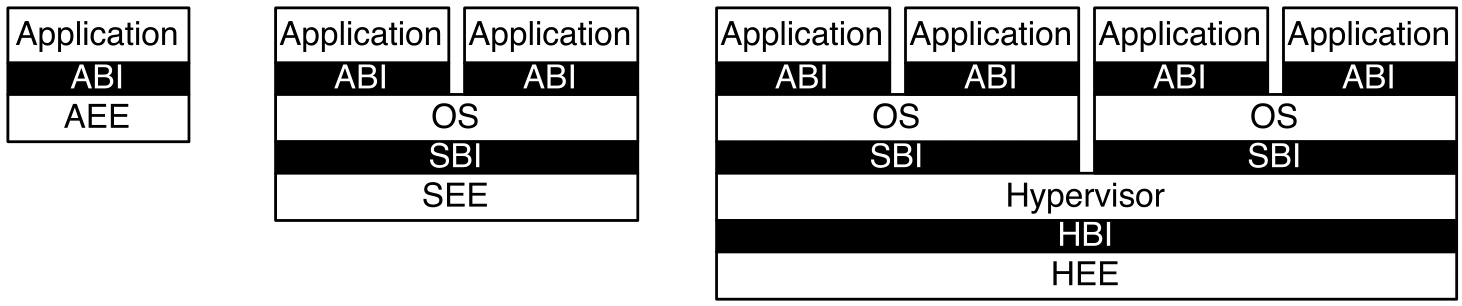
\includegraphics{figures/software-stacks.png}
%\caption{software-stacks}
%\end{figure}

上图中各个英文缩写对应的全称如下

\begin{itemize}
\item
  ABI: Application Binary Interface
\item
  AEE: Application Execution Environment
\item
  SBI: Supervisor Binary Interface
\item
  SEE: Supervisor Execution Environment
\item
  HBI: Hypervisor Binary Interface
\item
  HEE: Hypervisor Execution Environment
\end{itemize}

RISC-V通过各层之间的Binary
Interface实现了对下一层的抽象,方便了虚拟机的实现以及OS在不同RISC-V架构间的移植。采用了图中第二种结构,\href{https://github.com/riscv/riscv-pk}{bbl}在其中充当了SEE的角色。

\subsubsection{Privilege Levels}\label{privilege-levels}

RISC-V共有4种不同的特权级,与x86不同的是,RISC-V中特权级对应数字越小,权限越低

\begin{longtable}[c]{@{}cccc@{}}
\toprule
Level & Encoding & Name & Abbreviation\tabularnewline
\midrule
\endhead
0 & 00 & User/Application & U\tabularnewline
1 & 01 & Supervisor & S\tabularnewline
2 & 10 & Hypervisor & H\tabularnewline
3 & 11 & Machine & M\tabularnewline
\bottomrule
\end{longtable}

一个RISC-V的实现并不要求同时支持这四种特权级,可接受的特权级组合如下

\begin{longtable}[c]{@{}cll@{}}
\toprule
Number of levels & Supported Modes & Intended Usage\tabularnewline
\midrule
\endhead
1 & M & Simple embedded systems\tabularnewline
2 & M, U & Secure embedded systems\tabularnewline
3 & M, S, U & Systems running Unix-like operating systems\tabularnewline
4 & M, H, S, U & Systems running Type-1 hypervisors\tabularnewline
\bottomrule
\end{longtable}

目前官方的\href{https://github.com/riscv/riscv-isa-sim}{Spike}模拟器只部分实现了3个特权级。

\subsubsection{Control and Status
Registers}\label{control-and-status-registers}

RISC-V中各个特权级都有单独的Control and Status Registers
(CSRs),其中应当注意的有以下几个

\begin{longtable}[c]{@{}ll@{}}
\toprule
Name & Description\tabularnewline
\midrule
\endhead
sstatus & Supervisor status register\tabularnewline
sie & Supervisor interrupt-enable register\tabularnewline
stvec & Supervisor trap handler base address\tabularnewline
sscratch & Scratch register for supervisor trap handlers\tabularnewline
sepc & Supervisor exception program counter\tabularnewline
scause & Supervisor trap cause\tabularnewline
sbadaddr & Supervisor bad address\tabularnewline
sip & Supervisor interrupt pending\tabularnewline
sptbr & Page-table base register\tabularnewline
mstatus & Machine status register\tabularnewline
medeleg & Machine exception delegation register\tabularnewline
mideleg & Machine interrupt delegation register\tabularnewline
mie & Machine interrupt-enable register\tabularnewline
mtvec & Machine trap-handler base address\tabularnewline
mscratch & Scratch register for machine trap handlers\tabularnewline
mepc & Machine exception program counter\tabularnewline
mcause & Machine trap cause\tabularnewline
mbadaddr & Machine bad address\tabularnewline
mip & Machine interrupt pending\tabularnewline
\bottomrule
\end{longtable}

在继续阅读前,读者应当查阅\href{https://riscv.org/specifications/privileged-isa}{Privileged
Spec 1.9.1}以熟悉以上CSR的功能和用途。

\paragraph{CSR Instructions}\label{csr-instructions}

RISC-V
ISA中提供了一些修改CSR的原子操作,下面介绍之后常用到的\texttt{csrrw}指令

\begin{lstlisting}[language={C}]
# Atomic Read & Write Bit
cssrw rd, csr, rs
\end{lstlisting}

语义上等价的C++函数如下

\begin{lstlisting}[language={C}]
void cssrw(unsigned int& rd, unsigned int& csr, unsigned int& rs) {
   unsigned int tmp = rs;
   rd = csr;
   csr = tmp;
}
\end{lstlisting}

几种有趣的用法如下

\begin{lstlisting}[language={C}]
# csr = rs
cssrw x0, csr, rs

# csr = 0
cssrw x0, csr, x0

# rd = csr, csr = 0
cssrw rd, csr, x0

# swap rd and csr
cssrw rd, csr, rd
\end{lstlisting}


\section{“麻雀“OS--uCore}

为了学习OS,需要了解一个上百万代码的操作系统吗?自己写一个操作系统难吗?别被现在上百万行的Linux和Windows操作系统吓倒。当年Thompson乘他老婆带着小孩度假留他一人在家时,写了UNIX;当年Linus还是一个21岁大学生时完成了Linux雏形。站在这些巨人的肩膀上,我们能否也尝试一下做“巨人”的滋味呢?

MIT的Frans Kaashoek等在2006年参考PDP-11上的UNIX Version 6写了一个可在X86上跑的操作系统xv6(基于MIT License),用于学生学习操作系统。我们可以站在他们的肩膀上,基于xv6的设计,尝试着一步一步完成一个从“空空如也”到“五脏俱全”的“麻雀”操作系统—ucore,此“麻雀”包含虚存管理、进程管理、处理器调度、同步互斥、进程间通信、文件系统等主要内核功能,总的内核代码量(C+asm)不会超过5K行。充分体现了“小而全”的指导思想。

ucore的运行环境可以是真实的计算机系统,目前支持运行在X86,MIPS,ARM,RISC-V等计算机系统中。不过考虑到调试和开发的方便,我们可采用硬件模拟器,比如QEMU、BOCHS、VirtualBox、VMware Player等。ucore的开发环境主要是GCC中的gcc、gas、ld和MAKE等工具,也可采用集成了这些工具的IDE开发环境Eclipse-CDT。运行环境和开发环境既可以在Linux或Windows中使用。

那我们准备如何一步一步实现ucore呢?安装一个操作系统的开发过程,我们可以有如下的开发步骤:

\begin{enumerate}
	\def\labelenumi{\arabic{enumi}.}
	\item
	bootloader+toy
	ucore:理解操作系统启动前的硬件状态和要做的准备工作,了解运行操作系统的外设硬件支持,操作系统如何加载到内存中,理解两类中断--``外设中断'',``陷阱中断'',内核态和用户态的区别;
	\item
	物理内存管理:理解x86分段/分页模式,了解操作系统如何管理物理内存;
	\item
	虚拟内存管理:理解OS虚存的基本原理和目标,以及如何结合页表+中断处理(缺页故障处理)来实现虚存的目标,如何实现基于页的内存替换算法和替换过程;
	\item
	内核线程管理:理解内核线程创建、执行、切换和结束的动态管理过程,以及内核线程的运行周期等;
	\item
	用户进程管理:理解用户进程创建、执行、切换和结束的动态管理过程,以及在用户态通过系统调用得到内核中各种服务的过程;
	\item
	处理器调度:理解操作系统的调度过程和调度算法;
	\item
	同步互斥与进程间通信:理解同步互斥的具体实现以及对系统性能的影响,研究死锁产生的原因,如何避免死锁,以及线程/进程间如何进行信息交换和共享;
	\item
	文件系统:理解文件系统的具体实现,与进程管理和内存管理等的关系,缓存对操作系统IO访问的性能改进,虚拟文件系统(VFS)、buffer~cache和disk~driver之间的关系。
\end{enumerate}

其中每个开发步骤都是建立在上一个步骤之上的,就像搭积木,从一个一个小木块,最终搭出来一个小房子。在搭房子的过程中,完成从理解操作系统原理到实践操作系统设计与实现的探索过程。

%这个房子最终的建筑架构和建设进度如下图所示
%\textgreater{} (!可进一步标注处各个proj在下图中的位置)
%\begin{figure}[htbp]
%	\centering
%	\includegraphics{figures/ucore_arch.png}
%	\caption{ucore操作系统架构}
%\end{figure}

\section{小结}
本章以分析一个“hello world”程序的执行过程为例子,概要地介绍了操作系统运行的计算机硬件架构,包括CPU、内存和外设,并对操作系统的历史发展、定义、目标、接口、抽象和特征等进行了阐述。最后简要介绍了课程实验用到的ucore操作系统。
%\chapter{启动操作系统}\label{ch_boot}

\section{本章概要}

\paragraph{一句话描述}
站在操作系统的最底层,了解操作系统的启动,与物理硬件:CPU,内存和多种外设实现“零距离”接触,看到它们并管理它们!

\paragraph{概述}

其实这一章的内容与操作系统原理相关的部分较少,与计算机体系结构的细节相关的部分较多。但这些内容对写一个操作系统关系较大,要知道操作系统是直接与硬件打交道的软件,所以它需要``知道''需要硬件细节,才能更好地控制硬件。另一方面,部分内容涉及到操作系统的重要抽象--中断类异常,能够充分理解中断类异常为以后进一步了解进程切换、上下文切换等概念会很有帮助。

\paragraph{本章收获的知识}

\begin{itemize}
	\item
	与操作系统原理相关
	\item
	I/O设备管理:涉及程序循环检测方式和中断启动方式、I/O地址空间
	\item
	内存管理:基于分段机制的内存管理
	\item
	异常处理:涉及中断、故障和陷阱
	\item
	特权级:内核态和用户态
	\item
	计算机系统和编程
	\item
	硬件	
	\begin{itemize}
		\item
		计算机从加电到加载操作系统内核的整个过程
		\item
		OS内核在内存中的布局
		\item
		串口访问、时钟访问
	\end{itemize}
	\item
	软件	
	\begin{itemize}
		\item
		ELF执行文件格式
		\item
		栈的实现并实现函数调用栈跟踪函数
		\item
		调试操作系统
	\end{itemize}
\end{itemize}

\paragraph{本章涉及的实验}

本章的实验内容涉及的是写一个bootloader能够启动一个操作系统--ucore。在完成bootloader的过程中,逐渐增加bootloader和ucore的能力,涉及CPU的模式切换、解析ELF执行文件格式等,这对于理解操作系统的加载过程以及在操作系统在内存中的位置、内存管理、用户态与内核态的区别等有帮助。而相关project中bootloader和操作系统本身的字符显示的I/O处理、读硬盘数据的I/O处理、键盘/时钟的中断处理等内容,则是操作系统原理中一般在靠后位置提到的设备管理的实际体现。纵观操作系统的发展史,从早期到现在的操作系统主要功能之一就是完成繁琐的I/O处理,给上层应用提供比较简洁的I/O服务,屏蔽硬件处理的复杂性。这也是操作系统的虚拟机功能的体现。另外,本章还介绍了对硬件模拟器的使用,对操作系统的panic处理和远程debug功能的支持,这样有助于读者能够方便地分析操作系统中的错误和调试操作系统。由于本章涉及的硬件知识较多,无疑增大了读者的阅读难度,需要读者在结合阅读本章并实际动手实验来进行深入理解。

读者通过阅读本章的内容并动手实践相关的4个实验项目:

\begin{itemize}
	\item
	proj1:能够显示字符的bootloader
	\item
	proj2/3:可读ELF格式文件的bootloader和显示字符的ucore
	\item
	proj4:可管理中断和处理基于中断的键盘/时钟的ucore
\end{itemize}





\section{显示字符的toy
bootloader}\label{ux663eux793aux5b57ux7b26ux7684toy-bootloader}

\subsection{实验目标}\label{ux5b9eux9a8cux76eeux6807}

操作系统是一个软件,也需要通过某种手段加载并运行它。在这里我们将通过另外一个更加简单的软件-bootloader来完成这些工作。为此,我们需要完成一个能够切换到x86的保护模式并显示字符的bootloader,为将来启动操作系统做准备。proj1提供了一个非常小的bootloader,整个bootloader的大小小于512个字节,这样才能放到硬盘的主引导扇区中。
\textgreater{} 这里对x86的保护模式不必太在意,后续会进一步讲解

通过分析和实现这个bootloader,读者可以了解到: * 与操作系统原理相关 *
I/O设备管理:设备管理的基本概念,涉及简单的信息输出 *
内存管理:基于分段机制的存储管理,x86的实模式/保护模式以及切换到保护模式的方法
* 计算机系统和编程 * 硬件 * PC加电后启动bootloader的过程 *
通过串口/并口/CGA输出字符的方法 * 软件 * bootloader的文件组成 *
编译运行bootloader的过程 * 调试bootloader的方法 *
在汇编级了解栈的结构和处理过程

\subsection{proj1概述}\label{proj1ux6982ux8ff0}

\subsubsection{实现描述}\label{ux5b9eux73b0ux63cfux8ff0}

proj1实现了一个简单的bootloader,主要完成的功能是初始化寄存器内容,完成实模式到保护模式的转换,在保护模式下通过PIO方式控制串口、并口和CGA等进行字符串输出。

\subsubsection{项目组成}\label{ux9879ux76eeux7ec4ux6210}

{[}要点(非OSP):bootloader的编译生成过程{]}
lab1中包含的第一个工程小例子是proj1:一个可以切换到保护模式并显示字符串的bootloader。proj1的整体目录结构如下所示:

\begin{lstlisting}
    proj1 /
    |-- boot
    |   |-- asm.h
    |   |-- bootasm.S
    |   `-- bootmain.c
    |-- libs
    |   |-- types.h
    |   `-- x86.h
    |-- Makefile
    `-- tools
        |-- function.mk
        |-- gdbinit
        `-- sign.c

    3 directories, 9 files
\end{lstlisting}

其中一些比较重要的文件说明如下: * bootasm.S
:定义并实现了bootloader最先执行的函数start,此函数进行了一定的初始化,完成了从实模式到保护模式的转换,并调用bootmain.c中的bootmain函数。
*
bootmain.c:定义并实现了bootmain函数实现了通过屏幕、串口和并口显示字符串。
*
asm.h:是bootasm.S汇编文件所需要的头文件,主要是一些与X86保护模式的段访问方式相关的宏定义。
* types.h:包含一些无符号整型的缩写定义。 * x86.h:一些用GNU
C嵌入式汇编实现的C函数(由于使用了inline关键字,所以可以理解为宏)。 *
Makefile和function.mk:指导make完成整个软件项目的编译,清除等工作。 *
sign.c:一个C语言小程序,是辅助工具,用于生成一个符合规范的硬盘主引导扇区。
* gdbinit:用于gdb远程调试的初始命令脚本

从中,我们可以看出bootloader主要由bootasm.S和bootmain.c组成,当你完成编译后,你会发现这个bootloader只有区区的3百多字节。下面是编译运行bootloader的过程。

\begin{quote}
【提示】bootloader是一个超小的系统软件,在功能上与我们一般的应用软件不同,主要用于硬件简单初始化和加载运行操作系统。在编写bootloader的时候,需要了解它所处的硬件环境(比如它在内存中的起始地址,它的储存空间的位置和大小限制等)。而这些是编写应用软件不太需要了解的,因为操作系统和编译器帮助应用软件考虑了这些问题。
\end{quote}

\subsubsection{编译运行}\label{ux7f16ux8bd1ux8fd0ux884c}

\textbf{【实验 编译运行bootloader】}

在proj1下执行make,在proj1/bin目录下可生成一个ucore.img。ucore.img是一个包含了bootloader或OS的硬盘镜像,通过执行如下命令可在硬件虚拟环境
qemu中运行bootloader或OS:

\begin{lstlisting}
  make                     //生成bootloader和对应的主引导扇区
  make qemu          //通过qemu硬件模拟器来运行bootloader
  make clean          //清除生成的临时文件,bootloader和对应的主引导扇区
\end{lstlisting}

%\begin{figure}[htbp]
%\centering
%\includegraphics{figures/qemu_cha1.jpg}
%\caption{qemu\_img}
%\end{figure}

我们除了需要了解bootloader的功能外,还需要进一步了解bootloader的编译链接和最终执行码的生成过程,从而能够清楚生成的代码是否是我们所期望的。proj1中的Makefile是一个配置脚本,make软件工具能够通过Makefile完成管理bootloader的C/ASM代码生成执行码的整个过程。Makefile的内容比较复杂,不过读者在前期只需会执行make
{[}参数{]}来生成代码和清除代码即可。对于本实验的make的执行过程如下所示:

\begin{lstlisting}
    1. gcc -O2 -o tools/sign tools/sign.c
    2. i386-elf-gcc -fno-builtin -Wall -MD -ggdb -m32 -fno-stack-protector -O -nostdinc -Iinclude -Iinclude/x86 -c bootloader/bootmain.c -o obj/bootmain.o
    3. i386-elf-gcc -fno-builtin -Wall -MD -ggdb -m32 -fno-stack-protector -nostdinc -Iinclude -Iinclude/x86 -c bootloader/bootasm.S -o obj/bootasm.o
    4. i386-elf-ld  -N -e start -Ttext 0x7C00 -o obj/bootblock.o obj/bootasm.o obj/bootmain.o
    5. i386-elf-objdump -S obj/bootblock.o > obj/bootblock.asm
    6. i386-elf-objcopy -S -O binary obj/bootblock.o obj/bootblock.out
    7. sign.exe obj/bootblock.out obj/bootblock
       obj/bootblock.out size: 380 bytes
       build 512 bytes boot sector: obj/bootblock success!
    8. dd if=/dev/zero of=obj/ucore.img count=10000
       10000+0 records in
       10000+0 records out
       5120000 bytes (5.1 MB) copied, 0.509 s, 10.1 MB/s
    9. dd if=obj/bootblock of=obj/ucore.img conv=notrunc
       1+0 records in
       1+0 records out
       512 bytes (512 B) copied, 0.011 s, 46.5 kB/s
\end{lstlisting}

\textbf{这9步的含义是:}

\begin{lstlisting}
1. 编译生成sign执行程序,用于生成一个符合规范的硬盘主引导扇区;
2. 用gcc编译器编译bootmain.c,生成ELF格式的目标文件bootmain.o;
3. 用gas汇编器(gcc只是一个包装)编译bootasm.S,生成ELF格式的目标文件bootasm.o;
4. 用ld链接器把bootmain.o和bootasm.o链接在一起,形成生成ELF格式的执行文件bootblock.o;
5. 目标文件信息导出工具objdump反汇编bootblock.o,生成bootblock.asm,通过查看bootlock.asm内容,可以了解bootloader的实际执行代码;
6. 文件格式转换和拷贝工具objcopy把ELF格式的执行文件bootblock.o转换成binary格式的执行文件bootblock.out;
7. 通过sign执行程序,把bootblock.out(本身大小需要小于510字节)扩展到512字节,形成一个符合规范的硬盘主引导扇区bootblock;
8. 设备级转换与拷贝工具dd生成一个内容都为“0”的磁盘文件ucore.img;
9. 设备级转换与拷贝工具dd进一步把bootblock覆盖到ucore.img的前512个字节空间中,这样就可以把ucore.img作为一个可启动的硬盘被硬件模拟器qemu使用。
\end{lstlisting}

如果需要了解Makefile中的内容,需要进一步看看附录``ucore实验中的常用工具''一节。

\section{【背景】Intel
80386加电后启动过程}\label{ux80ccux666fintel-80386ux52a0ux7535ux540eux542fux52a8ux8fc7ux7a0b}

\textbf{【要点(非OSP):80836物理内存地址空间】}

\textbf{【要点(非OSP):80836加电后的第一条指令位】}

大家一般都知道bootloader负责启动操作系统,但bootloader自身是被谁加载并启动的呢?为了追根溯源,我们需要了解当计算机加电启动后,到底发生了什么事情。

对于绝大多数计算机系统而言,操作系统和应用软件是存放在磁盘(硬盘/软盘)、光盘、EPROM、ROM、Flash等可在掉电后继续保存数据的存储介质上。当计算机加电后,一般不直接执行操作系统,而是一开始会到一个特定的地址开始执行指令,这个特定的地址存放了系统初始化软件,通过执行系统初始化软件(可固化在ROM或Flash中,也称firmware,固件)完成基本I/O初始化和引导加载操作系统的功能。简单地说,系统初始化软件就是在操作系统内核运行之前运行的一段小软件。通过这段小软件的基本I/O初始化部分,我们可以初始化硬件设备、建立系统的内存空间映射图,从而将系统的软硬件环境带到一个合适的状态,以便为最终调用操作系统内核准备好正确的环境。最终系统初始化软件的引导加载部分把操作系统内核映像加载到RAM中,并将系统控制权传递给它。

对于基于Intel 80386的计算机而言,其中的系统初始化软件由BIOS (Basic Input
Output
System,即基本输入/输出系统,其本质是一个固化在主板Flash/CMOS上的软件)和位于软盘/硬盘引导扇区中的OS
Boot
Loader(在ucore中的bootasm.S和bootmain.c)一起组成。BIOS实际上是被固化在计算机ROM(只读存储器)芯片上的一个特殊的软件,为上层软件提供最底层的、最直接的硬件控制与支持。

以基于Intel
80386的计算机为例,计算机加电后,整个物理地址空间如下图所示:

%\begin{figure}[htbp]
%\centering
%\includegraphics{figures/3.13.1.png}
%\caption{3.13.1.png}
%\end{figure}

图2-1 基于Intel 80386的计算机物理地址空间

处理器处于实模式状态(在86386中,段机制一直存在,可进一步参考2.1.5
【背景】理解保护模式和分段机制),从物理地址0xFFFFFFF0开始执行。初始化状态的CS和EIP确定了处理器的初始执行地址,此时CS中可见部分-选择子(selector)的值为0xF000,而其不可见部分-基地址(base)的值为0xFFFF0000;EIP的值是0xFFF0,这样实际的线性地址(由于没有启动也机制,所以线性地址就是物理地址)为CS.base+EIP=0xFFFFFFF0。在0xFFFFFFF0这里只是存放了一条跳转指令,通过跳转指令跳到BIOS例行程序起始点。更详细的解释可以参考文献{[}1{]}的第九章的9.1节``INITIALIZATION
OVERVIEW''。另外,我们可以通过硬件模拟器qemu来进一步认识上述结果。

\subsubsection{实验2-1:通过qemu了解Intel
80386启动后的CS和EIP值,并分析第一条指令的内容}\label{ux5b9eux9a8c2-1ux901aux8fc7qemuux4e86ux89e3intel-80386ux542fux52a8ux540eux7684csux548ceipux503cux5e76ux5206ux6790ux7b2cux4e00ux6761ux6307ux4ee4ux7684ux5185ux5bb9}

\begin{enumerate}
\def\labelenumi{\arabic{enumi}.}
\item
  启动qemu并让其停到执行第一条指令前,这需要增加一个参数''-S'' qemu --S
\item
  这是qemu会弹出一个没有任何显示内容的图形窗口,显示如下:
\end{enumerate}

%\begin{figure}[htbp]
%\centering
%\includegraphics{figures/3.13.2.png}
%\caption{3.13.2.png}
%\end{figure}

\begin{enumerate}
\def\labelenumi{\arabic{enumi}.}
\setcounter{enumi}{2}
\item
  然后通过按''Ctrl+Alt+2''进入qemu的monitor界面,为了了解80386此时的寄存器内容,在monitor界面下输入命令
  ``info registers''
\end{enumerate}

%\begin{figure}[htbp]
%\centering
%\includegraphics{figures/3.13.3.png}
%\caption{3.13.3.png}
%\end{figure}

\begin{enumerate}
\def\labelenumi{\arabic{enumi}.}
\setcounter{enumi}{3}
\item
  可获得intel 80386启动后执行第一条指令前的寄存器内容,如下图所示
\end{enumerate}

%\begin{figure}[htbp]
%\centering
%\includegraphics{figures/3.13.4.png}
%\caption{3.13.4.png}
%\end{figure}

从上图中,我们可以看到EIP=0xfff0,CS的selector=0xf000,CS的base=0xfff0000。

BIOS做完计算机硬件自检和初始化后,会选择一个启动设备(例如软盘、硬盘、光盘等),并且读取该设备的第一扇区(即主引导扇区或启动扇区)到内存一个特定的地址0x7c00处,然后CPU控制权会转移到那个地址继续执行。至此BIOS的初始化工作做完了,进一步的工作交给了ucore的bootloader;ucore的bootloader会完成处理器从实模式到保护模式的转换,并从硬盘上读取并加载ucore。其大致流程如下图所示:

%\begin{figure}[htbp]
%\centering
%\includegraphics{figures/3.13.5.png}
%\caption{3.13.5.png}
%\end{figure}

图2-2 Intel80386启动过程

\section{【背景】设备管理:理解设备访问机制}\label{ux80ccux666fux8bbeux5907ux7ba1ux7406ux7406ux89e3ux8bbeux5907ux8bbfux95eeux673aux5236}

在本章涉及的bootloader和ucore都需要对I/O设备进行访问,比如通过串口、并口和CGA显示器显示字符串,读取硬盘数据,处理时钟中断等,已经需要读者用到操作系统的I/O设备管理知识了。为此,我们需要操作系统的设备管理进行一个简要描述。

在计算机系统中,操作系统需要管理各种设备,即给它们发送控制命令、捕获中断、错误处理等;为此专门设置了一个子系统:设备管理子系统来完成这些琐碎的工作。同时设备管理子系统还需要提供一个简单易用的统一接口,并尽可能地使其他内核功能组件或应用可通过这个统一接口访问所有的设备,即实现与设备的无关性。比如在proj1中,bootloader提供了一个显示字符的函数接口cons\_putc(位于bootmain.c中),在proj3中的提供了一个显示格式化信息的函数接口cprintf(位于printf.c中),这样操作系统的其他功能组件就可以直接使用这些简单易用的接口来输出信息,而不是通过繁琐的I/O命令与具体的设备打交道。cprintf的实现相对复杂,用到C语言的可变列表参数等,大家只要把它的功能理解为C语言应用库中的printf的简化版即可,并掌握最后是如何通过调用cons\_putc函数完成具体的I/O字符输出。

接下来,我们将从操作系统概念的角度对I/O设备组成、控制设备的方式进行阐述,并进一步对实验中所使用的基于Programmed
I/O (PIO)方式访问并口、CGA和硬盘进行具体分析。

\subsection{硬件设备简介}\label{ux786cux4ef6ux8bbeux5907ux7b80ux4ecb}

对于硬件设备而言,操作系统所关心的并不是硬件自身的设计,而是如何来对它进行控制,即该硬件所接受的控制命令、所完成的功能,以及所返回的出错。所以在设计操作系统的设备管理子系统时,需要了解计算机系统中I/O总线上连接的I/O控制器(比如PC机中的CGA控制器、串口控制器、并口控制器、时钟控制器8254,中断控制器8259等)。

I/O控制器在物理上包含三个层次:I/O地址空间、I/O接口和设备控制器。每个连接到I/O总线上的设备都有自己的I/O地址空间(即I/O端口),这也是CPU可以直接访问的地址。在
PC机中,支持基于I/O的I/O地址空间(通过IN/OUT这类的I/O访问指令访问),也支持基于内存的I/O地址空间(通过MOV等访存指令访问)。这些I/O访问请求通过I/O总线传递给I/O接口。

I/O接口是处于一组I/O端口和对应的设备控制器之间的一种硬件电路。它将I/O访问请求中的特定值转换成设备所需要的命令和数据;并且检测设备的状态变化,及时将各种状态信息写回到特定I/O地址空间,供操作系统通过I/O访问指令来访问。I/O接口包括键盘接口、图形接口、磁盘接口、总线鼠标、网络接口、括并口、串口、通用串行总线、PCMCIA接口和SCSI接口等。

设备控制器并不是所有I/O设备所必须的,只有少数复杂的设备才需要。它负责解释从I/O接口接收到的高级命令,并将其以适当的方式发送到I/O设备;并且对I/O设备发送的消息进行解释并修改I/O端口的状态寄存器。典型的设备控制器就是磁盘控制器,它将CPU发送过来的读写数据指令转换成底层的磁盘操作。

\subsection{控制设备的方式}\label{ux63a7ux5236ux8bbeux5907ux7684ux65b9ux5f0f}

操作系统对硬件设备的控制方式主要与三种:程序循环检测方式(Programmed
I/O,简称PIO)、中断驱动方式(Interrupt-driven I/O)、直接内存访问方式(DMA,
Direct Memory Access)。

在本章的proj1实验中,bootloader需要显示字符串,就是采用相对简单的PIO方式。PIO方式是一种通过CPU执行I/O端口指令来进行数据读写的数据交换模式,被广泛应用于硬盘、光驱等设备的基础传输模式中。这种I/O访问方式使用CPU
I/O端口指令来传送所有的命令、状态和数据,需要处理器全程参与,效率较低,但编程很简单。后面讲到的中断方式和直接内存访问(Direct
Memory Access,DMA)方式将更加高效。

对于程序循环检测方式而言,其控制方式体现在执行过程中通过不断地检测I/O设备的当前状态,来控制I/O操作。具体而言,在进行I/O操作之前,要循环地检测设备是否就绪;在I/O操作进行之中,要循环地检测设备是否已完成;在I/O操作完成之后,还要把输入的数据保存到内存(输入操作)。从硬件的角度来说,控制I/O的所有工作均由CPU来完成。所以此方式也称为繁忙等待方式(busy
waiting)或轮询方式(polling)。其缺点是在进行I/O操作时,一直占用CPU时间。

中断驱动方式的基本思路是用户任务通过系统调用函数来发起I/O操作。执行系统调用后会阻塞该任务,调度其他的任务使用CPU。在I/O操作完成时,设备向CPU发出中断,然后在中断服务例程中做进一步的处理。在中断驱动方式下,数据的每次读写还是通过CPU来完成。但是当I/O设备在进行数据处理时,CPU不必等待,可以继续执行其他的任务。采用这种方式可提供CPU利用率。编程方面,要考虑异步特性,相对麻烦一些。

使用DMA的控制方式,首先需要有DMA控制器。该控制器可集成在设备控制器中,也可集成在主板上。DMA控制器可以直接去访问系统总线,它能代替CPU指挥I/O设备与内存之间的数据传送,在执行完毕后再通知CPU。这种方式可大大减少CPU的执行开销,适合大数据量的设备数据传送。在编程方面,需要对DMA进行编程和异步中断编程,相对更加复杂一些。

\subsection{串口(serial
port)访问控制}\label{ux4e32ux53e3serial-portux8bbfux95eeux63a7ux5236}

串口是一个字符设备,proj1通过串口输出需要显示的信息。考虑到简单性,在proj1中没有对串口设备进行初始化,通过串口进行输出的过程也很简单:第一步:执行inb指令读取串口的I/O地址(COM1
+
COM\_LSR)的值,如果发现发现读出的值代表串口忙,则空转一小会(0x84是什么地址???);如果发现发现读出的值代表串口空闲,则执行outb指令把字符写到串口的I/O地址(COM1
+
COM\_TX),这样就完成了一个字符的串口输出。在proj1的bootmain.c中的serial\_putc函数完成了串口输出字符的工作,可参看其函数来了解大致实现。有关串口的硬件细节可参考附录
补充材料。

\subsection{并口(parallel
port)访问控制}\label{ux5e76ux53e3parallel-portux8bbfux95eeux63a7ux5236}

并口也是一个字符设备,proj1也通过并口输出需要显示的信息。考虑到简单性,在proj1中没有对并口设备进行初始化,通过并口进行输出的过程也很简单:第一步:执行inb指令读取并口的I/O地址(LPTPORT
+
1)的值,如果发现发现读出的值代表并口忙,则空转一小会再读;如果发现发现读出的值代表并口空闲,则执行outb指令把字符写到并口的I/O地址(LPTPORT
),这样就完成了一个字符的并口输出。在proj1的bootmain.c中的lpt\_putc函数完成了并口输出字符的工作,可参看其函数来了解大致实现。有关并口的硬件细节可参考附录
补充材料。

\subsection{CGA字符显示控制}\label{cgaux5b57ux7b26ux663eux793aux63a7ux5236}

彩色图形适配器(Color Graphics
Adapter,CGA)支持7种彩色和文本/图形显示方式,proj1也通过CGA进行信息显示。在80列×25行的文本字符显示方式下,有单色和16色两种显示方式。CGA显示控制器标配有16KB显示内存(占用内存地址范围0xb8000~0xbc000),可以看成是一种内存块设备,即bootloader和操作系统可以直接对显存进行内存访问,从而完成信息显示。在CGA显示控制器中,字符显示内存从线性地址0x000B8000开始,在80列×25行的范围内,共2000字符。每个字符需要两个字节来显示:第一个字节是想要显示的字符
,第二个字节用来确定前景色和背景色。前景色用低4位(0\textasciitilde{}3位)来表示,背景色用第4位到第6位来表示。最高位表示这个字符是否闪烁,1表示闪烁,0表示不闪烁。

如果要在屏幕上设置光标,则它须通过CGA显示控制器的I/O端口开控制。显示控制索引寄存器的I/O端口地址为0x3d4;数据寄存器I/O端口地址为0x3d5。CGA显示控制器内部有一系列寄存器可以用来访问其状态。0x3d4和0x3d5两个端口可以用来读写CGA显示控制器的内部寄存器。方法是先向0x3d4端口写入要访问的寄存器编号,再通过0x3d5端口来读写寄存器数据。存放光标位置的寄存器编号为14和15。两个寄存器合起来组成一个16位整数,这个整数就是光标的位置。比如0表示光标在第0行第0列,81表示第1
行第1列(设屏幕共有80列)。

在proj1中没有对CGA显示控制器进行初始化,通过CGA显示控制器进行输出的过程也很简单:首先通过in/out指令获取当前光标位置;然后根据得到的位置计算出显存的地址,直接通过访存指令写内存来完成字符的输出;最后通过in/out指令更新当前光标位置。在proj1的bootmain.c中的cga\_putc函数完成了CGA字符方式在某位置输出字符的工作,可参看其函数了解大致实现。

\subsection{设备管理封装}\label{ux8bbeux5907ux7ba1ux7406ux5c01ux88c5}

proj1把上述三种设备进行了一个封装,提供了一个cons\_puts函数接口:完成字符串的输出;和一个cons\_putc函数接口,完成字符的输出。其他内核功能模块只需调用cons\_puts或cons\_putc就可完成向上述三个设备进行字符输出的功能。这也就体现了设备管理子系统提供一个简单易用的统一接口的操作系统设计思想。

\section{【背景】内存管理:理解保护模式和分段机制}\label{ux80ccux666fux5185ux5b58ux7ba1ux7406ux7406ux89e3ux4fddux62a4ux6a21ux5f0fux548cux5206ux6bb5ux673aux5236}

为何要了解Intel 80386的保护模式和分段机制?首先,我们知道Intel
80386只有在进入保护模式后,才能充分发挥其强大的功能,提供更好的保护机制和更大的寻址空间,否则仅仅是一个快速的8086而已。没有一定的保护机制,任何一个应用软件都可以任意访问所有的计算机资源,这样也就无从谈起操作系统设计了。且Intel
80386的分段机制一直存在,无法屏蔽或避免。其次,在我们的bootloader设计中,涉及到了从实模式到保护模式的处理,我们的操作系统功能(比如分页机制)是建立在Intel
80386的保护模式上来设计的。如果我们不了解保护模式和分段机制,则我们面向Intel
80386体系结构的操作系统设计实际上是建立在一个空中楼阁之上。

\subsection{实模式}\label{ux5b9eux6a21ux5f0f}

80386的实模式是为了与8086处理器兼容而设置的。在实模式下,80386处理器就相当于一个快速的8086处理器。80386处理器被复位或加电的时候以实模式启动。这时候处理器中的各寄存器以实模式的初始化值工作。80386处理器在实模式下的存储器寻址方式和8086基本一致,由段寄存器的内容乘以16作为基地址,加上段内的偏移地址形成最终的物理地址,这时候它的32位地址线只使用了低20位,即可访问1MB的物理地址空间。在实模式下,80386处理器不能对内存进行分页机制的管理,所以指令寻址的地址就是内存中实际的物理地址。在实模式下,所有的段都是可以读、写和执行的。实模式下80386不支持优先级,所有的指令相当于工作在特权级(即优先级0),所以它可以执行所有特权指令,包括读写控制寄存器CR0等。这实际上使得在实模式下不太可能设计一个有保护能力的操作系统。实模式下不支持硬件上的多任务切换。实模式下的中断处理方式和8086处理器相同,也用中断向量表来定位中断服务程序地址。中断向量表的结构也和8086处理器一样,每4个字节组成一个中断向量,其中包括两个字节的段地址和两个字节的偏移地址。应用程序可以任意修改中断向量表的内容,使得计算机系统容易受到病毒、木马等的攻击,整个计算机系统的安全性无法得到保证。

\textbf{【历史:寻址空间:A20地址线与处理器向下兼容】}

Intel早期的8086
CPU提供了20根地址线,可寻址空间范围即0\textsubscript{2\^{}20(00000H}FFFFFH)的
1MB内存空间。但8086的数据处理位为16位,无法直接寻址1MB内存空间,所以8086提供了段地址加偏移地址的地址转换机制,就是我们常见的''段地址(16位):偏移地址(16位或有效地址)'',实际的计算方法为:''段地址*0x10H+偏移地址'',作为段地址的数据是放在段寄存器中的(16位),而作为位偏移地址的数据则是通过8086提供的寻址方式来计算而来的(16位)。而``段值:偏移''这种表示法能够表示的最大内存为0x10FFEEH(即0xFFFF0H~+~0xFFFFH),所以当寻址到超过1MB的内存时,会发生``回卷''(不会发生异常)。但下一代的基于Intel
80286 CPU的PC AT计算机系统提供了24根地址线,这样CPU的寻址范围变为
2\^{}24=16M,同时也提供了保护模式,可以访问到1MB以上的内存了,此时如果遇到``寻址超过1MB''的情况,系统不会再``回卷''了,这就造成了向下不兼容。为了保持完全的向下兼容性,IBM决定在PC
AT计算机系统上加个硬件逻辑,来模仿以上的回绕特征。他们的方法就是把A20地址线控制和键盘控制器的一个输出进行AND操作,这样来控制A20地址线的打开(使能)和关闭(屏蔽,禁止)。一开始时A20地址线控制是被屏蔽的(总为0),直到系统软件通过一定的I/O操作去打开它(参看bootloader的bootasm.S文件)。
当A20
地址线控制禁止时,则程序就像在8086中运行,1MB以上的地是不可访问的。在保护模式下A20地址线控制是要打开的。为了使能所有地址位的寻址能力,必须向键盘控制器8042发送一个命令。键盘控制器8042将会将它的的某个输出引脚的输出置高电平,作为
A20 地址线控制的输入。一旦设置成功之后,内存将不会再被绕回(memory
wrapping),这样我们就可以寻址intel 80286 CPU支持的16M
内存空间,或者是寻址intel 80386 以上级别CPU支持的所有 4G内存空间了。
8042键盘控制器的I/O端口是0x60~0x6f,实际上IBM
PC/AT使用的只有0x60和0x64两个端口(0x61、0x62和0x63用于与XT兼容目的)。8042通过这些端口给键盘控制器或键盘发送命令或读取状态。输出端口P2用于特定目的。位0(P20引脚)用于实现CPU复位操作,位1(P21引脚)用户控制A20信号线的开启与否。系统向输入缓冲(端口0x64)写入一个字节,即发送一个键盘控制器命令。可以带一个参数。参数是通过0x60端口发送的。
命令的返回值也从端口 0x60去读。
在proj1的bootasm.S中,``seta20.1''标号和``seta20.2''标号后的汇编代码即是用来完成A20地址线控制打开工作的。

\subsection{保护模式概述}\label{ux4fddux62a4ux6a21ux5f0fux6982ux8ff0}

简单地说,通过保护模式,可以把虚拟地址空间映射到不同的物理地址空间,且在超出预设的空间范围会报错(一种保护机制的体现),且可以保证处于低特权级的代码无法访问搞特权级的数据(另外一种保护机制的体现)。
只有在保护模式下,80386的全部32位地址才能有效,可寻址高达4G字节的线性地址空间和物理地址空间,可访问64TB(有2\textsuperscript{14个段,每个段最大空间为2}32字节)的虚拟地址空间,可采用分段存储管理机制和分页存储管理机制。这不仅为存储共享和保护提供了硬件支持,而且为实现虚拟存储提供了硬件支持。通过提供4个特权级和完善的特权检查机制,既能实现资源共享又能保证代码数据的安全及任务隔离。
在保护模式下,特权级总共有4个,编号从0(最高特权)到3(最低特权)。有3种主要的资源受到保护:内存,I/O地址空间以及执行特殊机器指令的能力。在任一时刻,intel
80386
CPU都是在一个特定的特权级下运行的,从而决定了代码可以做什么,不可以做什么。这些特权级经常被称为为保护环(protection
ring),最内的环(ring 0)对应于最高特权0,最外面的环(ring
3)一般给应用程序使用,对应最低特权3。在ucore中,CPU只用到其中的2个特权级:0(内核态)和3(用户态)。在保护模式下,我们可以通过查看CS寄存器的最低两位来了解当前正在运行的处理器是处于哪个特权级。

\subsection{分段机制的地址转换}\label{ux5206ux6bb5ux673aux5236ux7684ux5730ux5740ux8f6cux6362}

intel 80386
CPU提供了分段机制和分页机制两种内存管理方式,在当前计算机系统中是否需要这两种机制共存没有一个明确的答案,二者有它们各自独特的功能。在intel
80386
CPU中,只要进入保护模式,必然需要启动分段机制,且一直存在下去(分页不一定要一直存在),所以我们需要了解分段机制的原理。分段机制体现了内存中不同地址的一种转换/映射方式,即程序员编程所使用的地址(逻辑地址)和实际计算机中的物理地址需要通过分段机制来建立映射关系。分段机制将内存划分成以起始地址和长度限制这两个参数表示的内存块,这些内存块就称之为段(Segment)。编译器把源程序编译成执行程序时用到的代码段、数据段、堆和栈等概念在这里可以与段联系起来,二者在含义上是一致的。从操作系统原理上看,编译器实际上采用了基于分段的虚存管理方式来生成执行程序的,即应用程序员看到的逻辑地址和位于计算机上的物理地址之间有映射关系,二者可以是不同的。当然,后续章节中,我们还将介绍分页机制,即另一种使用更加广泛的地址转换/映射方式,这是操作系统实现虚存管理的重要基础。
简单地说,当CPU执行一条访存指令时(一个具体的指令),基于分段模式的具体硬件操作过程如下:

\begin{enumerate}
\def\labelenumi{\arabic{enumi}.}
\item
  根据指令的内容确定应该使用的段寄存器,比如取内存指令的内存地址所对应的数据段寄存器为DS;
\item
  根据段寄存器DS的值作为选择子,以此选择子值为索引,在段描述符表(可理解为一个大数组)找到索引指向的段描述符(可理解为数组中的元素);
\item
  在段描述符中取出基地址域(段的起始地址)和地址范围域(段的长度)的值;
\item
  将指令内容确定的地址偏移,与地址范围域的值比较,确保地址偏移小于地址范围,这样是为了确保地址范围不会跨出段的范围;(第一层保护)
\item
  根据指令的性质(当前指令的CS值的低两位)确定当前指令的特权级,需要高于当前指令访问的数据段的特权级;(第二层保护);
\item
  根据指令的性质(指令是做读还是写操作),需要当前指令访问的数据段可读或可写;(第三层保护)
\item
  将DS指向的段描述符中基地址域的值加上指令内容中指定的访存地址段内偏移值,形成实际的物理地址(实现地址转换),发到数据地址总线上,到物理内存中寻址,并取回该地址对应的数据内容。
  分段机制涉及4个关键内容:逻辑地址(Logical
  Address,应用程序员看到的地址,在操作系统原理上称为虚拟地址,以后提到虚拟地址就是指逻辑地址)、物理地址(Physical
  Address,
  实际的物理内存地址)、段描述符表(包含多个段描述符的``数组'')、段描述符(描述段的属性,及段描述符表这个``数组''中的``数组元素'')、段选择子(即段寄存器中的值,用于定位段描述符表中段描述符表项的索引)。
  虚拟地址到物理地址的转换主要分以下两步:
\item
  分段地址转换:CPU把虚拟地址(由段选择子selector和段偏移offset组成)中的段选择子值作为段描述符表的索引,找到表中对应的段描述符,然后把段描述符中保存的段基址加上段偏移值,形成线性地址(Linear
  Address,在操作系统原理上没有直接对应的描述,在没有启动分页机制的情况下,可认为就是物理地址;如果启动了分页机制,则可理解为第二级虚拟地址)。如果不启动分页存储管理机制,则线性地址等于物理地址。
\item
  分页地址转换,这一步中把线性地址转换为物理地址。(注意:这一步是可选的,由操作系统决定是否需要。在后续试验中会涉及。)
  上述转换过程对于应用程序员来说是不可见的。线性地址空间由一维的线性地址构成,在分段机制下的线性地址空间和物理地址空间对等。线性地址32位长,线性地址空间容量为4G字节。分段机制中虚拟地址到线性地址转换转换的基本过程如下图所示。
\end{enumerate}

%\begin{figure}[htbp]
%\centering
%\includegraphics{figures/3.15.1.png}
%\caption{3.15.1}
%\end{figure}

图1 分段机制中虚拟地址到线性地址转换转换基本过程

分段存储管理机制需要在启动保护模式的前提下建立。从上图可以看出,为了使得分段存储管理机制正常运行,需要在启动保护模式前建立好段描述符和段描述符表(参看bootasm.S中的``lgdt
gdtdesc''语句和gdt标号/gdtdesc标号下的数据结构)。

\subsubsection{段选择子}\label{ux6bb5ux9009ux62e9ux5b50}

\textbf{段选择子}是用来选择哪个描述符表和在该表中索引哪一个描述符的。选择子可以做为指针变量的一部分,从而对应用程序员是可见的,但是一般是由编译器(gcc)和链接工具(ld)来设置的。段选择子的内容一般放在段寄存器中。选择子的格式如下图所示:

%\begin{figure}[htbp]
%\centering
%\includegraphics{figures/3.15.2.png}
%\caption{3.15.2}
%\end{figure}

图2 段选择子结构

\textbf{索引(Index)}:在描述符表中从8192个描述符中选择一个描述符。处理器自动将这个索引值乘以8(描述符的长度),再加上描述符表的基址来索引描述符表,从而选出一个合适的描述符。

\textbf{表指示位(Table
Indicator,TI)}:选择应该访问哪一个描述符表。0代表应该访问全局描述符表(GDT);1代表应该访问局部描述符表(LDT)。LDT在实验中没有涉及。

\textbf{请求特权级(Requested Privilege
Level,RPL)}:用于段级的保护机制,比如,段选择子是CS,则这两位表示当前执行指令的处理器所处的特权级的值,从而你可以了解到当前处理器是处于用户态(Ring
3)还是内核态(Ring 0)。在后续试验中会进一步讲解。

\subsubsection{段描述符}\label{ux6bb5ux63cfux8ff0ux7b26}

在分段存储管理机制的保护模式下,每个段由如下三个参数进行定义:段基地址(Base
Address)、段界限(Limit)和段属性(Attributes)。

\textbf{段基地址}:即线性地址空间中段的起始地址。在80386保护模式下,段基地址长32位。因为基地址长度与寻址地址的长度相同,所以任何一个段都可以从32位线性地址空间中的任何一个字节开始,而不象实方式下规定的边界必须被16整除。
在实验中,一般都简化了段机制的使用,把所有段的段基地址设置为0。

\textbf{段界限}:规定段的大小。在80386保护模式下,段界限用20位表示,而且段界限可以是以单字节为最小单位或以4K字节为最小单位。在实验中,一般都简化了段机制的使用,把所有段的段界限设置为0xFFFFF,以4K字节为最小单位,即段的界限为4GB;

\textbf{类型(TYPE)}:用于区别不同类型的描述符。可表示所描述的段是代码段还是数据段,所描述的段是否可读/写/执行,段的扩展方向等。
\textbf{描述符特权级(Descriptor Privilege
Level)(DPL)}:用来实现保护机制。 \textbf{段存在位(Segment-Present
bit)}:如果这一位为0,则此描述符为非法的,不能被用来实现地址转换。如果一个非法描述符被加载进一个段寄存器,处理器会立即产生异常。图2显示了当存在位为0时,描述符的格式。操作系统可以任意的使用被标识为可用(AVAILABLE)的位。
\textbf{已访问位(Accessed
bit)}:当处理器访问该段(当一个指向该段描述符的选择子被加载进一个段寄存器)时,将自动设置访问位。操作系统可清除该位。
上述表示段的属性的参数通过段描述符(Segment
Descriptor)来表示,一个段描述符占8字节。段描述符的结构如下图所示:

%\includegraphics{figures/3.15.3.png} 

图2 段描述符结构

\subsubsection{全局描述符表}\label{ux5168ux5c40ux63cfux8ff0ux7b26ux8868}

全局描述符表的是一个保存多个段描述符的``数组'',其起始地址保存在全局描述符表寄存器GDTR中。GDTR长48位,其中高32位为基地址,低16位为段界限。由于GDT
不能用GDT本身之内的描述符进行描述定义,所以采用GDTR寄存器来表示GDT这一特殊的系统段。注意,全部描述符表中第一个段描述符设定为空段描述符。GDTR中的段界限以字节为单位。对于含有N个描述符的描述符表的段描述符实际所占空间通常可设为8\emph{N,若起始地址为gdt\_base,则结束地址为gdt\_base+8}N-1。可参考proj1中的bootasm.S中的gdt标号和gdtdesc标号下的内容,以及lgdt指令的操作数。
全局描述符表的第一项是不能被CPU使用,所以当一个段选择子的索引(Index)部分和表指示位(Table
Indicator)都为0的时(即段选择子指向全局描述符表的第一项时),可以当做一个空的选择子。当一个段寄存器被加载一个空选择子时,处理器并不会产生一个异常。但是,当用一个空选择子去访问内存时,则会产生异常。在proj1的实验中,值设置了三个段描述符,即NULL段、TEXT段和DATA段(都是4GB的访问范围)。

\subsection{分段机制的系统寄存器}\label{ux5206ux6bb5ux673aux5236ux7684ux7cfbux7edfux5bc4ux5b58ux5668}

80386
有4个寄存器来寻址描述发表等系统数据结构,用来实现段式内存管理。内存管理寄存器包括:

\begin{itemize}
\item
  全局描述符表寄存器 (Global Descriptor Table Register,GDTR
  ):指向全局段描述符表 GDT
\item
  局部描述符表寄存器 (Local Descriptor Table
  Register,LDTR):指向局部段描述符表 LDT~(目前用不上)
\item
  中断门描述符表寄存器 (Interrupt Descriptor Table
  Register,IDTR):指向一张包含中断处理子程序入口点的表(IDT)~
\item
  任务寄存器 (Task
  Register,TR):这个寄存器指向当前任务信息存放处,这些信息是处理器进行任务切换所需要的。(目前用不上)
  80386有四个32位的控制寄存器,分别命名位CR0、CR1、CR2和CR3。CR0包含指示处理器工作方式、启用和禁止分页管理机制、控制浮点协处理器操作的控制位。具体描述如下:
\item
  PE(保护模式允许 Protection Enable,比特位 0):设置PE
  将让处理器工作在保护模式下。复位PE将返回到实模式工作。
\item
  PG(分页允许 Paging, 比特位 31): PG
  指明处理器是否通过页表来转换线性地址到物理地址。在后续试验中将讲述如何设置PG位。
  CR0中的位5\textasciitilde{}位30是保留位,这些位的值必须为0。CR2及CR3由分页管理机制使用,将在后续试验中讲述。在80386中不能使用CR1,否则会引起无效指令操作异常。
\end{itemize}

\section{【实现】实模式到保护模式的切换}\label{ux5b9eux73b0ux5b9eux6a21ux5f0fux5230ux4fddux62a4ux6a21ux5f0fux7684ux5207ux6362}

BIOS把bootloader从硬盘(即是我们刚才生成的ucore.img)的第一个扇区(即是我们刚才生成的bootblock)读出来并拷贝到内存一个特定的地址0x7c00处,然后BIOS会跳转到那个地址((即CS=0,EIP=0x7c00))继续执行。至此BIOS的初始化工作做完了,进一步的工作交给了ucore的bootloader。

bootloader从哪里开始执行呢?我们【实验2-2
编译运行bootloader】中描述make工作过程的第五步就是生成了一个bootblock.asm,它的前面几行是:

\begin{lstlisting}
    obj/bootblock.o:     file format elf32-i386
    Disassembly of section .text:
    00007c00 <start>:
    .set CR0_PE_ON,      0x1         # protected mode enable flag
    .globl start
    start:
      .code16                     # Assemble for 16-bit mode
      cli                         # Disable interrupts
      7c00: fa                    cli
\end{lstlisting}

上述代码片段指出了bootblock(即bootloader)在0x7c00虚拟地址(在这里虚拟地址=线性地址=物理地址)处的指令为``cli'',如果读者再回头看看bootasm.S中的12\textasciitilde{}15行:

\begin{lstlisting}
    .globl start
    start:
      .code16                     # Assemble for 16-bit mode
      cli                         # Disable interrupts
      cld                         # String operations increment
\end{lstlisting}

就可以发现二者是完全一致的。而这个虚拟地址的设定是通过链接器ld完成的,我们【实验2-2
编译运行bootloader】中描述make工作过程的第四步: i386-elf-ld -N -e start
-Ttext 0x7C00 -o obj/bootblock.o obj/bootasm.o obj/bootmain.o

其中``-e start''指出了bootblock的入口地址为start,而``-Ttext
0x7C00''指出了代码段的起始地址为0x7c00,这也就导致start位置的虚拟地址为0x7c00。

从0x7c00开始,bootloader用了21条汇编指令完成了初始化和切换到保护模式的工作。其具体步骤如下:

\begin{enumerate}
\def\labelenumi{\arabic{enumi}.}
\item
  关中断,并清除方向标志,即将DF置``0'',这样(E)SI及(E)DI的修改为增量。
  cli \# Disable interrupts cld \# String operations increment
\item
  清零各数据段寄存器:DS、ES、FS xorw \%ax,\%ax \# Segment number zero
  movw \%ax,\%ds \# -\textgreater{} Data Segment movw \%ax,\%es \#
  -\textgreater{} Extra Segment movw \%ax,\%ss \# -\textgreater{} Stack
  Segment
\item
  使能A20地址线,这样80386就可以突破1MB访存现在,而可访问4GB的32位地址空间了。可回顾2.2.1节的【历史:A20地址线与处理器向下兼容】。
  seta20.1: inb \$0x64,\%al \# Wait for not busy testb \$0x2,\%al jnz
  seta20.1 movb \$0xd1,\%al \# 0xd1 -\textgreater{} port 0x64 outb
  \%al,\$0x64 seta20.2: inb \$0x64,\%al \# Wait for not busy testb
  \$0x2,\%al jnz seta20.2 movb \$0xdf,\%al \# 0xdf -\textgreater{} port
  0x60 outb \%al,\$0x60
\item
  建立全局描述符表(可回顾2.2.3节对全局描述符表的介绍),使能80386的保护模式(可回顾2.2.4节对CR0寄存器的介绍)。lgdt指令把gdt表的起始地址和界限(gdt的大小-1)装入GDTR寄存器中。而指令``movl
  \%eax,\%cr0''把保护模式开启位置为1,这时已经做好进入80386保护模式的准备,但还没有进入80386保护模式
  lgdt gdtdesc movl \%cr0, \%eax orl \$CR0\_PE\_ON, \%eax movl \%eax,
  \%cr0

  gdtdesc指出了全局描述符表(可以看成是段描述符组成的一个数组)的起始位置在gdt符号处,而gdt符号处放置了三个段描述符的信息
  gdt: SEG\_NULLASM \# null seg SEG\_ASM(STA\_X\textbar{}STA\_R, 0x0,
  0xffffffff) \# code seg SEG\_ASM(STA\_W, 0x0, 0xffffffff) \# data seg
  每个段描述符占8个字节,第一个是NULL段描述符,没有意义,表示全局描述符表的开始,紧接着是代码段描述符(位于全局描述符表的0x8处的位置),具有可读(STA\_R)和可执行(STA\_X)的属性,并且段起始地址为0,段大小为4GB;接下来是数据段描述符(位于全局描述符表的0x10处的位置),具有可读(STA\_R)和可写(STA\_W)的属性,并且段起始地址为0,段大小为4GB。
\item
  通过长跳转指令进入保护模式。80386在执行长跳转指令时,会重新加载\(PROT_MODE_CSEG的值(即0x8)到CS中,同时把\)protcseg的值赋给EIP,这样80386就会把CS的值作为全局描述符表的索引来找到对应的代码段描述符,设定当前的EIP为0x7c32(即protcseg标号所在的段内偏移),
  根据2.2.3节描述的分段机制中虚拟地址到线性地址转换转换的基本过程,可以知道线性地址(即物理地址)为:
  gdt{[}CS{]}.base\_addr+EIP=0x0+0x7c32=0x7c32 ljmp \$PROT\_MODE\_CSEG,
  \$protcseg
\item
  执行完上面的这条汇编语句后,bootloader让80386从实模式进入了保护模式。由于在访问数据或栈时需要用DS/ES/FS/GS和SS段寄存器作为全局描述符表的下标来找到相应的段描述符,所以还需要对DS/ES/FS/GS和SS段寄存器进行初始化,使它们都指向位于0x10处的段描述符(即gdt中的数据段描述符)。
  movw \$PROT\_MODE\_DSEG, \%ax \# Our data segment selector movw \%ax,
  \%ds \# -\textgreater{} DS: Data Segment movw \%ax, \%es \#
  -\textgreater{} ES: Extra Segment movw \%ax, \%fs \# -\textgreater{}
  FS movw \%ax, \%gs \# -\textgreater{} GS movw \%ax, \%ss \#
  -\textgreater{} SS: Stack Segment

  在保护模式下,所有的内存寻址将经过分段机制的存储管理来完成,即每个虚拟地址访问将经过分段机制转换成线性地址,由于这时还没有启动分页模式,所以线性地址就是物理地址。
\end{enumerate}

\section{【实现】设置栈}\label{ux5b9eux73b0ux8bbeux7f6eux6808}

只有设置好的合适大小和地址的栈内存空间(简称栈空间),才能有效地进行函数调用。这里为了减少汇编代码量,我们就通过C代码来完成显示。由于需要调用C语言的函数,所以需要自己建立好栈空间。设置栈的代码如下:

\begin{lstlisting}
movl    $start, %esp
\end{lstlisting}

由于start位置(0x7c00)前的地址空间没有用到,所以可以用来作为bootloader的栈,需要注意栈是向下长的,所以不会破坏start位置后面的代码。在后面的小节还会对栈进行更加深入的讲解。我们可以通过用gdb调试bootloader来进一步观察栈的变化:

\textbf{【实验】用gdb调试bootloader观察栈信息 }

\begin{enumerate}
\def\labelenumi{\arabic{enumi}.}
\item
  开两个窗口;在一个窗口中,在proj1目录下执行命令make;
\item
  在proj1目录下执行 ``qemu -hda bin/ucore.img -S
  -s'',这时会启动一个qemu窗口界面,处于暂停状态,等待gdb链接;
\item
  在另外一个窗口中,在proj1目录下执行命令 gdb obj/bootblock.o;
\item
  在gdb的提示符下执行如下命令,会有一定的输出:

\begin{lstlisting}
    (gdb) target remote :1234   #与qemu建立远程链接
    (gdb) break bootasm.S:68    #在bootasm.S的第68行“movl $start, %esp”设置一个断点
    (gdb) continue              #让qemu继续执行  
\end{lstlisting}

  这时qemu会继续执行,但执行到bootasm.S的第68行时会暂停,等待gdb的控制。这时可以在gdb中继续输入如下命令来分析栈的变化:

\begin{lstlisting}
    (gdb) info registers esp
    esp            0xffd6   0xffd6    #没有执行第68行代码前的esp值
    (gdb) si                          #执行第68行代码
    69        call bootmain
    (gdb) info registers esp
    esp            0x7c00   0x7c00   #当前的esp值,即栈顶
    (gdb) si
    bootmain () at boot/bootmain.c:87    #执行call汇编指令
    87      bootmain(void) {
    (gdb) info registers esp
    esp            0x7bfc   0x7bfc    #当前的esp值0x7bfc, 0x7bfc处存放了bootmain函数的返回地址0x7c4a,这可以通过下面两个命令了解  
    (gdb) x /4x 0x7bfc                  
    0x7bfc: 0x00007c4a      0xc031fcfa      0xc08ed88e      0x64e4d08e
    (gdb) x /4i 0x7c40
       0x7c40 <protcseg+14>:        mov    $0x7c00,%esp
       0x7c45 <protcseg+19>:        call   0x7c6c <bootmain>
       0x7c4a <spin>:       jmp    0x7c4a <spin>
       0x7c4c <gdt>:        add    %al,(%eax)
\end{lstlisting}
\end{enumerate}

\subsection{【提示】}\label{ux63d0ux793a}

在proj1中执行

\begin{lstlisting}
    make debug
\end{lstlisting}

则自动完成上述大部分前期工作,即qemu和gdb的加载,且gdb会自动建立于qemu的联接并设置好断点。具体实现可参看proj1的Makefile中于debug相关的内容和tools/gdbinit中的内容。

\section{【实现】显示字符串}\label{ux5b9eux73b0ux663eux793aux5b57ux7b26ux4e32}

bootloader只在CPU和内存中打转无法让读者很容易知道bootloader的工作是否正常,为此在成功完成了保护模式的转换后,就需要通过显示字符串来展示一下自己了。bootloader设置好栈后,就可以调用bootmain函数显示字符串了。在proj1中使用了显示器和并口两种外设来显示字符串,主要的代码集中在bootmain.c中。

这里采用的是很简单的基于Programmed I/O
(PIO)方式,PIO方式是一种通过CPU执行I/O端口指令来进行数据读写的数据交换模式,被广泛应用于硬盘、光驱等设备的基础传输模式中。这种I/O访问方式使用CPU
I/O端口指令来传送所有的命令、状态和数据,需要CPU全程参与,效率较低,但编程很简单。后面讲到的中断方式将更加高效。
在bootmain.c中的lpt\_putc函数完成了并口输出字符的工作。输出一个字符的流程(可参看bootmain.c中的lpc\_putc函数实现)大致如下:

\begin{enumerate}
\def\labelenumi{\arabic{enumi}.}
\item
  读I/O端口地址0x379,等待并口准备好;
\item
  向I/O端口地址0x378发出要输出的字符;
\item
  向I/O端口地址0x37A发出控制命令,让并口处理要输出的字符。
\end{enumerate}

在bootmain.c中的serial\_putc函数完成了串口输出字符的工作。输出一个字符的流程(可参看bootmain.c中的serial\_putc函数实现)大致如下:

\begin{enumerate}
\def\labelenumi{\arabic{enumi}.}
\item
  读I/O端口地址(0x3f8+5)获得LSR寄存器的值,等待串口输出准备好;
\item
  向I/O端口地址0x3f8发出要输出的字符;
\end{enumerate}

在bootmain.c中的cga\_putc函数完成了CGA字符方式在某位置输出字符的工作。输出一个字符的流程(可参看bootmain.c中的cga\_putc函数实现)大致如下:

\begin{enumerate}
\def\labelenumi{\arabic{enumi}.}
\item
  写I/O端口地址0x3d4,读I/O端口地址0x3d5,获得当前光标位置;
\item
  在光标的下一位置的显存地址空间上写字符,格式是黑色背景/白色字符;
\item
  设置当前光标位置为下一位置。
\end{enumerate}

proj1启动后的PC机内存布局如下图所示:

%\begin{figure}[htbp]
%\centering
%\includegraphics{figures/3.18.1.png}
%\caption{3.18.1}
%\end{figure}

自此,我们了解了一个小巧的bootloader的实现过程,但这还仅仅是百尺竿头的第一步,它还只能显示字符串,不能加载操作系统。我们还需要扩展bootloader的功能,让它能够加载操作系统。


\section{可读ELF格式文件的baby
bootloader}\label{ux53efux8bfbelfux683cux5f0fux6587ux4ef6ux7684baby-bootloader}

\subsection{实验目标}\label{ux5b9eux9a8cux76eeux6807}

接下来,我们需要完成一个能够读取位于硬盘中OS的代码内容并加载运行OS的bootloader,这需要bootloader能够读取硬盘扇区中的数据。由于OS采用ELF执行文件格式,所以bootloader能够解析ELF格式文件,把其中的代码和数据放到内存中正确的位置。Bootloader虽然增加了这么多功能,但整个bootloader的大小还是必须小于512个字节,这样才能放到只有512字节大小的硬盘主引导扇区中。
\textgreater{}
ucore内核不一定非要是ELF格式,基于binary格式的ucore内核也可以被bootloader识别与加载。

通过分析和实现这个bootloader,读者对设备管理的方式会有更加深入的理解,掌握bootloader/操作系统等底层系统软件是如何在保护模式下通过PIO(Programming
I/O,可编程I/O)方式访问块设备硬盘;理解如何在保护模式下解析并加载一个简单的ELF执行文件。

\subsection{proj2/3概述}\label{proj23ux6982ux8ff0}

\subsubsection{实现描述}\label{ux5b9eux73b0ux63cfux8ff0}

proj2基于proj1的主要实现一个可读硬盘并可分析ELF执行文件格式的bootloader,由于bootloader要放在512字节大小的主引导扇区中,所以不得不去掉部分显示输出的功能,确保整个bootloader的大小小于510个字节(最后两个字节用于硬盘主引导扇区标识,即``55AA'')。proj3在proj2的基础上增加了一个只能显示字符的第一代幼稚型操作系统ucore,用来验证proj2实现的bootloader能够正确从硬盘读出ucore并加载到正确的内存位置,并能把CPU控制权交给ucore。ucore在获得CPU控制权后,能够在保护模式下显示一个字符串,表明自己能够正常工作了

\subsubsection{项目组成}\label{ux9879ux76eeux7ec4ux6210}

这里我们分了两个project来完成此事。proj2是一个可分析ELF执行文件格式的例子,proj2整体目录结构如下所示:

\begin{lstlisting}
        proj2/
        |-- boot
        |   |-- asm.h
        |   |-- bootasm.S
        |   `-- bootmain.c
        |-- libs
        |   |-- elf.h
        |   |-- types.h
        |   `-- x86.h
        |-- Makefile
        ……
\end{lstlisting}

proj2与proj1类似,只是增加了libs/elf.h文件,并且bootmain.c中增加了对ELF执行文件的简单解析功能和读磁盘功能。

proj3建立在proj2基础之上,增加了一个只能显示字符的ucore操作系统,让bootloader能够把这个操作系统从硬盘上读到内存中,并跳转到ucore的起始处执行ucore的功能。proj3整体目录结构如下所示:

\begin{lstlisting}
        proj3
        |-- boot
        |   |-- asm.h
        |   |-- bootasm.S
        |   `-- bootmain.c
        |-- kern
        |   |-- driver
        |   |   |-- console.c
        |   |   `-- console.h
        |   |-- init
        |   |   `-- init.c
        |   `-- libs
        |       `-- stdio.c
        |-- libs
        |   |-- elf.h
        |   |-- error.h
        |   |-- printfmt.c
        |   |-- stdarg.h
        |   |-- stdio.h
        |   |-- string.c
        |   |-- string.h
        |   |-- types.h
        |   `-- x86.h
        |-- Makefile
        ……
\end{lstlisting}

proj3相对于proj2增加了ucore相关的文件,下面简要说明一下: *
libs目录下的printfmt.c:完成类似C语言的printf中的格式化处理; *
libs目录下的string.c:完成类似C语言的str***相关的字符串处理函数; *
libs目录下的st\emph{.h:是支持上述两个库函数(可被内核和用户应用共享)的.h文件;
} kern/init目录下的init.c:完成ucore的初始化工作; *
kern/driver目录下的console.c:提供并口/串口/CGA方式的字符输出的console驱动;
* kern/libs/stdio.c:提供内核方式下的的cprintf函数功能;

\subsubsection{编译运行}\label{ux7f16ux8bd1ux8fd0ux884c}

那接下来是如何生成一个包含了bootloader和ucore操作系统的硬盘镜像呢?我们先修改proj3目录下的Makefile,在其第五行

\begin{lstlisting}
        V       := @
\end{lstlisting}

的最前面增加一个``\#''(目的是让make工具程序详细显示整个project的编译过程),这样就把这行给注释了。然后在proj3目录下执行make,可以看到:

\begin{lstlisting}
        ……
        ld -m    elf_i386 -Ttext 0x100000 -e kern_init -o bin/kernel obj/kern/init/init.o obj/kern/libs/printf.o obj/kern/driver/console.o obj/libs/printfmt.o obj/libs/string.o
        ……
        dd if=bin/kernel of=bin/ucore.img seek=1 conv=notrunc
\end{lstlisting}

这两步是生成ucore的关键。第一步把ucore涉及的各个.o目标文件链接起来,并在bin目录下形成ELF文件格式的文件kernel,这就是我们第一个ucore操作系统,而且设定ucore的执行入口地址在0x10000,即kern\_init函数的起始位置。这也就意味着bootloader需要把读出的kernel文件的代码段+数据段放置在0x10000起始的内存空间。第二步是把bin目录下的kernel文件直接覆盖到ucore.img(虚拟硬盘的文件)的bootloader所处扇区(即第一个扇区,主引导扇区)之后的扇区(第二个扇区)。如果一个扇区大小为512字节,这kernel覆盖的扇区数为上取整(kernel的大小/512字节)。

编译后运行proj3的示意图如下所示:

%\begin{lstlisting}
%![qemu_cha1](figures/qemu_cha2.jpg)
%\end{lstlisting}


\section{【背景】访问硬盘数据控制}\label{ux80ccux666fux8bbfux95eeux786cux76d8ux6570ux636eux63a7ux5236}

bootloader让80386处理器进入保护模式后,下一步的工作就是从硬盘上加载并运行OS。考虑到实现的简单性,bootloader的访问硬盘都是LBA模式的PIO(Program
IO)方式,即所有的I/O操作是通过CPU访问硬盘的I/O地址寄存器完成。

一般主板有2个IDE通道(是硬盘的I/O控制器),每个通道可以接2个IDE硬盘。第一个IDE通道通过访问I/O地址0x1f0-0x1f7来实现,第二个IDE通道通过访问0x170-0x17f实现。每个通道的主从盘的选择通过第6个I/O偏移地址寄存器来设置。具体参数见下表。

\begin{lstlisting}
I/O地址   功能
0x1f0   读数据,当0x1f7不为忙状态时,可以读。
0x1f2   要读写的扇区数,每次读写前,需要指出要读写几个扇区。
0x1f3   如果是LBA模式,就是LBA参数的0-7位
0x1f4   如果是LBA模式,就是LBA参数的8-15位
0x1f5   如果是LBA模式,就是LBA参数的16-23位
0x1f6   第0~3位:如果是LBA模式就是24-27位   第4位:为0主盘;为1从盘
第6位:为1=LBA模式;0 = CHS模式     第7位和第5位必须为1
0x1f7   状态和命令寄存器。操作时先给命令,再读取内容;如果不是忙状态就从0x1f0端口读数据
\end{lstlisting}

硬盘数据是储存到硬盘扇区中,一个扇区大小为512字节。读一个扇区的流程大致为通过outb指令访问I/O地址:0x1f2\textasciitilde{}-0x1f7来发出读扇区命令,通过in指令了解硬盘是否空闲且就绪,如果空闲且就绪,则通过inb指令读取硬盘扇区数据都内存中。可进一步参看bootmain.c中的readsect函数实现来了解通过PIO方式访问硬盘扇区的过程。

\section{【背景】理解ELF文件格式}\label{ux80ccux666fux7406ux89e3elfux6587ux4ef6ux683cux5f0f}

由于本章的project中,bootloader会访问ELF(Executable and linking
format)格式的ucore,并把ucore加载到内存中。所以,在这里我们需要简单介绍一下ELF文件格式,以帮助我们理解ucore的整个编译、链接和加载的过程,特别是希望读者对ld链接器用到的链接地址(Link
address)和操作系统相关的加载地址(Load address)有更清楚的了解。

ELF文件格式是Linux系统下的一种常用目标文件(object
file)格式,有三种主要类型。可重定位文件(relocatable
file)类型和共享目标文件(shared object
file)类型在本实验中没有涉及。本实验的OS文件类型是可执行文件(executable
file)类型,这种ELF文件格式类型提供程序的进程映像,加载程序的内存地址描述等。

简单地说,bootloader通过解析ELF格式的ucore,可以了解到ucore的代码段(机器码)/数据段(初始化的变量)等在文件中的位置和大小,以及应该放到内存中的位置;可了解ucore的BSS段(未初始化的变量,具体内容没有保存在文件中)的内存位置和大小。这样bootloader就可以把ucore正确地放置到内存中,便于ucore的正确执行。

这里只分析与本章相关的ELF可执行文件类型。ELF的执行文件映像如下所示:

\begin{figure}[htbp]
\centering
\includegraphics{figures/3.2.4.1.png}
\caption{3.2.4.1}
\end{figure}

ELF的文件头包含整个执行文件的数据结构elf
header,描述了整个执行文件的组织结构。其定义在proj2/3中的elf.h文件中:

\begin{lstlisting}
struct elfhdr {
    uint32_t e_magic;     // must equal ELF_MAGIC
    uint8_t e_elf[12];
    uint16_t e_type;      // 1=relocatable, 2=executable, 3=shared object, 4=core image
    uint16_t e_machine;   // 3=x86, 4=68K, etc.
    uint32_t e_version;   // file version, always 1
    uint32_t e_entry;     // entry point if executable
    uint32_t e_phoff;     // file position of program header or 0
    uint32_t e_shoff;     // file position of section header or 0
    uint32_t e_flags;     // architecture-specific flags, usually 0
    uint16_t e_ehsize;    // size of this elf header
    uint16_t e_phentsize; // size of an entry in program header
    uint16_t e_phnum;     // number of entries in program header or 0
    uint16_t e_shentsize; // size of an entry in section header
    uint16_t e_shnum;     // number of entries in section header or 0
    uint16_t e_shstrndx;  // section number that contains section name strings
};
\end{lstlisting}

program
header描述与程序执行直接相关的目标文件结构信息,用来在文件中定位各个段的映像,同时包含其他一些用来为程序创建进程映像所必需的信息。可执行文件的程序前面部分有一个program
header结构的数组,
每个结构描述了一个``段''(segment)或者准备程序执行所必需的其它信息。目标文件的
``段''(segment) 包含一个或者多个 ``节区''(section)
,也就是``段内容(Segment Contents)'' 。program
header仅对于可执行文件和共享目标文件有意义。可执行目标文件在elfhdr的e\_phentsize和e\_phnum成员中给出其自身程序头部的大小。程序头部的数据结构如下表所示:

\begin{lstlisting}
struct proghdr {
    uint32_t p_type;   // loadable code or data, dynamic linking info,etc.
    uint32_t p_offset; // file offset of segment
    uint32_t p_va;     // virtual address to map segment
    uint32_t p_pa;     // physical address, not used
    uint32_t p_filesz; // size of segment in file
    uint32_t p_memsz;  // size of segment in memory (bigger if contains bss)
    uint32_t p_flags;  // read/write/execute bits
    uint32_t p_align;  // required alignment, invariably hardware page size
};
\end{lstlisting}

\textbf{链接地址(Link address)和加载地址(Load address)}

Link~Address是指编译器指定代码和数据所需要放置的内存地址,由链接器配置。Load~Address是指程序被实际加载到内存的位置。一般由可执行文件结构信息和加载器可保证这两个地址相同。Link
Addr和LoadAddr不同会导致:

\begin{lstlisting}
直接跳转位置错误
直接内存访问(只读数据区或bss等直接地址访问)错误
堆和栈等的使用不受影响,但是可能会覆盖程序、数据区域
\end{lstlisting}

也存在Link地址和Load地址不一样的情况(如动态链接库)。在proj3中,bootloader和ucore的链接地址和加载地址是一致的。

\begin{figure}[htbp]
\centering
\includegraphics{figures/3.2.4.2.png}
\caption{3.2.4.2}
\end{figure}

\section{【背景】操作系统执行代码的组成}\label{ux80ccux666fux64cdux4f5cux7cfbux7edfux6267ux884cux4ee3ux7801ux7684ux7ec4ux6210}

ucore通过gcc编译和ld链接,形成了ELF格式执行文件kernel(位于bin目录下),这样kernel的内部组成与一般的应用程序差别不大。一般而言,一个执行程序的内容是至少由
bss段、data段、text段三大部分组成。 * BSS段:BSS(Block Started by
Symbol)段通常是指用来存放执行程序中未初始化的全局变量的一块存储区域。BSS段属于静态内存分配的存储空间。
* 数据段:数据段(Data
Segment)通常是指用来存放执行程序中已初始化的全局变量的一块存储区域。数据段属于静态内存分配的存储空间。
* 代码段:代码段(Code Segment/Text
Segment)通常是指用来存放程序执行代码的一块存储区域。这部分区域的大小在程序运行前就已经确定,并且内存区域通常属于只读,
某些CPU架构也允许代码段为可写,即允许修改程序。在代码段中,也有可能包含一些只读的常数变量,例如字符串常量等。

ucore和一般应用程序一样,首先是保存在像硬盘这样的非易失性存储介质上,当需要运行时,被加载到内存中。这时,需要把代码段、数据段的内容拷贝到内存中。对于位于BSS段中的未初始化的全局变量,执行程序一般认为其值为零。所以需要把BSS段对应的内存空间清零,确保执行代码的正确运行。可查看init文件中的kern\_init函数的第一个执行语句``memset(edata,
0, end - edata);''。

随着ucore的执行,可能需要进行函数调用,这就需要用到栈(stack);如果需要动态申请内存,这就需要用到堆(heap)。堆和栈是在操作系统执行过程中动态产生和变化的,并不存在于表示内核的执行文件中。栈又称堆栈,
是用户存放程序临时创建的局部变量,即函数中定义的变量(但不包括static声明的变量,static意味着在数据段中存放变量)。除此以外,在函数被调用时,其参数也会被压入发起调用函数的栈中,并且待到调用结束后,函数的返回值也会被存放回栈中。由于栈的先进后出特点,所以栈特别方便用来保存/恢复调用现场。可以把栈看成一个寄存、交换临时数据的内存区。堆是用于存放运行中被动态分配的内存空间,它的大小并不固定,可动态扩张或缩减,这需要操作系统自己进行有效的管理。

\section{【实现】bootloader加载并运行ucore}\label{ux5b9eux73b0bootloaderux52a0ux8f7dux5e76ux8fd0ux884cucore}

了解完proj2/3的组成与编译,并大致理解上述两个背景知识后,我们就可以分析bootloader加载并运行ucore操作系统的工作流程。

硬盘数据是储存到硬盘扇区中,一个扇区大小为512字节。读一个扇区的流程可参看bootmain.c中的readsect函数实现。大致如下:

\begin{enumerate}
\def\labelenumi{\arabic{enumi}.}
\item
  读I/O地址0x1f7,等待磁盘准备好;
\item
  写I/O地址0x1f2\textasciitilde{}0x1f5,0x1f7,发出读取第offseet个扇区处的磁盘数据的命令;
\item
  读I/O地址0x1f7,等待磁盘准备好;
\item
  连续读I/O地址0x1f0,把磁盘扇区数据读到指定内存。
\end{enumerate}

这个函数是被bootloader用于读取硬盘上的ucore操作系统。bootloader为了读取硬盘上的ucore操作系统,将调用bootmain函数首先读取了位于主引导扇区的后的连续8个扇区(可参见bootmain函数中的第一条语句),并把数据放到0x10000处(可回顾一下2.7.1中描述链接bin/kernel的过程),并按照数据结构elfhdr来解析这块4KB大小的数据;如果其e\_magic数据域不等于ELF\_MAGIC(即0x464C457F),则表示这个不是标准的ELF格式的文件;如果等于ELF\_MAGIC,则继续解析,并根据其e\_phnum数据域的值来读取多个program
header,并根据program
header的信息,了解到ucore中各个segment的起始位置和大小,然后把放在硬盘上的相关segment读入到内存中。

\textbf{【实验】分析kernel并在bootloader中显示kernel的segment信息}

\begin{enumerate}
\def\labelenumi{\arabic{enumi}.}
\item
  在proj3目录下执行命令make,则会在bin目录下生成kernel,即ELF执行格式文件的操作系统ucore;
\item
  在proj3目录下执行命令 readelf -h bin/kernel,可得到有关elf
  header的如下信息

\begin{lstlisting}
ELF Header:
  Magic:   7f 45 4c 46 01 01 01 00 00 00 00 00 00 00 00 00 
  Class:                             ELF32
  Data:                              2's complement, little endian
  Version:                           1 (current)
  OS/ABI:                            UNIX - System V
  ABI Version:                       0
  Type:                              EXEC (Executable file)
  Machine:                           Intel 80386
  Version:                           0x1
  Entry point address:               0x100000
  Start of program headers:          52 (bytes into file)
  Start of section headers:          19872 (bytes into file)
  Flags:                             0x0
  Size of this header:               52 (bytes)
  Size of program headers:           32 (bytes)
  Number of program headers:         3
  Size of section headers:           40 (bytes)
  Number of section headers:         17
  Section header string table index: 14
\end{lstlisting}

  从中,我们可以看到kernel的入口点在0x100000,program
  header相对文件的偏移位置在52,elf header的大小为52字节,program
  header的大小为32字节。
\item
  在proj3目录下执行命令 readelf -l bin/kernel,可得到有关program
  header的如下信息 Elf file type is EXEC (Executable file) Entry point
  0x100000 There are 3 program headers, starting at offset 52

\begin{lstlisting}
Program Headers:
  Type           Offset   VirtAddr   PhysAddr   FileSiz MemSiz  Flg Align
  LOAD           0x001000 0x00100000 0x00100000 0x01038 0x01038 R E 0x1000
  LOAD           0x002038 0x00102038 0x00102038 0x00004 0x00004 RW  0x1000
  GNU_STACK      0x000000 0x00000000 0x00000000 0x00000 0x00000 RW  0x4

 Section to Segment mapping:
  Segment Sections...
   00     .text .rodata 
   01     .data 
   02     
\end{lstlisting}
\end{enumerate}

从中,我们可以看到kernel的入口点在0x100000,代码段位于0x100000,大小为0x1038;数据段位于0x102038,大小为0x04。

\textbf{【实验】用gdb调试bootloader,并在gdb中显示kernel的segment信息}

我们还可通过用gdb调试bootloader进行验证,具体步骤如下: 5.
开两个窗口;在一个窗口中,在proj3目录下执行命令make; 6.
在proj3目录下执行 ``qemu -hda bin/ucore.img -S
--s'',这时会启动一个qemu窗口界面,处于暂停状态,等待gdb链接; 7.
在另外一个窗口中,在proj3目录下执行命令 gdb obj/bootblock.o; 8.
在gdb的提示符下执行如下命令,会有一定的输出: (gdb) target remote :1234
\#与qemu建立远程链接 (gdb) break bootmain.c:100
\#在bootmain.c的第100行设置一个断点 (gdb) continue \#让qemu继续执行\\
这时qemu会继续执行,但执行到bootmain.c的第100行时会暂停,等待gdb的控制。这时可以在gdb中继续输入如下命令来参考kernel的信息:
(gdb) p /x \emph{(struct elfhdr })0x10000 \#按struct
elfhdr结构显示0x10000处内容 \$7 = \{e\_magic = 0x464c457f, e\_elf =
\{0x1, 0x1, 0x1, 0x0, 0x0, 0x0, 0x0, 0x0, 0x0, 0x0, 0x0, 0x0\}, e\_type
= 0x2, e\_machine = 0x3, e\_version = 0x1, e\_entry = 0x100000, e\_phoff
= 0x34, e\_shoff = 0x4550, e\_flags = 0x0, e\_ehsize = 0x34,
e\_phentsize = 0x20, e\_phnum = 0x3, e\_shentsize = 0x28, e\_shnum =
0x11, e\_shstrndx = 0xe\}
查看bootmain函数,可以知道,此时在0x10000处已经读入了kernel的ELF头信息,有三个program
header 表(e\_phnum值),继续在gdb中敲入命令,可以得到更多信息: (gdb) next
\#执行下一条指令 (gdb) p /x \emph{ph \#获得text段的program header表信息
\$5 = \{p\_type = 0x1, p\_offset = 0x1000, p\_va = 0x100000, p\_pa =
0x100000, p\_filesz = 0x1038, p\_memsz = 0x1038, p\_flags = 0x5,
p\_align = 0x1000\} (gdb) next \#执行下一条指令 (gdb) next
\#执行下一条指令 (gdb) p /x }ph \#获得data段的program header表信息 \$6 =
\{p\_type = 0x1, p\_offset = 0x2038, p\_va = 0x102038, p\_pa = 0x102038,
p\_filesz = 0x4, p\_memsz = 0x4, p\_flags = 0x6, p\_align = 0x1000\}

\begin{lstlisting}
对照readelf命令输出的信息,可以发现bootloader正确读出了text段和data段的program header表信息,并根据这些信息调用如下函数
    -->readseg(ph->p_va, ph->p_memsz, ph->p_offset);
        -->readsect((uint8_t *)va, offset);
\end{lstlisting}

把这两个段的内容读入到正确的线性内存地址中。然后再根据e\_entry =
0x100000,跳转到0x100000处去执行,这其实就是把处理器控制权转移给了ucore了。

\section{【实现】可输出字符串的ucore}\label{ux5b9eux73b0ux53efux8f93ux51faux5b57ux7b26ux4e32ux7684ucore}

proj3包含了一个只能输出字符串的简单ucore操作系统,虽然简单,但它也体现了操作系统的一些结构和特征,比如它具有:

\begin{itemize}
\item
  完成给ucore的BSS段清零并显示一个字符串的内核初始化子系统(init.c)
\item
  提供串口/并口/CGA显示的驱动程序子系统(console.c)
\item
  提供公共服务的操作系统函数库子系统(printf.c printfmt.c string.c)
\end{itemize}

这体现了操作系统的一个基本特征:资源管理器。从操作系统原理我们可以知道一台计算机就是一组资源,这些资源用于对数据的移动、存储和处理并进行控制。在proj3中的ucore操作系统目前只提供了对串口/并口/CGA这三种I/O设备的硬件资源的访问,每个I/O设备的操作都有自己特有的指令集或控制信号(对照一下serial\_putc/lpt\_putc/cga\_putc函数的实现),操作系统隐藏这些细节,并提供了统一的接口(看看cprintf函数的实现),因此程序员可以使用简单的printf函数来写这些设备,达到显示数据的效果。目前操作系统的逻辑结构图架构如下图所示:

\begin{figure}[htbp]
\centering
\includegraphics{figures/3.2.7.1.png}
\caption{3.2.7.1}
\end{figure}

在PC中的地址空间布局图如下所示:

\begin{figure}[htbp]
\centering
\includegraphics{figures/3.2.7.2.png}
\caption{3.2.7.2}
\end{figure}


\section{可管理中断并处理中断方式I/O的ucore}\label{ux53efux7ba1ux7406ux4e2dux65adux5e76ux5904ux7406ux4e2dux65adux65b9ux5f0fioux7684ucore}

\subsection{实验目标}\label{ux5b9eux9a8cux76eeux6807}

前面的project都没有引入中断机制,所以bootloader和ucore都是正常地顺序执行,不会受到外界(比如外设)的``干扰''。虽然实现简单,但无法解决上述问题。我们需要扩展ucore的功能,让ucore能够支持中断,这需要读者了解基本的80386硬件中断机制,对保护模式有更深入的了解;需要清楚在中断的处理过程中,硬件主动完成了什么事情,软件在硬件完成的基础上又要完成哪些事情。通过学习和实践,读者可以了解清楚上述问题,并进一步知道通过操作系统的中断处理例程(Interrupt
Process Routine, IPR)完成设备请求处理的方法等。

\subsection{proj4概述}\label{proj4ux6982ux8ff0}

\subsubsection{实现描述}\label{ux5b9eux73b0ux63cfux8ff0}

proj4建立在proj3.1的基础上,实现了一个通过中断机制完成设备(键盘、串口和时钟)中断请求处理的ucore。简单地说proj4扩展与中断相关的工作有两个,一个是初始化中断,涉及初始化中断控制器8259A(打通外设与CPU的通路)和中断门描述符表(建立外设中断与中断服务例程的联系)和各种外设。以proj4的ucore为例,操作系统内核启动以后,kern\_init函数(kern/init/init.c)通过调用pic\_init函数完成对中断控制器的初始化工作,调用idt\_init函数完成了对整个中断门描述符表的创建,调用cons\_init和clock\_init函数完成对串口、键盘和时钟外设的中断初始化工作。

ucore的另一个重要工作是中断服务,即收到中断后,对中断进行处理的中断服务例程(比如收到100个时钟中断后,显示一个字符串``100
ticks'')等。这主要集中在vectors.S(包括256个中断服务例程的入口地址和第一步初步处理实现)、trapentry.S(紧接着第一步初步处理后,进一步完成第二步初步处理的实现以及中断处理完毕后的返回准备工作)和trap.c中(紧接着第二步初步处理后,继续完成具体的各种中断处理操作)。

\subsubsection{项目组成}\label{ux9879ux76eeux7ec4ux6210}

proj4整体目录结构如下所示:

\begin{lstlisting}
proj4
|-- kern
|   |-- driver
|   |   |-- clock.c
|   |   |-- clock.h
|   |   |-- console.c
|   |   |-- console.h
|   |   |-- picirq.c
|   |   `-- picirq.h
|   |-- init
|   |   `-- init.c
|   |-- mm
|   |   |-- memlayout.h
|   |   `-- mmu.h
|   `-- trap
|       |-- trap.c
|       |-- trapentry.S
|       |-- trap.h
|       `-- vectors.S
`-- tools
    `-- vector.c
…… 
\end{lstlisting}

proj4是基于proj3.1(会在内置监控自身运行状态的ucore一节中进一步说明)进一步扩展完成的。相对于proj3.1,增加了大约10个文件,相关增加和改动主要集中在kern/driver和kern/trap目录下,使得ucore具有外设中断处理功能,这一个比较大的跨越。主要增加和修改的文件如下所示:

\begin{itemize}
\item
  tools/vector.c:生成vectors.S,此文件包含了中断向量处理的统一实现。
\item
  kern/driver/intr.{[}ch{]}:实现了通过设置CPU的eflags来屏蔽和使能中断的函数;
\item
  kern/driver/picirq.{[}ch{]}:实现了对中断控制器8259A的初始化和使能操作;
\item
  kern/driver/clock.{[}ch{]}:实现了对时钟控制器8253的初始化操作;
\item
  kern/driver/console.{[}ch{]}:实现了对串口和键盘的中断方式的处理操作;
\item
  kern/trap/vectors.S:包括256个中断服务例程的入口地址和第一步初步处理实现;
\item
  kern/trap/trapentry.S:紧接着第一步初步处理后,进一步完成第二步初步处理;并且有恢复中断上下文的处理,即中断处理完毕后的返回准备工作;
\item
  kern/trap/trap.{[}ch{]}:紧接着第二步初步处理后,继续完成具体的各种中断处理操作;
\end{itemize}

\subsubsection{编译运行}\label{ux7f16ux8bd1ux8fd0ux884c}

\textbf{编译运行}

编译并运行proj4的命令如下:

\begin{lstlisting}
make
make qemu
\end{lstlisting}

则可以得到如下显示界面

通过上图可以看到时钟中断已经能够正常相应,每隔100个时钟中断会显示一次``100
ticks''的信息。一个简单的显示信息的背后蕴藏着中断处理的复杂实现。下面我们将从中断基本概念、中断控制器、保护模式的中断处理机制等方面来分析上图中背后的东西。

\section{【背景】理解CPU对外设中断的硬件支持}\label{ux80ccux666fux7406ux89e3cpuux5bf9ux5916ux8bbeux4e2dux65adux7684ux786cux4ef6ux652fux6301}

操作系统需要对计算机系统中的各种外设进行管理,这就需要CPU和外设能够相互通信才行。一般外设的速度远慢于CPU的速度。如果让操作系统通过CPU``主动关心''外设的事件,即采用通常的轮询(polling)机制,则太浪费CPU资源了。所以需要操作系统和CPU能够一起提供某种机制,让外设在需要操作系统处理外设相关事件的时候,能够``主动通知''操作系统,即打断操作系统和应用的正常执行,让操作系统完成外设的相关处理,然后在恢复操作系统和应用的正常执行。在操作系统中,这种机制称为中断机制。中断机制给操作系统提供了处理意外情况的能力,同时它也是实现进程/线程抢占式调度的一个重要基石。但中断引入的不确定性和异步性导致了设计和实现操作系统更加困难。

本章只描述保护模式下的中断处理过程。当CPU收到外设中断(可通过可编程中断控制器芯片8259A发给CPU中断信息)、CPU自身产生的故障(Fault)或CPU自身``有意''产生的陷阱(trap)时,它会暂停执行当前的程序或任务,通过一定的机制跳转到负责处理这个事件的相关处理例程中,在完成对这个事件的处理后再跳回到刚才被打断的程序或任务中。中断向量和中断服务例程的对应关系主要是由IDT(中断门描述符表)来描述。操作系统在IDT中设置好各种中断向量对应的中断描述符,而中断描述符指出了中断服务例程的起始地址,留待CPU在产生中断后查询对应中断服务例程的起始地址。而IDT本身的起始地址保存在IDTR寄存器中。

80386共支持256种中断,其中故障(Fault)和陷阱(Trap)由CPU自身产生,不使用中断控制器,也不能被屏蔽。外设中断又分为可屏蔽中断(INTR)和非屏蔽中断(NMI),I/O设备产生的中断请求(IRQ)引起可屏蔽中断,而紧急的外设事件(如掉电故障)引起的中断事件引起非屏蔽中断。

非屏蔽中断和异常的编号是固定的,而屏蔽中断的编号可以通过对中断控制器的编程来调整。256个中断的分配如下:
* 0\textsubscript{31号的中断对应于故障、陷阱和非屏蔽外设中断。 *
32}47号的中断分配给可屏蔽外设中断。 *
48\textasciitilde{}255号的中断可以用软件来设置。比如ucore可用其中的一个中断号来实现系统调用。

\subsection{外设可屏蔽中断}\label{ux5916ux8bbeux53efux5c4fux853dux4e2dux65ad}

80386通过两片中断控制器8259A来响应15个外中断源,每个8259A可管理8个中断源。第一级(称主片)的第二个中断请求输入端,与第二级8259A(称从片)的中断输出端INT相连,如下图所示。IRQ号和中断号之间的映射关系可以通过中断控制器来调整。

\begin{figure}[htbp]
\centering
\includegraphics{figures/3.4.3.1.png}
\caption{3.4.3.1}
\end{figure}

级联的 8259A架构 \_\_\_

在中断产生过程中,中断控制器8259A监视外设产生的中断请求(IRQ)信号,如果外设产生了一个中断请求信号,则8259A执行如下操作:

\begin{enumerate}
\def\labelenumi{\arabic{enumi}.}
\item
  把接受到的IRQ信号转换成一个对应的中断编号;
\item
  把这个中断编号值存放在中断控制器的一个I/O地址单元中,CPU通过数据/地址总线可访问到此I/O地址单元;
\item
  给CPU的INTR引脚触发信号,即发出一个中断;
\item
  等待直到CPU通过INTA引脚确认这个中断信号,清除INTR引脚上的触发信号。
\end{enumerate}

屏蔽外部I/O请求有两种方法。一种是从CPU的角度清零CPU的EFLAG的中断标志位(IF);另一种是从中断控制器的角度,即通过把中断控制器中的中断屏蔽寄存器(IMR)相应位置1,则表示禁用某条中断线。

\subsection{陷阱、故障和非屏蔽中断}\label{ux9677ux9631ux6545ux969cux548cux975eux5c4fux853dux4e2dux65ad}

陷阱和故障是CPU内部执行指令的过程中产生的中断事件。非屏蔽中断就是计算机内部硬件出错时引起的紧急故障情况。80386处理器发布了大约20种陷阱、故障或非屏蔽中断。在某些故障产生时,CPU会产生一个硬件错误码并压入内核栈中。

在下表中给出了在实验中可能碰到的80386中陷阱的中断号、名称、类别及简单描述。更多的信息可以在Intel的技术文挡中找到。

表 ucore中异常的简单描述

\begin{lstlisting}
<td>中断号</td>
<td>名称</td>
<td>类别</td>
<td>简单描述</td>
\end{lstlisting}

\begin{lstlisting}
<td>8</td>
<td>双重故障</td>
<td>故障</td>
<td>在处理故障中又产生了故障</td>
\end{lstlisting}

\begin{lstlisting}
<td>11</td>
<td>段不存在</td>
<td>故障</td>
<td>访问一个不存在的段</td>
\end{lstlisting}

\begin{lstlisting}
<td>12</td>
<td>栈段异常</td>
<td>故障</td>
<td>超过栈段界限,或由ss标识的段不存在</td>
\end{lstlisting}

\begin{lstlisting}
<td>13</td>
<td>通用保护</td>
<td>故障</td>
<td>违反了保护模式下的某种保护规则</td>
\end{lstlisting}

\begin{lstlisting}
<td>14</td>
<td>页异常</td>
<td>故障</td>
<td>页不在内存,或违反了一种分页保护机制</td>
\end{lstlisting}

\subsection{中断门描述符表(Interrupt Descriptor
Table)}\label{ux4e2dux65adux95e8ux63cfux8ff0ux7b26ux8868interrupt-descriptor-table}

中断门描述符表把每个中断或异常编号和一个指向中断服务例程的描述符联系起来。同GDT一样,IDT是一个8字节的描述符数组,但IDT的第一项可以包含一个描述符。CPU把中断(异常)号乘以8做为IDT的索引。IDT可以位于内存的任意位置,CPU通过IDT寄存器(IDTR)的内容来寻址IDT的起始地址。指令LIDT和SIDT用来操作IDTR。两条指令都有一个显示的操作数:一个6字节表示的内存地址。指令的含义如下:
* LIDT(Load IDT
Register)指令:使用一个包含线性地址基址和界限的内存操作数来加载IDT。操作系统创建IDT时需要执行它来设定IDT的起始地址。这条指令只能在特权级0执行。
* SIDT(Store IDT
Register)指令:拷贝IDTR的基址和界限部分到一个内存地址。这条指令可以在任意特权级执行。

IDT和IDTR寄存器的结构和关系如下图所示:

\begin{figure}[htbp]
\centering
\includegraphics{figures/3.4.3.2.png}
\caption{3.4.3.2}
\end{figure}

在保护模式下,最多会存在256个Interrupt/Exception
Vectors。范围{[}0,31{]}内的32个向量被故障中断和NMI(不可屏蔽)中断使用,但当前并非所有这32个向量都已经被使用,有几个当前没有被使用。范围{[}32,255{]}内的向量被保留给用户定义的中断,可将它们用作外部I/O设备中断(8259A
IRQ),或者系统调用(System Call 、Software Interrupts)等。~

\subsection{门描述符(Gate
Descriptors)}\label{ux95e8ux63cfux8ff0ux7b26gate-descriptors}

在保护模式下,中断门描述符表(IDT)中的每个表项由8个字节组成,其中的每个表项叫做一个门描述符(Gate
Descriptor),
``门''的含义是指当中断发生时必须先访问这些``门'',能够``开门''(即将要进行的处理需通过特权检查,符合设定的权限等约束)后,然后才能进入相应的处理程序。而门描述符则描述了``门''的属性(如特权级、段内偏移量等)。在IDT中,可以包含如下3种类型的系统段描述符:

\begin{itemize}
\item
  中断门描述符(Interrupt-gate descriptor):
  用于中断处理,其类型码为110,中断门包含了一个外设中断或故障中断的处理程序所在段的选择子和段内偏移量。当控制权通过中断门进入中断处理程序时,处理器清IF标志,即关中断,以避免嵌套中断的发生。中断门中的DPL(Descriptor
  Privilege
  Level)为0,因此用户态的进程不能访问中断门。所有的中断处理程序都由中断门激活,并全部限制在内核态。
\item
  陷阱门描述符(Trap-gate
  descriptor):用于系统调用,其类型码为111,与中断门类似,其唯一的区别是,控制权通过陷阱门进入处理程序时维持IF标志位不变,也就是说,不关中断。
\item
  任务门描述符(Task-gate descriptor)和调用门描述符(Call-gate
  descriptor):
  这两种主要是Intel设置的``任务''切换的手段,在本书中暂时没有使用。
\end{itemize}

下图图显示了80386的中断门描述符、陷阱门描述符的格式:

\begin{figure}[htbp]
\centering
\includegraphics{figures/3.4.3.3.png}
\caption{3.4.3.3}
\end{figure}

\subsection{中断处理中硬件负责完成的工作}\label{ux4e2dux65adux5904ux7406ux4e2dux786cux4ef6ux8d1fux8d23ux5b8cux6210ux7684ux5de5ux4f5c}

中断服务例程包括具体负责处理中断(异常)的代码是操作系统的重要组成部分。需要注意区别的是,有两个过程由硬件完成:
*
硬件中断处理过程1(起始):从CPU收到中断事件后,打断当前程序或任务的执行,根据某种机制跳转到中断服务例程去执行的过程。其具体流程如下:

\begin{lstlisting}
1. CPU在执行完当前程序的每一条指令后,都会去确认在执行刚才的指令过程中中断控制器(如8259A)是否发送中断请求过来,如果有那么CPU就会在相应的时钟脉冲到来时从总线上读取中断请求对应的中断向量;
2. CPU根据得到的中断向量(以此为索引)到IDT中找到该向量对应的中断描述符,中断描述符里保存着中断服务例程的段选择子;
3. CPU使用IDT查到的中断服务例程的段选择子从GDT中取得相应的段描述符,段描述符里保存了中断服务例程的段基址和属性信息,段描述符的基址+中断描述符中的偏移地址形成了中断服务例程的起始地址;
4. CPU会根据CPL和中断服务例程的段描述符的DPL信息确认是否发生了特权级的转换。比如当前应用程序正运行在用户态,而中断服务例程是运行在内核态的,则意味着发生了特权级的转换,这时CPU会从当前应用程序的TSS信息(该信息在内存中的起始地址存在TR寄存器中)里取得该程序的内核栈地址,即包括内核态的ss和esp的值,并立即将系统当前使用的栈切换成新的内核栈。这个栈就是即将运行的中断服务程序要使用的栈。紧接着就将当前程序使用的用户态的ss和esp压到新的内核栈中保存起来;如果当前程序运行在内核态,则不会发生特权转移
5. CPU需要开始保存当前被打断的用户态程序的现场(即一些寄存器的值),以便于将来恢复被打断的程序继续执行。这需要利用内核栈来保存相关现场信息,即依次压入当前被打断程序使用的eflags,cs,eip,errorCode(如果是有错误码的异常)信息;
6. CPU把中断服务例程的地址加载到cs和eip寄存器中,开始执行中断服务例程。这意味着先前的程序被暂停执行,中断服务程序正式开始工作。
\end{lstlisting}

\begin{itemize}
\item
  硬件中断处理过程2(结束):每个中断服务例程在有中断处理工作完成后需要通过iret(或iretd)指令恢复被打断的程序的执行。CPU执行IRET指令的具体过程如下:

  \begin{enumerate}
  \def\labelenumi{\arabic{enumi}.}
  \item
    程序执行这条iret指令时,首先会从内核栈里弹出先前保存的被打断的程序的现场信息,即eflags,cs,eip重新开始执行;
  \item
    如果存在特权级转换(从内核态转换到用户态),则还需要从内核栈中弹出用户态栈的ss和esp,这样也意味着栈也被切换回原先使用的用户态的栈了;
  \item
    如果此次处理的是带有错误码(errorCode)的异常,CPU在恢复先前程序的现场时,并不会弹出errorCode。这一步需要通过软件完成,即要求相关的中断服务例程在调用iret返回之前添加出栈代码主动弹出errorCode。
  \end{enumerate}
\end{itemize}

下图显示了从中断向量到GDT中相应中断服务程序起始位置的定位方式:

\begin{figure}[htbp]
\centering
\includegraphics{figures/3.4.3.4.png}
\caption{3.4.3.4}
\end{figure}

\subsection{中断处理的特权级转换}\label{ux4e2dux65adux5904ux7406ux7684ux7279ux6743ux7ea7ux8f6cux6362}

中断处理得特权级转换是通过门描述符(gate
descriptor)和相关指令来完成的。一个门描述符就是一个系统类型的段描述符,一共有4个子类型:调用门描述符(call-gate
descriptor),中断门描述符(interrupt-gate
descriptor),陷阱门描述符(trap-gate
descriptor)和任务门描述符(task-gate
descriptor)。与中断处理相关的是中断门描述符和陷阱门描述符。这些门描述符被存储在中断门描述符表(Interrupt
Descriptor
Table,简称IDT)当中。CPU把中断向量作为IDT表项的索引,用来指出当中断发生时使用哪一个门描述符来处理中断。中断门描述符和陷阱门描述符几乎是一样的。中断发生时实施特权检查的过程如下图所示:

\begin{figure}[htbp]
\centering
\includegraphics{figures/3.4.3.5.png}
\caption{3.4.3.5}
\end{figure}

图 中断发生时实施特权检查的过程

门中的DPL和段选择符一起控制着访问,同时,段选择符结合偏移量(Offset)指出了中断处理例程的入口点。内核一般在门描述符中填入内核代码段的段选择子。产生中断后,CPU一定不会将运行控制从高特权级转向低特权级,特权级必须要么保持不变(当操作系统内核自己被中断的时候),或被提升(当用户态程序被中断的时候)。无论哪一种情况,作为结果的CPL必须等于目的代码段的DPL。如果CPL发生了改变(比如从用户态到内核态),一个栈切换操作(通过TSS完成)就会发生。如果中断是被用户态程序中的指令所触发的(比如软件执行INT
n生产的中断),还会增加一个额外的检查:门的DPL必须具有与CPL相同或更低的特权。这就防止了用户代码随意触发中断。如果这些检查失败,就会产生一个一般保护异常(general-protection
exception)。

\section{【实现】初始化中断控制器}\label{ux5b9eux73b0ux521dux59cbux5316ux4e2dux65adux63a7ux5236ux5668}

80386把中断号0~31分配给陷阱、故障和非屏蔽中断,而把32~47之间的中断号分配给可屏蔽中断。可屏蔽中断的中断号是通过对中断控制器的编程来设置的。下面描述了对8259A中断控制器初始化过程。

8259A通过两个I/O地址来进行中断相关的数据传送,对于单个的8259A或者是两级级联中的主8259A而言,这两个I/O地址是0x20和0x21。对于两级级联的从8259A而言,这两个I/O地址是0xA0和0xA1。8259A有两种编程方式,一是初始化方式,二是工作方式。在操作系统启动时,需要对8959A做一些初始化工作,即实现8259A的初始化方式编程。8259A中的四个中断命令字(ICW)寄存器用来完成初始化编程,其含义如下:

\begin{itemize}
\item
  ICW1:初始化命令字。
\item
  ICW2:中断向量寄存器,初始化时写入高五位作为中断向量的高五位,然后在中断响应时由8259根据中断源(哪个管脚)自动填入形成完整的8位中断向量(或叫中断类型号)。
\item
  ICW3: 8259的级联命令字,用来区分主片和从片。
\item
  ICW4:指定中断嵌套方式、数据缓冲选择、中断结束方式和CPU类型。
\end{itemize}

8259A初始化的过程就是写入相关的命令字,8259A内部储存这些命令字,以控制8259A工作。有关的硬件可看附录补充资料。这里只把ucore对8259A的初始化过程(在picirq.c中的pic\_init函数实现)描述一下:

\begin{lstlisting}
//此时系统尚未初始化完毕,故屏蔽主从8259A的所有中断

outb(IO_PIC1 + 1, 0xFF);
outb(IO_PIC2 + 1, 0xFF);

// 设置主8259A的ICW1,给ICW1写入0x11,0x11表示(1)外部中断请求信号为上升沿触发有效,(2)系统中有多片8295A级联,(3)还表示要向ICW4送数据

// ICW1设置格式为:  0001g0hi  
//    g:  0 = edge triggering, 1 = level triggering  
//    h:  0 = cascaded PICs, 1 = master only  
//    i:  0 = no ICW4, 1 = ICW4 required  

outb(IO_PIC1, 0x11);

// 设置主8259A的ICW2:  给ICW2写入0x20,设置中断向量偏移值为0x20,即把主8259A的IRQ0-7映射到向量0x20-0x27

outb(IO_PIC1 + 1, IRQ_OFFSET);

// 设置主8259A的ICW3:  ICW3是8259A的级联命令字,给ICW3写入0x4,0x4表示此主中断控制器的第2个IR线(从0开始计数)连接从中断控制器。

outb(IO_PIC1 + 1, 1 << IRQ_SLAVE);

//设置主8259A的ICW4:给ICW4写入0x3,0x3表示采用自动EOI方式,即在中断响应时,在8259A送出中断矢量后,自动将ISR相应位复位;并且采用一般嵌套方式,即当某个中断正在服务时,本级中断及更低级的中断都被屏蔽,只有更高的中断才能响应。

// ICW4设置格式为:  000nbmap
//    n:  1 = special fully nested mode
//    b:  1 = buffered mode
//    m:  0 = slave PIC, 1 = master PIC
//      (ignored when b is 0, as the master/slave role
//      can be hardwired).
//    a:  1 = Automatic EOI mode
//    p:  0 = MCS-80/85 mode, 1 = intel x86 mode
outb(IO_PIC1 + 1, 0x3);

//设置从8259A的ICW1:含义同上

outb(IO_PIC2, 0x11);    // ICW1

//设置从8259A的ICW2:给ICW2写入0x28,设置从8259A的中断向量偏移值为0x28

outb(IO_PIC2 + 1, IRQ_OFFSET + 8);  // ICW2

//0x2表示此从中断控制器链接主中断控制器的第2个IR线

outb(IO_PIC2 + 1, IRQ_SLAVE);   // ICW3

//设置主8259A的ICW4:含义同上

outb(IO_PIC2 + 1, 0x3); // ICW4

//设置主从8259A的OCW3:即设置特定屏蔽位(值和英文解释不一致),允许中断嵌套;不查询;将读入其中断请求寄存器IRR的内容

// OCW3设置格式为:  0ef01prs
//   ef:  0x = NOP, 10 = clear specific mask, 11 = set specific mask
//    p:  0 = no polling, 1 = polling mode
//   rs:  0x = NOP, 10 = read IRR, 11 = read ISR
outb(IO_PIC1, 0x68);    // clear specific mask
outb(IO_PIC1, 0x0a);    // read IRR by default

outb(IO_PIC2, 0x68);    // OCW3
outb(IO_PIC2, 0x0a);    // OCW3

//初始化完毕,使能主从8259A的所有中断

if (irq_mask != 0xFFFF) {
    pic_setmask(irq_mask);
}
\end{lstlisting}


\section{【实现】初始化中断门描述符表}\label{ux5b9eux73b0ux521dux59cbux5316ux4e2dux65adux95e8ux63cfux8ff0ux7b26ux8868}

ucore操作系统如果要正确处理各种不同的中断事件,就需要安排应该由哪个中断服务例程负责处理特定的中断事件。系统将所有的中断事件统一进行了编号(0~255),这个编号称为中断号或中断向量。

为了完成中断号和中断服务例程起始地址的对应关系,首先需要建立256个中断处理例程的入口地址。为此,通过一个
C程序 tools/vector.c 生成了一个文件vectors.S,在此文件中的
\_\_vectors地址处开始处连续存储了256个中断处理例程的入口地址数组,且在此文件中的每个中断处理例程的入口地址处,实现了中断处理过程的第一步初步处理。

有了中断服务例程的起始地址,就可以建立对应关系了,这部分的实现在trap.c文件中的idt\_init函数中实现:

\begin{lstlisting}
//全局变量:中断门描述符表

static struct gatedesc idt[256] = {{0}};
……
void idt_init(void) {

//保存在vectors.S中的256个中断处理例程的入口地址数组

    extern uint32_t __vectors[];
    int i;
  
//在中断门描述符表中通过建立中断门描述符,其中存储了中断处理例程的代码段GD_KTEXT和偏移量\__vectors[i],特权级为DPL_KERNEL。这样通过查询idt[i]就可定位到中断服务例程的起始地址。

    for (i = 0; i < sizeof(idt) / sizeof(struct gatedesc); i ++) {
        SETGATE(idt[i], 0, GD_KTEXT, __vectors[i], DPL_KERNEL);
    }
  
//建立好中断门描述符表后,通过指令lidt把中断门描述符表的起始地址装入IDTR寄存器中,从而完成中段描述符表的初始化工作。

    lidt(&idt_pd);
}
\end{lstlisting}


\section{【实现】外设的相关中断初始化}\label{ux5b9eux73b0ux5916ux8bbeux7684ux76f8ux5173ux4e2dux65adux521dux59cbux5316}

串口的初始化函数serial\_init(位于/kern/driver/console.c)中涉及中断初始化工作的很简单:

\begin{lstlisting}
......
// 使能串口1接收字符后产生中断
    outb(COM1 + COM_IER, COM_IER_RDI);
......
// 通过中断控制器使能串口1中断
pic_enable(IRQ_COM1);
\end{lstlisting}

键盘的初始化函数kbd\_init(位于kern/driver/console.c中)完成了对键盘的中断初始化工作,具体操作更加简单:

\begin{lstlisting}
......
// 通过中断控制器使能键盘输入中断
pic_enable(IRQ_KBD);
\end{lstlisting}

时钟是一种有着特殊作用的外设,其作用并不仅仅是计时。在后续章节中将讲到,正是由于有了规律的时钟中断,才使得无论当前CPU运行在哪里,操作系统都可以在预先确定的时间点上获得CPU控制权。这样当一个应用程序运行了一定时间后,操作系统会通过时钟中断获得CPU控制权,并可把CPU资源让给更需要CPU的其他应用程序。时钟的初始化函数clock\_init(位于kern/driver/clock.c中)完成了对时钟控制器8253的初始化:

\begin{lstlisting}
    ......
//设置时钟每秒中断100次
    outb(IO_TIMER1, TIMER_DIV(100) % 256);
    outb(IO_TIMER1, TIMER_DIV(100) / 256);
// 通过中断控制器使能时钟中断
    pic_enable(IRQ_TIMER);
\end{lstlisting}


\section{【实现】中断处理过程}\label{ux5b9eux73b0ux4e2dux65adux5904ux7406ux8fc7ux7a0b}

当中断产生后,首先硬件要完成一系列的工作(如小节``中断处理中硬件负责完成的工作''所描述的``硬件中断处理过程1(起始)''内容),由于中断发生在内核态执行过程中,所以特权级没有变化,所以CPU在跳转到中断处理例程之前,还会在内核栈中依次压入错误码(可选)、EIP、CS和EFLAGS,下图显示了在相同特权级下中断产生后的栈变化示意图:

\begin{figure}[htbp]
\centering
\includegraphics{figures/3.4.7.1.png}
\caption{3.4.7.1}
\end{figure}

然后CPU就跳转到IDT中记录的中断号i所对应的中断服务例程入口地址处继续执行。
vector.S 文件中定义了每个中断的中断处理例程的入口地址 (保存在 vectors
数组中)。其中,中断可以分成两类:一类是压入错误编码的 (error
code),另一类不压入错误编码。对于第二类, vector.S 自动压入一个
0。此外,还会压入相应中断的中断号。在内核栈中压入一个或两个必要的参数之后,都会跳转到统一的入口
\_\_alltraps 处(位于trapentry.S中)继续执行。

CPU从\_\_alltraps处开始,在栈中按照trapframe结构压入各个寄存器,此时内核栈的结构如下所示:

\begin{lstlisting}
uint32_t reg_edi;
uint32_t reg_esi;
uint32_t reg_ebp;
uint32_t reg_oesp;          /* Useless */
uint32_t reg_ebx;
uint32_t reg_edx;
uint32_t reg_ecx;
uint32_t reg_eax;   
uint16_t tf_es;
uint16_t tf_padding1;
uint16_t tf_ds;
uint16_t tf_padding2;
uint32_t tf_trapno;
/* below here defined by x86 hardware */
uint32_t tf_err;
uintptr_t tf_eip;
uint16_t tf_cs;
uint16_t tf_padding3;
uint32_t tf_eflags;
\end{lstlisting}

此时,为了将来能够恢复被打断的内核执行过程所需的寄存器内容都保存好了。为了正确进行中断处理,把DS和ES寄存器设置为GD\_KDATA,这是为了预防从用户态产生的中断(当然,到目前为止,ucore都在内核态执行,还不会发生这种情况)。把刚才保存的trapframe结构的起始地址(即当前SP值)压栈,然后调用
trap函数(定义在trap.c中),就开始了对具体中断的处理。trap进一步调用trap\_dispatch函数,完成对具体中断的处理。在相应的处理过程结束以后,trap将会返回,在\_\_trapret:中,完成对返回前的寄存器和栈的回复准备工作,最后通过iret指令返回到中断打断的地方继续执行。整个中断处理流程大致如下:

\begin{figure}[htbp]
\centering
\includegraphics{figures/3.4.7.2.png}
\caption{3.4.7.2}
\end{figure}

\begin{figure}[htbp]
\centering
\includegraphics{figures/3.4.7.3.png}
\caption{3.4.7.3}
\end{figure}


\section{小结}
缺
%\chapter{物理内存管理}\label{ch_memory}

\section{本章概要}

\paragraph{一句话描述}
在现代计算系统中,软件所在的代码和数据都是在内存中处理的,操作系统需要管理好内存,让代码和数据能够合理放置在相关位置;且通过提供动态申请内存和释放内存的功能,让自己和依靠操作系统的应用能够灵活高效地使用内存。


\paragraph{概述}

一个编程人员希望拥有容量无限大、速度无限快,而且是非易失型的(nonvolatile)的内存空间,到lab1为止,这个梦想还无法轻易满足。为此绝大多数的计算机采用了一种折衷的方法,即建立一个分层的存储器结构,最高层是CPU内部的一些寄存器,它们的访问速度是最快的,但容量不是很大,一般小于1KB;第二层是高速缓存(即硬件cache),实现在CPU内部,接近寄存器速度,容量一般小于4MB;第三层是主存储器(内存),其访问速度比寄存器小一个数量级、价格便宜,目前几百块人民币就可以买到4GB。以上这三种存储器都是易失型的,即在断电后,其内容全部会丢失掉。第四层是磁盘,它的访问速度较慢、价格较便宜,目前花几百块钱就可以买到存储容量\textgreater{}1TB的硬盘,而且是非易失型的。

操作系统需要尽量满足编程人员的梦想,为此它需要管理上述存储器层次结构形成的存储空间,并完成如下主要任务:

\begin{itemize}
	\item
	记录存储空间的使用情况,即记录哪些部分正在被使用,哪些部分还空闲;
	\item
	当需求方需要存储空间时,能快速地分配给它合适大小的空间;在需求方显式表示不需要申请到的存储空间时,能把存储空间回收,便于以后的分配;
	\item
	隔离不同的内存区域,确保在限制在一个内存区域中运行的软件无法访问区域以外的内存空间。这种机制称为地址保护(地址隔离)机制。
	\item
	如果内存太小,就需要把内存当中使用较少的数据所占空间送到磁盘上,给使用较多的数据腾出内存空间来;如果将来又访问到缓存到硬盘的数据,需要把这些数据重新加载到内存中进行访问。这种机制称为换入换出(swap
	in/out)机制,并涉及页替换算法。
	\item
	即使需求方表明了需要内存,但如果需求方没有实际访问所需内存前,则并不完成实际的物理内存分配。这种机制称为按需分配(如果是基于很分页机制,也称为按需分页)。
	\item
	设两个具有父子关系的程序共享同一地址空间(子程序同享父程序的地址空间),若二程序只是读此地址空间,则地址空间不会有变化;若其中一个程序对此地址空间某地址进行了写操作,则要把包含此地址的页空间复制一份给执行写操作的程序,这时此二程序将有不同的地址空间,可独立运行,相互不干扰。这种机制减少了父程序创建子程序地址空间的开销,称为写时复制(Copy
	On Write,简称COW)机制。
\end{itemize}

\paragraph{本章涉及的实验}

本章内容主要涉及操作系统的内存管理,包括物理内存管理和基于分页机制的虚拟内存管理。读者通过阅读本章的内容并动手实践相关的5个project实验:

\begin{itemize}
	\item
	proj5:能够探测物理内存并建立页表,实现分页管理
	\item
	proj5.1/5.1.1/5.1.2:实现基于连续物理页的first/best/worst-fit分配算法
	\item
	proj5.2:实现基于连续物理页的buddy分配算法
	\item
	proj6:实现任意大小内存分配的slab分配算法
	\item
	proj7:实现缺页中断服务例程和虚拟内存管理结构(VMM
	struct),提供按需分页的支持
	\item
	proj8:实现类似改进时钟算法的页面置换算法并支持页粒度的换入换出机制
	\item
	proj9/proj9.1/proj9.2:完善虚存管理(proj9)并逐步实现了进程间内存共享(proj9.1)和copy
	on write(COW)机制(proj9.2)
\end{itemize}



\paragraph{本章收获的知识}

\textbf{可以掌握如下知识:} * 与操作系统原理相关 *
内存管理:基于分页机制的内存管理 * 内存管理:连续内存分配算法 *
内存管理:非连续内存分配算法 * 内存管理和中断:缺页中断服务例程 *
内存管理:虚存管理中的页面置换算法和页换入换出机制 *
内存管理:按需分页机制和写时复制机制 * 操作系统原理之外 *
80386对分页管理(页表等)的硬件支持 *
页粒度的页面置换策略和页换入换出的具体实现

本章内容中主要涉及内存管理的重要功能主要有两个:

\begin{itemize}
\item
  提供空闲内存空间:这样给操作系统和应用程序的代码和数据足够的存放``地方'',使得二者能够正常高效地运行,为此需要完成内存/外存的空间的分配、管理、释放等算法。
\item
  提供内存空间隔离保护:隔离用户态应用程序和内核态操作系统之间,以及不同应用程序之间的内存空间,使得不会出现访问冲突,为此需要为不同的应用程序和操作系统划分不同的地址空间,一个应用程序越界规定的地址空间会出现内存访问故障中断。
\end{itemize}

为了让读者能够从实践上来理解内存管理的基本原理,我们设计了上述实验,主要的功能逐步实现如下所示:
* 首先是扩展ucore的功能,使它能够发现并管理PC系统中可用的空闲物理内存;
*
然后是建立分页机制,建立线性地址(分段机制已经完成了逻辑地址到线性地址的转换)到物理地址的映射关系和具体转换操作,这样使得应用程序无法直接访问到物理地址,而是只能访问由操作系统设定好的物理地址空间,从而使得应用程序的访问空间可控;
*
为了高效地完成操作系统的其他功能单元和应用程序的空闲内存空间需求,需要设计以页(4096字节)为最小分配单位的面向连续物理地址空间的内存分配算法;
还要设计面向任意大小的内存空间(在物理地址空间上不一定连续)的虚拟内存分配算法;
*
为了给应用程序提供超过实际物理内存空间大小的虚拟内存空间,需要把临时不常用到的内存换出(swap
out)到硬盘(也称外存)中,等到需要访问的时候,再换入(swap
in)到内存中。设计高效的页面置换算法会尽量保存经常访问的数据在内存中,而不经常访问的数据会换出到硬盘中。

\section{试验目标}\label{ux8bd5ux9a8cux76eeux6807}

操作系统和应用程序都需要内存空间来存放代码和数据,这要求操作系统能够高效管理和保护整个计算机中的物理内存,并给自己和上层应用提供简洁安全的内存申请和释放的服务接口。通过分段机制可以完成虚拟地址到线性地址的转换,而通过分页机制可以进一步完成线性地址到物理地址的转换。分段机制中对每段的大小是可变的,分页机制中页的大小固定为4KB,这样在操作系统对实现内存管理上会更加简洁。所以在建立好分页机制后,分段机制的映射功能退化为对等映射,即虚拟地址=线性地址,这样实际的地址映射工作将由分页机制来完成。

为此ucore需要在已有的分段机制的基础上,进一步加入分页机制,达到可以通过分页完成对不同应用程序执行的内存空间进行隔离(其实分段也能够达到此目的,但相对实现的开销会比较大,受到的限制(比如支持的应用执行个数)也较多)的目标。并且为后续的虚存管理提供基础支持。

\section{proj5/5.1/5.1.1/5.1.2/5.2概述}\label{proj55.15.1.15.1.25.2ux6982ux8ff0}

\subsection{实现描述}\label{ux5b9eux73b0ux63cfux8ff0}

proj5基于proj4.3实现,主要完成了对计算机实际物理内存大小与分布的探测,实现以页(大小为4KB)为单位的简单物理内存管理,并通过建立二级页表,实现了分页内存管理,为将来试验中实现虚存管理打下一个基础。通过分析和实现proj5,读者可以了解到:
* 物理内存空间布局的探测; * 基于分页机制的存储管理; *
32位地址空间的二级页表结构;

proj5.1在proj5的基础上实现了基于best
fit内存分配算法的页级内存分配和释放功能;proj5.1.1在proj5.1的基础上实现了first
fit内存分配算法的页级内存分配和释放功能;proj5.1.2在proj5.1的基础上实现了worst
fit内存分配算法的页级内存分配和释放功能;proj5.2在proj5.1的基础上实现了更加实用和强大的buddy内存分配算法的页级内存分配和释放功能。这些proj是操作系统原理相关算法的具体实现。读者可以参考这些实现完成新的内存分配算法。在这里通过讲解proj5的实现,让读者理解如何基于一个内存分配管理框架来实现不同的内存分配算法。

\subsection{项目组成}\label{ux9879ux76eeux7ec4ux6210}

\begin{lstlisting}
proj5
|-- boot
|   |-- asm.h
|   |-- bootasm.S
|   `-- bootmain.c
|-- kern
|   |-- init
|   |   |-- entry.S
|   |   `-- init.c
|   |-- mm
|   |   |-- default_pmm.c
|   |   |-- default_pmm.h
|   |   |-- memlayout.h
|   |   |-- mmu.h
|   |   |-- pmm.c
|   |   `-- pmm.h
|   |-- sync
|   |   `-- sync.h
|   `-- trap
|       |-- trap.c
|       |-- trapentry.S
|       |-- trap.h
|       `-- vectors.S
|-- libs
|   |-- atomic.h
|   |-- list.h
`-- tools
    |-- kernel.ld
\end{lstlisting}

相对与proj4.3,proj5增加了6个文件。主要修改和增加的文件如下: *
boot/bootasm.S:增加了对计算机系统中物理内存布局的探测功能; *
kern/init/entry.S:根据临时段表重新暂时建立好新的段空间,为进行分页做好准备。
*
kern/mm/default\_pmm.{[}ch{]}:提供基本的基于链表方法的物理内存管理(分配单位为页,即4096字节);
*
kern/mm/pmm.{[}ch{]}:pmm.h定义物理内存管理类框架struct~pmm\_manager,基于此通用框架可以实现不同的物理内存管理策略和算法(default\_pmm.{[}ch{]}
实现了一个基于此框架的简单物理内存管理策略);~pmm.c包含了对此物理内存管理类框架的访问,以及与建立、修改、访问页表相关的各种函数实现。
*
kern/sync/sync.h:为确保内存管理修改相关数据时不被中断打断,提供两个功能,一个是保存eflag寄存器中的中断屏蔽位信息并屏蔽中断的功能,另一个是根据保存的中断屏蔽位信息来使能中断的功能;
*
libs/list.h:定义了通用双向链表结构以及相关的查找、插入等基本操作,这是建立基于链表方法的物理内存管理(以及其他内核功能)的基础。其他有类似双向链表需求的内核功能模块可直接使用list.h中定义的函数。
*
libs/atomic.h:定义了对一个变量进行读写的原子操作,确保相关操作不被中断打断。
* tools/kernel.ld:修改了ucore的起始入口和代码段的起始地址

\subsection{编译运行}\label{ux7f16ux8bd1ux8fd0ux884c}

编译并运行proj5的命令如下:

\begin{lstlisting}
make
make qemu
\end{lstlisting}

则可以得到如下显示界面

\begin{lstlisting}
chenyu@chenyu-laptop:~/oscourse/ucore-svn/lab2_memory/proj5$ make qemu
(THU.CST) os is loading ...

Special kernel symbols:
  entry  0xc010002c (phys)
  etext  0xc010537f (phys)
  edata  0xc01169b8 (phys)
  end    0xc01178dc (phys)
Kernel executable memory footprint: 95KB
memory managment: default_pmm_manager
e820map:
  memory: 0009f400, [00000000, 0009f3ff], type = 1.
  memory: 00000c00, [0009f400, 0009ffff], type = 2.
  memory: 00010000, [000f0000, 000fffff], type = 2.
  memory: 07efd000, [00100000, 07ffcfff], type = 1.
  memory: 00003000, [07ffd000, 07ffffff], type = 2.
  memory: 00040000, [fffc0000, ffffffff], type = 2.
check_alloc_page() succeeded!
check_pgdir() succeeded!
check_boot_pgdir() succeeded!
-------------------- BEGIN --------------------
PDE(0e0) c0000000-f8000000 38000000 urw
  |-- PTE(38000) c0000000-f8000000 38000000 -rw
PDE(001) fac00000-fb000000 00400000 -rw
  |-- PTE(000e0) faf00000-fafe0000 000e0000 urw
  |-- PTE(00001) fafeb000-fafec000 00001000 -rw
--------------------- END ---------------------
++ setup timer interrupts
100 ticks
100 ticks
……
\end{lstlisting}

通过上图,我们可以看到ucore在显示其entry(入口地址)、etext(代码段截止处地址)、edata(数据段截止处地址)、和end(ucore截止处地址)的值后,探测出计算机系统中的物理内存的布局(e820map下的显示内容)。接下来ucore会以页为最小分配单位实现一个简单的内存分配管理,完成二级页表的建立,进入分页模式,执行各种我们设置的检查,最后显示ucore建立好的二级页表内容,并在分页模式下响应时钟中断。下面我们将分析到底发生了什么事情。

\section{【背景】探测计算机系统中的物理内存分布和大小}\label{ux80ccux666fux63a2ux6d4bux8ba1ux7b97ux673aux7cfbux7edfux4e2dux7684ux7269ux7406ux5185ux5b58ux5206ux5e03ux548cux5927ux5c0f}

在proj5中,操作系统需要知道了解整个计算机系统中的物理内存如何分布的,哪些被可用,哪些不可用。其基本方法是通过BIOS中断调用来帮助完成的。其中BIOS中断调用必须在实模式下进行,所以在bootloader进入保护模式前完成这部分工作相对比较合适。这些部分由boot/bootasm.S中从probe\_memory处到finish\_probe处的代码部分完成完成。通过BIOS中断获取内存可调用参数为e820h的INT
15h BIOS中断。BIOS通过系统内存映射地址描述符(Address Range
Descriptor)格式来表示系统物理内存布局,其具体表示如下:

\begin{lstlisting}
Offset  Size    Description     
00h    8字节   base address               #系统内存块基地址
08h    8字节   length in bytes            #系统内存大小
10h    4字节   type of address range  #内存类型
\end{lstlisting}

看下面的(Values for System Memory Map address type) Values for System
Memory Map address type:

\begin{lstlisting}
01h    memory, available to OS
02h    reserved, not available (e.g. system ROM, memory-mapped device)
03h    ACPI Reclaim Memory (usable by OS after reading ACPI tables)
04h    ACPI NVS Memory (OS is required to save this memory between NVS sessions)
other  not defined yet -- treat as Reserved
\end{lstlisting}

INT15h BIOS中断的详细调用参数:

\begin{lstlisting}
eax:e820h:INT 15的中断调用参数;
edx:534D4150h (即4个ASCII字符“SMAP”) ,这只是一个签名而已;
ebx:如果是第一次调用或内存区域扫描完毕,则为0。 如果不是,则存放上次调用之后的计数值;
ecx:保存地址范围描述符的内存大小,应该大于等于20字节;
es:di:指向保存地址范围描述符结构的缓冲区,BIOS把信息写入这个结构的起始地址。
\end{lstlisting}

此中断的返回值为:

\begin{lstlisting}
cflags的CF位:若INT 15中断执行成功,则不置位,否则置位; 
eax:534D4150h ('SMAP') ;
es:di:指向保存地址范围描述符的缓冲区,此时缓冲区内的数据已由BIOS填写完毕 
ebx:下一个地址范围描述符的计数地址 
ecx :返回BIOS往ES:DI处写的地址范围描述符的字节大小 
ah:失败时保存出错代码
\end{lstlisting}

这样,我们通过调用INT 15h
BIOS中断,递增di的值(20的倍数),让BIOS帮我们查找出一个一个的内存布局entry,并放入到一个保存地址范围描述符结构的缓冲区中,供后续的ucore进一步进行物理内存管理。这个缓冲区结构定义在memlayout.h中:

\begin{lstlisting}
struct e820map {
    int nr_map;
    struct {
        long long addr;
        long long size;
        long type;
    } map[E820MAX];
};
\end{lstlisting}


\section{【实现】物理内存探测}\label{ux5b9eux73b0ux7269ux7406ux5185ux5b58ux63a2ux6d4b}

物理内存探测是在bootasm.S中实现的,相关代码很短,如下所示:

\begin{lstlisting}
probe_memory:
//对0x8000处的32位单元清零,即给位于0x8000处的
//struct e820map的结构域nr_map清零
    movl $0, 0x8000     
    xorl %ebx, %ebx    
//表示设置调用INT 15h BIOS中断后,BIOS返回的映射地址描述符的起始地址
    movw $0x8004, %di 
start_probe:
    movl $0xE820, %eax // INT 15的中断调用参数
//设置地址范围描述符的大小为20字节,其大小等于struct e820map的结构域map的大小
    movl $20, %ecx  
//设置edx为534D4150h (即4个ASCII字符“SMAP”),这是一个约定
    movl $SMAP, %edx
//调用int 0x15中断,要求BIOS返回一个用地址范围描述符表示的内存段信息
    int $0x15
//如果eflags的CF位为0,则表示还有内存段需要探测
    jnc cont
//探测有问题,结束探测
    movw $12345, 0x8000
    jmp finish_probe
cont:
//设置下一个BIOS返回的映射地址描述符的起始地址
    addw $20, %di
//递增struct e820map的结构域nr_map
    incl 0x8000
//如果INT0x15返回的ebx为零,表示探测结束,否则继续探测
    cmpl $0, %ebx
    jnz start_probe
finish_probe:
\end{lstlisting}

上述代码正常执行完毕后,在0x8000地址处保存了从BIOS中获得的内存分布信息,此信息按照struct
e820map的设置来进行填充。这部分信息将在bootloader启动ucore后,由ucore的page\_init函数来根据struct
e820map的memmap(定义了起始地址为0x8000)来完成对整个机器中的物理内存的总体管理。

\section{【原理】分页内存管理}\label{ux539fux7406ux5206ux9875ux5185ux5b58ux7ba1ux7406}

在分页内存管理中,一方面把实际物理内存(也称主存)划分为许多个固定大小的内存块,称为物理页面,或者是页框(page
frame);另一方面又把CPU(包括程序员)看到的虚拟地址空间也划分为大小相同的块,称为虚拟页面,或者简称为页面、页(page)。页面的大小要求是2的整数次幂,一般在256个字节到4M字节之间。在本书中,页面的大小设定为4KB。在32位的86x86中,虚拟地址空间是4GB,物理地址空间也也是4GB,因此在理论上程序可访问到1M个虚拟页面和1M个物理页面。软件的每一物理页面都可以放置在主存中的任何地方,分页系统(需要CPU等硬件系统提供相应的分页机制硬件支持,详见下一节)提供了程序中使用的虚地址和主存中的物理地址之间的动态映射。这样当程序访问一个虚拟地址时,支持分页机制的相关硬件自动把CPU访问的虚拟地址虚拟地址拆分为页号(可能有多级页号)和页内偏移量,再把页号映射为页帧号,最后加上页内偏移组成一个物理地址,这样最终完成对这个地址的读/写/执行等操作。

假设程序在运行时要去读地址0x100的内容到寄存器1(用REG1表示)中,执行如下的指令:

\begin{lstlisting}
mov 0x100, REG1
\end{lstlisting}

虚拟地址0x100被发送给CPU内部的内存管理单元(MMU),然后MMU通过支持分页机制的相关硬件逻辑就会把这个虚拟地址是位于第0个虚拟页面当中(设页大小为4KB),页内偏移是0x100;而操作系统的分页管理子系统已经设置好第0个虚拟页面对应的是第2个物理页帧,物理页帧的起始地址是0x2000,然后再加上页内的偏移地址0x100,所以最后得到的物理地址就是0x2100。然后MMU就会把这个真正的物理地址发送到计算机系统中的地址总线上,从而可正确访问相应的物理内存单元。

如果操作系统的分页管理子系统没有设置第0个虚拟页面对应的物理页帧,则表示第0个虚拟页面当前没有对应的物理页帧,这会导致CPU产生一个缺页异常,由操作系统的缺页处理服务例程来选择如何处理。如果缺页处理服务例程认为这是一次非法访问,它将报错,终止软件运行;如果它认为是一次合理的访问,则它会采用分配物理页等手段建立正确的页映射,使得能够重新正确执行产生异常的访存指令。

% rv_pages_hardware

\section{【背景】X86的分页硬件支持}\label{ux80ccux666fx86ux7684ux5206ux9875ux786cux4ef6ux652fux6301}

X86
CPU对实际物理内存的访问是通过连接着CPU和北桥芯片的前端总线来完成的,在前端总线上传输的内存地址是物理内存地址。物理内存地址被北桥映射到实际的内存条中的内存单元相应位置上。然而,在CPU内执行带来软件所使用的是虚拟内存地址(也称逻辑内存地址),它必须被转换成物理地址后,才能用于实际内存访问。

前面已经讲过了80x86的分段机制,80x86的分页机制建立在其分段机制基础之上,提供了更加强大的内存管理支持。需要注意的是,在x86中,必须先有分段机制,才能有分页机制。在分段机制中,虚地址会转换为线性地址。如果不启动分页机制,那么线性地址就是最终在前端总线上的物理地址;如果启动了分页机制,则线性地址还会经过页映射被转换为物理地址。

那如果启动分页机制呢?在80x86中有一个CR0控制寄存器,它包含一个PG位,如果PG=1,启用分页机制;如果
PG=0,禁用分页机制。不像分段机制管理大小不固定的内存卡,分页机制以固定大小的存储块为最小管理单位,即把整个地址空间(包括线性地址和物理地址)都看成由固定大小的存储块组成。在80x86中,这个固定大小一般设定为4096字节。在线性地址空间中的最小管理单位(称为页(page)),可以映射到物理地址空间中的任何一个最小管理单位(称为页帧(page
frame))。页/页帧的32位地址由20位的页号/页帧号和12位的页/页帧内偏移组成。

80x86分页机制中的分页转换功能(即线性地址到物理地址的映射功能)需采用驻留在内存中的数组来描述,该数组称为页表(page
table)。每个数组项就是一个页表项。由于页/页帧基地址按4096字节对齐,因此页/页帧的基地址的低12位是0。页地址\textless{}-\textgreater{}页帧地址的转换过程以简单地看做80x86对页表的一个查找过程。页地址(线性地址)的高20位(即页号,or页的基地址)构成这个数组的索引值,用于选择对应页帧的页帧号(即页帧的基地址)。页地址的低12位给出了页内偏移量,加上对应的页帧基地址就最终形成对应的页帧地址(即物理地址)。

由于80x86的地址空间可达到4GB,按页大小(4KB)划分为1M个页。如果用一个页表来描述这种映射,那么该也表就要有1M个表项,若每个表项占用4个字节,那么该映射表就要占用4M字节。考虑到将来一个进程就需要一个地址映射表,若有多个进程,那地址映射表所占的总空间将非常巨大。为避免地址映射表占用过多的内存资源,80x86把地址映射表设定为两级。地址映射表的第一级称为页目录表,存储在一个4KB的物理页中,页目录表共有1K个表项,其中每个表项为4字节长,页表项中包含对应第二级表所在的基地址。地址映射表的第二级称为页表,每个页表也安排在一个4K字节的页中,每张页表中有1K个表项,每个表项为4字节长,包含对应页帧的基地址。由于页目录表和页表均由1K个表项组成,所以使用10位的索引就能指定表项,即用10位的索引值乘以4加基地址就得到了表项的物理地址。按上述的地址转换描述,一个页表项只需20位,但实际的页表项是32位,那其他的12位有何用途呢?

在80x86中的的页目录表项结构定义如下所示:

\begin{figure}[htbp]
\centering
\includegraphics{figures/1.png}
\caption{1}
\end{figure}

在80x86中的的页表项结构定义如下所示:

\begin{figure}[htbp]
\centering
\includegraphics{figures/2.png}
\caption{2}
\end{figure}

其中低12位的相应属性位含义如下:

\begin{itemize}
\item
  P位:存在(Present)标志,用于指明此表项是否有效。P=1表示有效;P=0表示无效。如果80x86访问一个无效的表项,则会产生一个异常。如果P=0,那么除表示表项无效外,其余位用于其他用途(比如swap
  in/out中,用来保存已存储在磁盘上的页面的序号)。
\item
  R/W:读/写(Read/Write)标志,如果R/W=1,表示页的内容可以被读、写或执行。如果R/W=0,表示页的内容只读或可执行。当处理器运行在特权级(级别0、1或2)时,则R/W位不起作用。
\item
  U/S:是用户态/特权态(User/Supervisor)标志。如果U/S=1,那么在用户态和特权态都可以访问该页。如果U/S=0,那么只能在特权态(0、1或2)可访问该页。
\item
  A:是已访问(Accessed)标志。当CPU访问页表项映射的物理页时,页表项的这个标志就会被置为1。可通过软件把该标志位清零,并且操作系统可通过该标志来统计页的使用情况,用于页替换策略。
\item
  D:是页面已被修改(Dirty)标志。当CPU写页表项映射的物理页内容时,页表项的这个标志就会被置为1。可通过软件把该标志位清零,并且操作系统可通过该标志来统计页的修改情况,用于页替换策略。
\end{itemize}

下图显示了由页目录表和页表构成的二级页表映射架构。

\includegraphics{figures/3.png} 图 页目录表和页表构成的二级页表映射架构

从图中可见,控制寄存器CR3的内容是对应页目录表的物理基地址;页目录表可以指定1K个页表,这些页表可以分散存放在任意的物理页中,而不需要连续存放;每张页表可以指定1K个任意物理地址空间的页。存储页目录表和页表的基地址是按4KB对齐。当采用上述页表结构后,基于分页的线性地址到物理地址的转换过程如下图所示:

首先,CPU把控制寄存器CR3的高20位作为页目录表所在物理页的物理基地址,再把需要进行地址转换的线性地址的最高10位(即22\textasciitilde{}
31位)作为页目录表的索引,查找到对应的页目录表项,这个表项中所包含的高20位是对应的页表所在物理页的物理基地址;然后,再把线性地址的中间10位(即12\textasciitilde{}21位)作为页表中的页表项索引,查找到对应的页表项,这个表项所包含的的高20位作为线性地址的基地址(即页号)对应的物理地址的基地址(即页帧号);最后,把页帧号作为32位物理地址的高20位,把线性地址的低12位不加改变地作为32位物理地址的低12位,形成最终的物理地址。

如果每次访问内存单元都要访问位于内存中的页表,则访存开销太大。为了避免这类开销,x86
CPU把最近使用的地址映射数据存储在其内部的页转换高速缓存(页转换查找缓存,简称TLB)中。这样在访问存储器页表之前总是先查阅高速缓存,仅当必须的转换不在高速缓存中时,才访问存储器中的两级页表。

\section{【实现】实现分页内存管理}\label{ux5b9eux73b0ux5b9eux73b0ux5206ux9875ux5185ux5b58ux7ba1ux7406}

\subsection{重新建立段映射}\label{ux91cdux65b0ux5efaux7acbux6bb5ux6620ux5c04}

前面已经介绍了如何探测物理内存,接下来ucore需要根据物理内存的情况来建立分页管理机制。首先观察一下tools/kernel.ld文件在proj4.1和proj5中的区别,在proj4.1中:

\begin{lstlisting}
ENTRY(kern_init)

SECTIONS {
    /* Load the kernel at this address: "." means the current address */
    . = 0x100000;

    .text : {
        *(.text .stub .text.* .gnu.linkonce.t.*)
    }
\end{lstlisting}

在porj5中:

\begin{lstlisting}
ENTRY(kern_entry)

SECTIONS {
    /* Load the kernel at this address: "." means the current address */
    . = 0xC0100000;

    .text : {
        *(.text .stub .text.* .gnu.linkonce.t.*)
    }
\end{lstlisting}

在意味着gcc编译出ucore的起始地址从0xC0100000开始,入口函数为kern\_entry函数。这与proj4.1有很大差别。这实际上说明ucore在建立好页映射关系后,虚拟地址空间和物理地址空间之间存在如下的映射关系:

\begin{lstlisting}
Virtual Address=LinearAddress=0xC0000000+Physical Address
\end{lstlisting}

另外,ucore的入口地址也改为了kern\_entry函数,这个函数位于init/entry.S中,分析代码可以看出,entry.S重新建立了段映射关系,从以前的

\begin{lstlisting}
Virtual Address= Linear Address
\end{lstlisting}

改为

\begin{lstlisting}
Virtual Address=Linear Address-0xC0000000
\end{lstlisting}

由于gcc编译出的虚拟起始地址从0xC0100000开始,ucore被bootloader放置在从物理地址0x100000处开始的物理内存中。所以当kern\_entry函数完成新的段映射关系后,且ucore在没有建立好页映射机制前,CPU按照ucore中的虚拟地址执行,能够被分段机制映射到正确的物理地址上,确保ucore运行正确。

\subsection{初始化物理内存页分配管理}\label{ux521dux59cbux5316ux7269ux7406ux5185ux5b58ux9875ux5206ux914dux7ba1ux7406}

为了与以后的分页机制配合,我们首先需要建立对整个计算机的页级物理内存分配管理。这部分代码的实现在kern/default\_pmm.{[}ch{]}。首先我们需要用一个数据结构来描述每个物理页(也称页帧),这里用了双向链表结构来表示每个页。链表头用free\_area\_t结构来表示,包含了一个list\_entry结构的双向链表指针和记录当前空闲页的个数的无符号整型变量nr\_free。

\begin{lstlisting}
/* free_area_t - maintains a doubly linked list to record free (unused) pages */
typedef struct {
    list_entry_t free_list;         // the list header
    unsigned int nr_free;           // # of free pages in this free list
} free_area_t;
\end{lstlisting}

每一个物理页的属性用结构Page来表示,它包含了映射此物理页的虚拟页个数,描述物理页属性的flags和双向链接各个Page结构的page\_link双向链表。

\begin{lstlisting}
struct Page {
    atomic_t ref;   // page frame's reference counter
    uint32_t flags; // array of flags that describe the status of the page frame
    list_entry_t page_link; // free list link
};
\end{lstlisting}

有了这两个数据结构,ucore就可以管理起来整个以页为单位的物理内存空间。接下来需要解决两个问题:
* 管理页级物理内存空间所需的Page结构的内存空间从哪里开始,占多大空间? *
空闲内存空间的起始地址在哪里?

对于这两个问题,我们首先根据bootloader给出的内存布局信息找出最大的物理内存地址maxpa(定义在page\_init函数中的局部变量),由于x86的起始物理内存地址为0,所以可以得知需要管理的物理页个数为

\begin{lstlisting}
npage = maxpa / PGSIZE
\end{lstlisting}

这样,我们就可以预估出管理页级物理内存空间所需的Page结构的内存空间所需的内存大小为:

\begin{lstlisting}
sizeof(struct Page) * npage)
\end{lstlisting}

由于bootloader加载ucore的结束地址(用全局指针变量end记录)以上的空间没有被使用,所以我们可以把end按页大小为边界去整后,作为管理页级物理内存空间所需的Page结构的内存空间,记为:

\begin{lstlisting}
pages = (struct Page *)ROUNDUP((void *)end, PGSIZE);
\end{lstlisting}

为了简化起见,从地址0到地址pages+ sizeof(struct Page) *
npage)结束的物理内存空间设定为已占用物理内存空间(起始0\textasciitilde{}640KB的空间是空闲的),地址pages+
sizeof(struct Page) *
npage)以上的空间为空闲物理内存空间,这时的空闲空间起始地址为

\begin{lstlisting}
uintptr_t freemem = PADDR((uintptr_t)pages + sizeof(struct Page) * npage);
\end{lstlisting}

为此我们需要把这两部分空间给标识出来。对于已占用物理空间,通过如下语句即可实现占用标记:

\begin{lstlisting}
for (i = 0; i < npage; i ++) {
    SetPageReserved(pages + i);
}
\end{lstlisting}

对于空闲物理空间,通过如下语句即可实现空闲标记:

\begin{lstlisting}
//获得空闲空间的起始地址begin和结束地址end
……
init_memmap(pa2page(begin), (end - begin) / PGSIZE);
\end{lstlisting}

其实SetPageReserved只需把物理地址对应的Page结构中的flags标志设置为PG\_reserved
,表示这些页已经被使用了。而init\_memmap函数则是把空闲物理页对应的Page结构中的flags和引用计数ref清零,并加到free\_area.free\_list指向的双向列表中,为将来的空闲页管理做好初始化准备工作。

\subsection{物理内存页分配与释放}\label{ux7269ux7406ux5185ux5b58ux9875ux5206ux914dux4e0eux91caux653e}

关于内存分配的操作系统原理方面的知识有很多,但在proj5中只实现了最简单的内存页分配算法,即每次只分配一页或释放一页的内存页分配算法。相应的实现在default\_pmm.c中的default\_alloc\_pages函数和default\_free\_pages函数,相关实现很简单,这里就不具体分析了,直接看源码,应该很好理解。

其实proj5在内存分配和释放方面最主要的作用是建立了一个物理内存页管理器框架,这实际上是一个函数指针列表,定义如下:

\begin{lstlisting}
struct pmm_manager {
    const char *name; //物理内存页管理器的名字
    void (*init)(void); //初始化内存管理器
    void (*init_memmap)(struct Page *base, size_t n); //初始化管理空闲内存页的数据结构
    struct Page *(*alloc_pages)(size_t n); //分配n个物理内存页
    void (*free_pages)(struct Page *base, size_t n); //释放n个物理内存页
    size_t (*nr_free_pages)(void); //返回当前剩余的空闲页数
    void (*check)(void); //用于检测分配/释放实现是否正确的辅助函数
};
\end{lstlisting}

重点是实现init\_memmap/ alloc\_pages/
free\_pages这三个函数。当完成物理内存页管理初始化工作后,计算机系统的内存布局如下图所示:

\begin{figure}[htbp]
\centering
\includegraphics{figures/4.png}
\caption{4}
\end{figure}

\lstinline!chapt3-proj5-memory.vsd!

读者可进一步通过分析proj5.1/5.1.1/5.1.2/5.2中firstfit\_pmm{[}ch{]}/bestfit\_pmm{[}ch{]}/
worstfit\_pmm{[}ch{]}/
buddy\_pmm{[}ch{]}文件中对应函数实现来体会原理课中的连续空间内存分配中各种分配算法的设计思路和实现。

\subsection{建立二级页表}\label{ux5efaux7acbux4e8cux7ea7ux9875ux8868}

为了实现分页机制,需要建立好虚拟内存和物理内存的页映射关系,即建立二级页表。这需要解决如下问题:
* 对于哪些物理内存空间需要建立页映射关系? * 具体的页映射关系是什么? *
页目录表的起始地址设置在哪里? *
页表的起始地址设置在哪里,需要多大空间? * 如何设置页目录表项的内容? *
如何设置页目录表项的内容?

下面我们逐一解决上述问题。由于物理内存页管理器管理了从0到实际可用物理内存大小的物理内存空间,所以对于这些物理内存空间都需要建立好页映射关系。由于目前ucore只运行在内核空间,所以可以建立一个一一映射关系。假定虚拟内核地址的起始地址为0xC0000000,这虚拟内存和物理内存的具体页映射关系为:

\begin{lstlisting}
Virtual Address=Physical Address+0xC0000000 
\end{lstlisting}

由于我们已经具有了一个物理内存页管理器default\_pmm\_manager,我们就可以用它来获得所需的空闲物理页。在二级页表结构中,页目录表占4KB空间,ucore就可通过default\_pmm\_manager的default\_alloc\_pages函数获得一个空闲物理页,这个页的起始物理地址就是页目录表的起始地址。同理,ucore也通过这种方式获得各个页表所需的空间。页表的空间大小取决与页表要管理的物理页数n,一个页表项(32位,即4字节)可管理一个物理页,页表需要占n/256个物理页空间。这样页目录表和页表所占的总大小为4096+1024*n字节。

为把0\textasciitilde{}KERNSIZE(明确ucore设定实际物理内存不能超过KERNSIZE值,即0x38000000字节,896MB,3670016个物理页)的物理地址一一映射到页目录表项和页表项的内容,其大致流程如下:

\begin{enumerate}
\def\labelenumi{\arabic{enumi}.}
\item
  先通过default\_pmm\_manager获得一个空闲物理页,用于页目录表;
\item
  调用boot\_map\_segment函数建立一一映射关系,具体处理过程以页为单位进行设置,即
  Virtual Address=Physical Address+0xC0000000

  \begin{itemize}
  \item
    设一个逻辑地址la(按页对齐,故低12位为零)对应的物理地址pa(按页对齐,故低12位为零),如果在页目录表项(la的高10位为索引值)中的存在位(PTE\_P)为0,表示缺少对应的页表空间,则可通过default\_pmm\_manager获得一个空闲物理页给页表,页表起始物理地址是按4096字节对齐的,这样填写页目录表项的内容为

    页目录表项内容 = 页表起始物理地址\textbar{} PTE\_U \textbar{} PTE\_W
    \textbar{} PTE\_P
  \item
    进一步对于页表中对应页表项(la的中10位为索引值)的内容为 页表项内容
    = pa \textbar{} PTE\_P \textbar{} PTE\_W 其中:

    \begin{itemize}
    \item
      PTE\_U:位3,表示用户态的软件可以读取对应地址的物理内存页内容
    \item
      PTE\_W:位2,表示物理内存页内容可写
    \item
      PTE\_P:位1,表示物理内存页存在
    \end{itemize}
  \end{itemize}
\end{enumerate}

建立好一一映射的二级页表结构后,接下来就要使能分页机制了,这主要是通过enable\_paging函数实现的,这个函数主要做了两件事:

\begin{itemize}
\item
  通过lcr3指令把页目录表的起始地址存入CR3寄存器中;
\item
  通过lcr0指令把cr0中的CR0\_PG标志位设置上。
\end{itemize}

执行完enable\_paging函数后,计算机系统进入了分页模式!但到这一步还不够,还记得ucore在最开始通过kern\_entry函数设置了临时的新段映射机制吗?这个临时的新段映射机制不是最简单的对等映射,导致虚拟地址和线性地址不相等。而刚才建立的页映射关系是建立在简单的段对等映射,即虚拟地址=线性地址的假设基础之上的。所以我们需要进一步调整段映射关系,即重新设置新的GDT,建立对等段映射。

这里需要注意:在进入分页模式到重新设置新GDT的过程是一个过渡过程。在这个过渡过程中,已经建立了页表机制,所以通过现在的段机制和页机制实现的地址映射关系为:

\begin{lstlisting}
Virtual Address=Linear Address + 0xC0000000 = Physical Address +0xC0000000+0xC0000000
\end{lstlisting}

在这个特殊的阶段,如果不把段映射关系改为Virtual Address = Linear
Address,则通过段页式两次地址转换后,无法得到正确的物理地址。为此我们需要进一步调用gdt\_init函数,根据新的gdt全局段描述符表内容(gdt定义位于pmm.c中),恢复以前的段映射关系,即使得Virtual
Address = Linear
Address。这样在执行完gdt\_init后,通过的段机制和页机制实现的地址映射关系为:

\begin{lstlisting}
Virtual Address=Linear Address = Physical Address +0xC0000000
\end{lstlisting}

这里存在的一个问题是,在调用enable\_page函数使能分页机制后到执行完毕gdt\_init函数重新建立好段页式映射机制的过程中,内核使用的还是旧的段表映射,也就是说,enable
paging 之后,内核使用的是页表的低地址 entry。
如何保证此时内核依然能够正常工作呢?其实只需让低地址目录表项的内容等于以KERNBASE开始的高地址目录表项的内容即可。目前内核大小不超过
4M (实际上是3M,因为内核从 0x100000
开始编址),这样就只需要让页表在0\textasciitilde{}4MB的线性地址与KERNBASE
\textasciitilde{} KERNBASE+4MB的线性地址获得相同的映射即可,都映射到
0\textasciitilde{}4MB
的物理地址空间,具体实现在pmm.c中pmm\_init函数的语句:

\begin{lstlisting}
boot_pgdir[0] = boot_pgdir[PDX(KERNBASE)];
\end{lstlisting}

实际上这种映射也限制了内核的大小。当内核大小超过预期的3MB
就可能导致打开分页之后内核
crash,在后面的试验中,也的确出现了这种情况。解决方法同样简单,就是拷贝更多的高地址项到低地址。

当执行完毕gdt\_init函数后,新的段页式映射已经建立好了,上面的0\textsubscript{4MB的线性地址与0}4MB的物理地址一一映射关系已经没有用了。所以可以通过如下语句解除这个老的映射关系。

\begin{lstlisting}
boot_pgdir[0] = 0;
\end{lstlisting}

\subsection{自映射机制}\label{ux81eaux6620ux5c04ux673aux5236}

上一小节讲述了通过boot\_map\_segment函数建立了基于一一映射关系的页目录表项和页表项,这里的映射关系为:

\begin{lstlisting}
Virtual addr (KERNBASE~KERNBASE+KMEMSIZE) = Physical_addr (0~KMEMSIZE)
\end{lstlisting}

这样只要给出一个虚地址和一个物理地址,就可以设置相应PDE和PTE,就可完成正确的映射关系。

如果我们这时需要按虚拟地址的地址顺序显示整个页目录表和页表的内容,则要查找页目录表的页目录表项内容,根据页目录表项内容找到页表的物理地址,再转换成对应的虚地址,然后访问页表的虚地址,搜索整个页表的每个页目录项。这样过程比较繁琐。我们有没有一个简洁的方法来实现这个查找呢?ucore做了一个很巧妙的地址自映射设计,把页目录表和页表放在一个连续的4MB虚拟地址空间中,并设置页目录表自身的虚地址\textless{}--\textgreater{}物理地址映射关系。这样在已知页目录表起始虚地址的情况下,通过连续扫描这特定的4MB虚拟地址空间,就很容易访问每个页目录表项和页表项内容。

具体而言,ucore是这样设计的,首先设置了一个常量(memlayout.h):

\begin{lstlisting}
VPT=0xFAC00000, 
\end{lstlisting}

这个地址的二进制表示为:

\begin{lstlisting}
1111 1010 1100 0000 0000 0000 0000 0000
\end{lstlisting}

高10位为1111 1010
11,即10进制的1003,中间10位为0,低12位也为0。在pmm.c中有两个全局初始化变量

\begin{lstlisting}
pte_t * const vpt = (pte_t *)VPT;
pde_t * const vpd = (pde_t *)PGADDR(PDX(VPT), PDX(VPT), 0);
\end{lstlisting}

NaN. 并在pmm\_init函数执行了如下语句:

\begin{lstlisting}
boot_pgdir[PDX(VPT)] = PADDR(boot_pgdir) | PTE_P | PTE_W;
\end{lstlisting}

这些变量和语句有何特殊含义呢?其实vpd变量的值就是页目录表的起始虚地址0xFAFEB000,且它的高10位和中10位是相等的,都是10进制的1003。当执行了上述语句,就确保了vpd变量的值就是页目录表的起始虚地址,且vpt是页目录表中第一个目录表项指向的页表的起始虚地址。此时描述内核虚拟空间的页目录表的虚地址为0xFAFEB000,大小为4KB。页表的理论连续虚拟地址空间0xFAC00000\textasciitilde{}0xFB000000,大小为4MB。因为这个连续地址空间的大小为4MB,可有1M个PTE,即可映射4GB的地址空间。

但ucore实际上不会用完这么多项,在memlayout.h中定义了常量

\begin{lstlisting}
#define KMEMSIZE            0x38000000
\end{lstlisting}

表示ucore只支持896MB的物理内存空间,这个896MB只是一个设定,可以根据情况改变。则最大的内核虚地址为常量

\begin{lstlisting}
\#define KERNTOP             (KERNBASE + KMEMSIZE)=0xF8000000
\end{lstlisting}

所以最大内核虚地址KERNTOP的页目录项虚地址为

\begin{lstlisting}
vpd+0xF8000000/0x400000=0xFAFEB000+0x3E0=0xFAFEB3E0
\end{lstlisting}

最大内核虚地址KERNTOP的页表项虚地址为:
vpt+0xF8000000/0x1000=0xFAC00000+0xF8000=0xFACF8000

在pmm.c中的函数print\_pgdir就是基于ucore的页表自映射方式完成了对整个页目录表和页表的内容扫描和打印。注意,这里不会出现某个页表的虚地址与页目录表虚地址相同的情况。

自映射机制还可方便用户态程序访问页表。因为页表是内核维护的,用户程序很难知道自己页表的映射结构。VPT
实际上在内核地址空间的,我们可以用同样的方式实现一个用户地址空间的映射(比如
pgdir{[}UVPT{]} = PADDR(pgdir) \textbar{} PTE\_P \textbar{}
PTE\_U,注意,这里不能给写权限,并且 pgdir 是每个进程的 page table,不是
boot\_pgdir),这样,用户程序就可以用和内核一样的 print\_pgdir
函数遍历自己的页表结构了。

在page\_init函数建立完实现物理内存一一映射和页目录表自映射的页目录表和页表后,一旦使能分页机制,则ucore看到的内核虚拟地址空间如下图所示:

\begin{figure}[htbp]
\centering
\includegraphics{figures/5.png}
\caption{5}
\end{figure}

proj5使能分页机制后的虚拟地址空间图

\section{【原理】页内存分配算法}\label{ux539fux7406ux9875ux5185ux5b58ux5206ux914dux7b97ux6cd5}

在proj5中进行在动态分配内存时,存在很多限制,效率很低。在操作系统原理中,为了有效地分配内存,首先需要了解和跟踪空闲内存和分布情况,一般可采用位图(bit
map)和双向链表两种方式跟踪内存使用情况。若采用位图方式,则每个页对应位图区域的一个bit,如果此位为0,表示空闲,如果为1,表示被占用。采用位图方式很省空间,但查找n个长度为0的位串的开销比较大。而双向链表在查询或修改操作方面灵活性和效率较高,所以ucore采用双向链表来跟踪跟踪内存使用情况。

假设整个物理内存空闲空间的以页为单位被一个双向链表管理起来,每个表项管理一个物理页。这需要设计某种算法来查找空闲页和回收空闲页。ucore实现了首次适配(first
fit)算法、最佳适配(best fit)算法、最差适配(worst
fit)算法和兄弟(buddy)算法,这些算法都可以实现在ucore提供的物理内存页管理器框架pmm\_manager下。

首次适配(first
fit)算法的分配内存的设计思路是物理内存页管理器顺着双向链表进行搜索空闲内存区域,直到找到一个足够大的空闲区域,这是一种速度很快的算法,因为它尽可能少地搜索链表。如果空闲区域的大小和申请分配的大小正好一样,则把这个空闲区域分配出去,成功返回;否则将该空闲区分为两部分,一部分区域与申请分配的大小相等,把它分配出去,剩下的一部分区域形成新的空闲区。其释放内存的设计思路很简单,只需把这块区域重新放回双向链表中即可。

最佳适配(best
fit)算法的设计思路是物理内存页管理器搜索整个双向链表(从开始到结束),找出能够满足申请分配的空间大小的最小空闲区域。找到这个区域后的处理以及释放内存的处理与上面类似。最佳适配算法试图找出最接近实际需要的空闲区,名字上听起来很好,其实在查询速度上较慢,且较易产生多的内存碎片。

最差适配(worst fit)算法与最佳适配(best
fit)算法的设计思路相反,物理内存页管理器搜索整个双向链表,找出能够满足申请分配的空间大小的最大空闲区域,使新的空闲区比较大从而可以继续使用。在实际效果上,查询速度上也较慢,产生内存碎片相对少些。

上述三种算法在实际应用中都会产生碎片较多,效率不高的问题。为此一般操作系统会采用buddy算法来改进上述问题。buddy算法的基本设计思想是:在buddy系统中,被占用的内存空间和空闲内存空间的大小均为2的k次幂(k是正整数)。这样在ucore中,若申请n个页的内存空间,则实际可能分配的空间大小为2K个页(2k-1\textless{}n\textless{}=2k)。若初始化时的空闲内存空间容量为2m个页,这空闲块的大小只可能是20、21、\ldots{}、2m个页。

\begin{figure}[htbp]
\centering
\includegraphics{figures/6.png}
\caption{6}
\end{figure}

假定内存一开始是一个连续地址空间(大小为2\^{}k个页)的大空闲块,且最小分配单位为1个页(4KB),则buddy
system初始化时将生成一个长度为k + 1的可用空间表List,
并将全部可用空间作为一个大小为2\^{}k个页的空闲块Bk挂接在空闲块数组链表List的最后一个节点上,
如下图:

\begin{figure}[htbp]
\centering
\includegraphics{figures/7.png}
\caption{7}
\end{figure}

当ucore其他子系统申请n个字节的存储空间时, buddy
system分配的空闲块大小为2\^{} m个页,m满足条件:2\^{} (m-1) \textless{}
n \textless{}= 2\^{} m

此时buddy
system将在list中的m位置寻找可用的空闲块。初始化时List中这个位置为空,
于是buddy system就向上查找m+1,\ldots{},直到达到k位置为止. 找到k位置后,
便得到可用空闲块Bk,
此时Bk将分裂成两个大小为2\^{}(k-1)的空闲块Bk-1a和Bk-1b,
并将其中一个插入到List中k-1位置, 同时对另外一个继续进行分裂.
如此以往直到得到两个大小为2\^{}m个页的块为止,并把其中一个空闲块分配给需求方。此时的内存如下图所示:

\begin{figure}[htbp]
\centering
\includegraphics{figures/8.png}
\caption{8}
\end{figure}

如果buddy system在运行一段时间之后, List中某个位置t可能会出现多个块,
则将其他块依次链接可用块链表的末尾。当buddy system要在t位置取可用块时,
直接从链表头取一个即可。

当一个存储块被释放时, buddy
system将把此内存块回收到空闲块链表List中。此时buddy
system系统将根据此存储块的大小计算出其在List中的位置,
然后插入到空闲块链表的末尾。在这一步完成后, 系统立即开始合并尝试操作,
该操作是将地址相邻且大小相等的空闲块(简称buddy,即``伙伴''空闲块)合并到一起,
形成一个更大的空闲块,并重新放到空闲块链表List的对应位置中,
并继续对更大的块进行合并, 直到无法合并为止。

严蔚敏老师的``数据结构''一书第8章第4节对buddy算法有详尽的解释,``understanding
linux kernel''此书对此也有很好的描述,读者可以进一步参考。

对于上述4个内存分配算法,可参考对应的proj5.1/5.1.1/5.1.2/5.2中的kern/mm/*\_pmm.{[}ch{]}的具体实现来进一步了解。

\lstinline!(可以进一步描述三种算法的具体实现)!

\section{支持任意大小内存分配}\label{ux652fux6301ux4efbux610fux5927ux5c0fux5185ux5b58ux5206ux914d}

\subsection{试验目标}\label{ux8bd5ux9a8cux76eeux6807}

上一节描述了如何进行页级内存的分配与释放管理,可以比较有效地完成以页大小为最小单位(粒度)的内存分配和回收工作,这样可以很好地与分页机制配合在一起提供有效的分页管理。但在操作系统的实际运行过程中,还有很多对小于一页的任意大小内存的动态申请需求,则以页为最小单位就无法适应这类需求了。当然,我们可以直接把物理内存页管理器改为粒度为1字节的物理内存管理器,这主要存在两个问题:

\begin{itemize}
\item
  由于页目录表和页表的大小是4KB,且一个页表项管理的内存空间大小也是4KB,故需要扩展新的函数和结构匹配对页表的管理支持,导致代码复杂;
\item
  即使采用上述4种内存分配算法,在支持任意大小的内存分配请求上,依然存在效率不高,有外碎片和内碎片等问题。
\end{itemize}

所以,一个更加合理的办法是在物理内存页管理器的基础之上建立一个支持任意大小的内存分配管理器,形成二级内存管理,满足高效支持任意大小的内存分配请求。这就对动态内存分配管理提出了新的挑战,即花尽量少的时间完成对内存的分配和回收,且保证能够产生的内外碎片尽量小。

proj6中参考Jeff Bonwick 为 Sun OS
操作系统首次引入的一种算法:slab算法。slab算法的基本思路有两个,一个是通过缓存实现``对象''重用,另一个是在一个连续页空间放同样类型的``对象''。

Jeff Bonwick在SUN
OS内核中观察到内核在运行时会为有限的对象集(内核中各种常见的数据结构)分配大量内存,且对内核中这些数据结构进行初始化所需的时间超过了对其进行分配和释放所需的时间。因此他的结论是不应该将内存释放回一个全局的空闲内存池,而是将内存保持为针对特定目而初始化的状态。例如,如果内存被分配给了一个变量,那么只需在为此变量首次分配内存时执行一次变量初始化函数即可,当该变量被回收并进一步被后续分配时就不需要执行这个初始化函数,因为从上次释放和调用析构之后,它已经处于所需的状态中了。

在一个连续地址空间放同样类型的``对象''有助于快速查找和修改同样类型的``对象'',提高分配的时间效率,并减少碎片。

\subsection{proj6概述}\label{proj6ux6982ux8ff0}

\subsubsection{实现描述}\label{ux5b9eux73b0ux63cfux8ff0}

proj6基于proj5.2实现,主要在buddy物理内存页管理器的基础上,增加了一级任意大小内存分配管理,通过slab算法实现对小内存的简洁分配,为后续的运行时动态内存管理提供通用的内存申请和释放接口、在proj6中,可以了解到:

\begin{itemize}
\item
  slab算法的数据结构和具体实现;
\item
  小内存分配管理器与物理内存页管理器的接口和交互过程。
\end{itemize}

\subsubsection{项目组成}\label{ux9879ux76eeux7ec4ux6210}

\begin{lstlisting}
proj6
├── boot
│   └── ……
├── kern
│   ├── debug
│   │   └── ……
│   ├── driver
│   │   └── ……
│   ├── init
│   │   └── ……
│   ├── libs
│   │   └── ……
│   ├── mm
│   │   ├── ……
│   │   ├── memlayout.h
│   │   ├── slab.c
│   │   └── slab.h
│   ├── sync
│   │   └── ……
│   └── trap
│       └── ……
├── libs
│   └── ……
├── Makefile
└── ……

11 directories, 58 files
\end{lstlisting}

相对与proj5.2,proj6增加了slab.{[}ch{]}两个个文件,主要完成对slab内存管理算法的简单实现。

\subsubsection{编译运行}\label{ux7f16ux8bd1ux8fd0ux884c}

\begin{lstlisting}
(THU.CST) os is loading ...

Special kernel symbols:
  entry  0xc010002c (phys)
  etext  0xc0109530 (phys)
  edata  0xc0122aa0 (phys)
  end    0xc0123cb8 (phys)
Kernel executable memory footprint: 144KB
memory managment: buddy_pmm_manager
e820map:
  memory: 0009f400, [00000000, 0009f3ff], type = 1.
  memory: 00000c00, [0009f400, 0009ffff], type = 2.
  memory: 00010000, [000f0000, 000fffff], type = 2.
  memory: 07efd000, [00100000, 07ffcfff], type = 1.
  memory: 00003000, [07ffd000, 07ffffff], type = 2.
  memory: 00040000, [fffc0000, ffffffff], type = 2.
check_alloc_page() succeeded!
check_pgdir() succeeded!
check_boot_pgdir() succeeded!
-------------------- BEGIN --------------------
PDE(0e0) c0000000-f8000000 38000000 urw
  |-- PTE(38000) c0000000-f8000000 38000000 -rw
PDE(001) fac00000-fb000000 00400000 -rw
  |-- PTE(000e0) faf00000-fafe0000 000e0000 urw
  |-- PTE(00001) fafeb000-fafec000 00001000 -rw
--------------------- END ---------------------
check_slab() succeeded!
++ setup timer interrupts
100 ticks
100 ticks
\end{lstlisting}


\section{【实现】slab算法的简化设计实现}\label{ux5b9eux73b0slabux7b97ux6cd5ux7684ux7b80ux5316ux8bbeux8ba1ux5b9eux73b0}

\subsection{数据结构描述}\label{ux6570ux636eux7ed3ux6784ux63cfux8ff0}

slab 算法采用了两层数据组织结构。在最高层是
slab\_cache,这是一个不同大小slab
缓存的链接列表数组。slab\_cache的每个数组元素都是一个管理和存储给定大小的空闲对象(obj)的slab
结构链表,这样每个slab设定一个要管理的给定大小的对象池,占用物理空间连续的1个或多个物理页。slab\_cache的每个数组元素管理两种slab列表:

\begin{itemize}
\item
  slabs\_full:完全分配的 slab
\item
  slabs\_notfull:部分分配的 slab
\end{itemize}

注意 slabs\_notfull列表中的 slab 是可以进行回收(reaping),使得slab
所使用的内存可被返回给操作系统供其他子系统使用。

slab 列表中的每个 slab
都是一个连续的内存块(一个或多个连续页),它们被划分成一个个obj。这些obj是中进行分配和释放的基本元素。由于对象是从
slab 中进行分配和释放的,因此单个 slab 可以在 slab
链表之间进行移动。例如,当一个 slab 中的所有对象都被使用完时,就从
slabs\_notfull 链表中移动到 slabs\_full 链表中。当一个 slab
完全被分配并且有对象被释放后,就从 slabs\_full 列表中移动到
slabs\_notfull列表中。下面是ucore中的slab架构图:

\begin{figure}[htbp]
\centering
\includegraphics{figures/9.png}
\caption{8}
\end{figure}

slab架构图

\subsection{分配与释放内存实现描述}\label{ux5206ux914dux4e0eux91caux653eux5185ux5b58ux5b9eux73b0ux63cfux8ff0}

现在来看一下能够创建新 slab 缓存、向缓存中增加内存、销毁缓存的接口以及
slab 中对对象进行分配和释放操作的slab相关操作过程和函数。

第一个步骤是通过执行slab\_init函数初始化slab\_cache 缓存结构。然后其他
slab
缓存函数将使用该引用进行内存分配与释放等操作。ucore中最常用的内存管理函数是
kmalloc 和 kfree 函数。这两个函数的原型如下:

\begin{itemize}
\item
  void *kmalloc( size\_t size );
\item
  void kfree(void *objp );
\end{itemize}

在分配任意大小的空闲块时,kmalloc通过调用kmem\_cache\_alloc函数来遍历对应size的slab,来查找可以满足大小限制的缓存。如果kmem\_cache\_alloc函数发现slab中有空闲的obj,则分配这个对象;如果没有空闲的obj了,则调用kmem\_cache\_grow函数分配包含1到多页组成的空闲slab,然后继续分配。要使用
kfree
释放对象时,通过进一步调用kmem\_cache\_free把分配对象返回到slab中,并标记为空闲,建立空闲obj之间的链接关系。

\lstinline!(可进一步详细一些)!


%\input{}
%\input{}
%\input{}
%\input{}
%\input{}
%\input{}
%\input{}

\section{小结}
缺


%\chapter{线程}\label{ch_thread}

``进程''(process)是20世纪60年代初首先由MIT的MULTICS系统和IBM公司的CTSS/360系统率先引入的概念。简单地说,进程是一个正在运行的程序。但传统的程序本身是一组指令的集合,是一个静态的概念。程序在一方面无法描述程序在内存中的动态执行情况,即无法从程序的字面上看出它何时执行,何时结束;另一方面,在内存中可存在多个程序,这些程序分时复用一个CPU,但无法清楚地表达程序间关系(比如父子关系、同步互斥关系等)。因此,程序这个静态概念已不能如实反映多程序并发执行过程的特征。

为了从根本上描述程序动态执行过程的性质,计算机科学家引入了``进程(Process)''概念。在计算机系统中,由于CPU的速度非常快(现在的通用CPU主频达到2GHz是很平常的事情),只让它做一件事情无法充分发挥其能力。我们可以``同时''运行多个程序,这个``同时'',其实是操作系统给用户造成的一个``错觉''。大家知道,CPU是计算机系统中的硬件资源。为了提高CPU的利用率,在内存中的多个程序可分时复用CPU,即如果一个程序因某个事件而不能继续执行时,就可把CPU占用权转交给另一个可运行程序。为了刻画多各程序的并发执行的过程,就引入了``进程''的概念。从操作系统原理上看,一个进程是一个具有一定独立功能的程序在一个数据集合上的一次动态执行过程。操作系统中的进程管理需要协调多道程序之间的关系,解决对处理器分配调度策略、分配实施和回收等问题,从而使得处理器资源得到最充分的利用。

操作系统需要管理这些进程,使得这些进程能够公平、合理、高效地分时使用CPU,这需要操作系统完成如下主要任务:

\begin{itemize}
\item
  进程生命周期管理:创建进程、让进程占用CPU执行、让进程放弃CPU执行、销毁进程;
\item
  进程分派(dispatch)与调度(scheduling):设定进程占用/放弃CPU的时机、根据某种策略和算法选择将占用的CPU(这就是调度),完成进程切换;
\item
  进程内存空间保护:给每个进程一个受到保护的地址空间,确保进程有独立的地址空间,不会被其他进程非法访问;
\item
  进程内存空间等资源共享:提供内存等资源共享机制,可以使得不同进程可共享内存等资源;
\item
  系统调用机制:给用户进程提供访问操作系统功能的接口,即系统调用接口。
\end{itemize}

本章内容主要涉及操作系统的进程管理与调度,并能够利用lab2的虚存管理功能实现高效的进程中的内存管理。读者通过阅读本章的内容并动手实践相关的lab3和lab4种的9个project实验:

\begin{itemize}
\item
  Proj10:创建进程控制块和内核线程。
\item
  Proj10.1:实现用户进程、读和加载ELF格式执行程序、一个简单的调度器,以及提供创建(fork)/execve(执行)/
  放弃对CPU的占用(yield)等系统调用实现。
\item
  Proj10.2:完成等待子进程结束(wait),杀死进程(kill),进程自己退出(exit)等系统调用,
  从而完善了进程的生命周期管理。
\item
  Proj10.3:实现sys\_brk系统调用和相应的用户进程内存管理,从而与lab2的内存管理进一步联合在一起。
\item
  Proj10.4:让进程可以睡眠和被唤醒。
\item
  Proj11:创建kswapd内核线程来专门处理内存页的换入和换出。
\item
  Proj12:基于进程间内存共享(proj9.1)实现父子进程数据共享,并实现了用户态的线程机制。
\item
  Proj13:设计实现了通用的调度器框架
\item
  Proj13.1/Proj13.2:在通用调度器框架下实现了轮转(RoundRobin,
  RR)调度器/多级反馈队列(Multi Level Feedback Queue, MLFQ)调度器
\end{itemize}

可以掌握如下知识:

\begin{itemize}
\item
  与操作系统原理相关
\item
  进程管理:进程状态和进程状态转换
\item
  进程管理:进程创建、进程删除、进程阻塞、进程唤醒
\item
  进程管理:父子进程的关系和区别
\item
  进程管理:进程中的内存管理
\item
  进程管理:用户进程、内核进程、用户线程、内核线程的关系区别
\item
  进程管理:线程的特征和实现机制
\item
  进程调度:进程调度算法
\item
  操作系统原理之外
\item
  页面换入换出的内核线程实现技术
\item
  父子进程数据共享实现
\item
  通用的调度器框架
\item
  进程切换的实现细节
\end{itemize}

本章内容中主要涉及进程管理的重要功能主要有两个:

\begin{itemize}
\item
  进程生命周期的管理:如何高效地创建进程、切换进程、删除进程和管理进程对资源的需求(内存和CPU)涉及一系列的动态管理机制。线程的加入使得整个系统的执行效率更高,这需要根据线程的特点设计与进程不同的线程组织和管理机制。
\item
  进程调度算法:进程调度(部分教科书也称为处理器调度)算法主要是选择响应时间决定应该由哪个进程占用CPU来执行。这里需要确保通过调度来提高整个系统的吞吐量和减少响应时间。
\end{itemize}

为了让读者能够从实践上来理解进程管理和调度的基本原理,我们设计了上述实验,主要的功能逐步实现如下所示:

\begin{itemize}
\item
  首先需要能够对运行的程序进行管理,这需要一个``档案'',进程控制块(Process
  Control Block);
\item
  有了进程控制块,我们就可以实现不同特点的进程或线程,这里首先实现了相对简单的内核线程;
\item
  为了能够执行应用程序,还需通过进程控制块实现用户进程的管理,能够创建/删除/阻塞/唤醒进程,从而能够对用户进程的整个生命周期进行全程管理;
\item
  由于在内存中有多个进程,但只有一个CPU,所以需要设计合理的调度器,让不同进程能够分时复用CPU,从而提高整个系统的吞吐量和减少响应时间。
\end{itemize}


%\input{}
%\input{}
%\input{}
%\input{}
%\input{}
%\input{}
%\input{}

\section{小结}
缺
%\chapter{进程}\label{ch_process}

``进程''(process)是20世纪60年代初首先由MIT的MULTICS系统和IBM公司的CTSS/360系统率先引入的概念。简单地说,进程是一个正在运行的程序。但传统的程序本身是一组指令的集合,是一个静态的概念。程序在一方面无法描述程序在内存中的动态执行情况,即无法从程序的字面上看出它何时执行,何时结束;另一方面,在内存中可存在多个程序,这些程序分时复用一个CPU,但无法清楚地表达程序间关系(比如父子关系、同步互斥关系等)。因此,程序这个静态概念已不能如实反映多程序并发执行过程的特征。

为了从根本上描述程序动态执行过程的性质,计算机科学家引入了``进程(Process)''概念。在计算机系统中,由于CPU的速度非常快(现在的通用CPU主频达到2GHz是很平常的事情),只让它做一件事情无法充分发挥其能力。我们可以``同时''运行多个程序,这个``同时'',其实是操作系统给用户造成的一个``错觉''。大家知道,CPU是计算机系统中的硬件资源。为了提高CPU的利用率,在内存中的多个程序可分时复用CPU,即如果一个程序因某个事件而不能继续执行时,就可把CPU占用权转交给另一个可运行程序。为了刻画多各程序的并发执行的过程,就引入了``进程''的概念。从操作系统原理上看,一个进程是一个具有一定独立功能的程序在一个数据集合上的一次动态执行过程。操作系统中的进程管理需要协调多道程序之间的关系,解决对处理器分配调度策略、分配实施和回收等问题,从而使得处理器资源得到最充分的利用。

操作系统需要管理这些进程,使得这些进程能够公平、合理、高效地分时使用CPU,这需要操作系统完成如下主要任务:

\begin{itemize}
\item
  进程生命周期管理:创建进程、让进程占用CPU执行、让进程放弃CPU执行、销毁进程;
\item
  进程分派(dispatch)与调度(scheduling):设定进程占用/放弃CPU的时机、根据某种策略和算法选择将占用的CPU(这就是调度),完成进程切换;
\item
  进程内存空间保护:给每个进程一个受到保护的地址空间,确保进程有独立的地址空间,不会被其他进程非法访问;
\item
  进程内存空间等资源共享:提供内存等资源共享机制,可以使得不同进程可共享内存等资源;
\item
  系统调用机制:给用户进程提供访问操作系统功能的接口,即系统调用接口。
\end{itemize}

本章内容主要涉及操作系统的进程管理与调度,并能够利用lab2的虚存管理功能实现高效的进程中的内存管理。读者通过阅读本章的内容并动手实践相关的lab3和lab4种的9个project实验:

\begin{itemize}
\item
  Proj10:创建进程控制块和内核线程。
\item
  Proj10.1:实现用户进程、读和加载ELF格式执行程序、一个简单的调度器,以及提供创建(fork)/execve(执行)/
  放弃对CPU的占用(yield)等系统调用实现。
\item
  Proj10.2:完成等待子进程结束(wait),杀死进程(kill),进程自己退出(exit)等系统调用,
  从而完善了进程的生命周期管理。
\item
  Proj10.3:实现sys\_brk系统调用和相应的用户进程内存管理,从而与lab2的内存管理进一步联合在一起。
\item
  Proj10.4:让进程可以睡眠和被唤醒。
\item
  Proj11:创建kswapd内核线程来专门处理内存页的换入和换出。
\item
  Proj12:基于进程间内存共享(proj9.1)实现父子进程数据共享,并实现了用户态的线程机制。
\item
  Proj13:设计实现了通用的调度器框架
\item
  Proj13.1/Proj13.2:在通用调度器框架下实现了轮转(RoundRobin,
  RR)调度器/多级反馈队列(Multi Level Feedback Queue, MLFQ)调度器
\end{itemize}

可以掌握如下知识:

\begin{itemize}
\item
  与操作系统原理相关
\item
  进程管理:进程状态和进程状态转换
\item
  进程管理:进程创建、进程删除、进程阻塞、进程唤醒
\item
  进程管理:父子进程的关系和区别
\item
  进程管理:进程中的内存管理
\item
  进程管理:用户进程、内核进程、用户线程、内核线程的关系区别
\item
  进程管理:线程的特征和实现机制
\item
  进程调度:进程调度算法
\item
  操作系统原理之外
\item
  页面换入换出的内核线程实现技术
\item
  父子进程数据共享实现
\item
  通用的调度器框架
\item
  进程切换的实现细节
\end{itemize}

本章内容中主要涉及进程管理的重要功能主要有两个:

\begin{itemize}
\item
  进程生命周期的管理:如何高效地创建进程、切换进程、删除进程和管理进程对资源的需求(内存和CPU)涉及一系列的动态管理机制。线程的加入使得整个系统的执行效率更高,这需要根据线程的特点设计与进程不同的线程组织和管理机制。
\item
  进程调度算法:进程调度(部分教科书也称为处理器调度)算法主要是选择响应时间决定应该由哪个进程占用CPU来执行。这里需要确保通过调度来提高整个系统的吞吐量和减少响应时间。
\end{itemize}

为了让读者能够从实践上来理解进程管理和调度的基本原理,我们设计了上述实验,主要的功能逐步实现如下所示:

\begin{itemize}
\item
  首先需要能够对运行的程序进行管理,这需要一个``档案'',进程控制块(Process
  Control Block);
\item
  有了进程控制块,我们就可以实现不同特点的进程或线程,这里首先实现了相对简单的内核线程;
\item
  为了能够执行应用程序,还需通过进程控制块实现用户进程的管理,能够创建/删除/阻塞/唤醒进程,从而能够对用户进程的整个生命周期进行全程管理;
\item
  由于在内存中有多个进程,但只有一个CPU,所以需要设计合理的调度器,让不同进程能够分时复用CPU,从而提高整个系统的吞吐量和减少响应时间。
\end{itemize}

%\input{}
%\input{}
%\input{}
%\input{}
%\input{}
%\input{}
%\input{}

\section{小结}
缺
%% vm.tex
\chapter{虚拟内存管理}\label{ch_vm}

\section{本章概要}

\paragraph{一句话描述}
在现代计算系统中,软件所在的代码和数据都是在内存中处理的,操作系统需要管理好内存,让代码和数据能够合理放置在相关位置;且通过提供动态申请内存和释放内存的功能,让自己和依靠操作系统的应用能够灵活高效地使用内存。


\paragraph{概述}

一个编程人员希望拥有容量无限大、速度无限快,而且是非易失型的(nonvolatile)的内存空间,到lab1为止,这个梦想还无法轻易满足。为此绝大多数的计算机采用了一种折衷的方法,即建立一个分层的存储器结构,最高层是CPU内部的一些寄存器,它们的访问速度是最快的,但容量不是很大,一般小于1KB;第二层是高速缓存(即硬件cache),实现在CPU内部,接近寄存器速度,容量一般小于4MB;第三层是主存储器(内存),其访问速度比寄存器小一个数量级、价格便宜,目前几百块人民币就可以买到4GB。以上这三种存储器都是易失型的,即在断电后,其内容全部会丢失掉。第四层是磁盘,它的访问速度较慢、价格较便宜,目前花几百块钱就可以买到存储容量\textgreater{}1TB的硬盘,而且是非易失型的。

操作系统需要尽量满足编程人员的梦想,为此它需要管理上述存储器层次结构形成的存储空间,并完成如下主要任务:

\begin{itemize}
	\item
	记录存储空间的使用情况,即记录哪些部分正在被使用,哪些部分还空闲;
	\item
	当需求方需要存储空间时,能快速地分配给它合适大小的空间;在需求方显式表示不需要申请到的存储空间时,能把存储空间回收,便于以后的分配;
	\item
	隔离不同的内存区域,确保在限制在一个内存区域中运行的软件无法访问区域以外的内存空间。这种机制称为地址保护(地址隔离)机制。
	\item
	如果内存太小,就需要把内存当中使用较少的数据所占空间送到磁盘上,给使用较多的数据腾出内存空间来;如果将来又访问到缓存到硬盘的数据,需要把这些数据重新加载到内存中进行访问。这种机制称为换入换出(swap
	in/out)机制,并涉及页替换算法。
	\item
	即使需求方表明了需要内存,但如果需求方没有实际访问所需内存前,则并不完成实际的物理内存分配。这种机制称为按需分配(如果是基于很分页机制,也称为按需分页)。
	\item
	设两个具有父子关系的程序共享同一地址空间(子程序同享父程序的地址空间),若二程序只是读此地址空间,则地址空间不会有变化;若其中一个程序对此地址空间某地址进行了写操作,则要把包含此地址的页空间复制一份给执行写操作的程序,这时此二程序将有不同的地址空间,可独立运行,相互不干扰。这种机制减少了父程序创建子程序地址空间的开销,称为写时复制(Copy
	On Write,简称COW)机制。
\end{itemize}

\paragraph{本章涉及的实验}

本章内容主要涉及操作系统的内存管理,包括物理内存管理和基于分页机制的虚拟内存管理。读者通过阅读本章的内容并动手实践相关的5个project实验:

\begin{itemize}
	\item
	proj5:能够探测物理内存并建立页表,实现分页管理
	\item
	proj5.1/5.1.1/5.1.2:实现基于连续物理页的first/best/worst-fit分配算法
	\item
	proj5.2:实现基于连续物理页的buddy分配算法
	\item
	proj6:实现任意大小内存分配的slab分配算法
	\item
	proj7:实现缺页中断服务例程和虚拟内存管理结构(VMM
	struct),提供按需分页的支持
	\item
	proj8:实现类似改进时钟算法的页面置换算法并支持页粒度的换入换出机制
	\item
	proj9/proj9.1/proj9.2:完善虚存管理(proj9)并逐步实现了进程间内存共享(proj9.1)和copy
	on write(COW)机制(proj9.2)
\end{itemize}



\paragraph{本章收获的知识}

\textbf{可以掌握如下知识:} * 与操作系统原理相关 *
内存管理:基于分页机制的内存管理 * 内存管理:连续内存分配算法 *
内存管理:非连续内存分配算法 * 内存管理和中断:缺页中断服务例程 *
内存管理:虚存管理中的页面置换算法和页换入换出机制 *
内存管理:按需分页机制和写时复制机制 * 操作系统原理之外 *
80386对分页管理(页表等)的硬件支持 *
页粒度的页面置换策略和页换入换出的具体实现

本章内容中主要涉及内存管理的重要功能主要有两个:

\begin{itemize}
	\item
	提供空闲内存空间:这样给操作系统和应用程序的代码和数据足够的存放``地方'',使得二者能够正常高效地运行,为此需要完成内存/外存的空间的分配、管理、释放等算法。
	\item
	提供内存空间隔离保护:隔离用户态应用程序和内核态操作系统之间,以及不同应用程序之间的内存空间,使得不会出现访问冲突,为此需要为不同的应用程序和操作系统划分不同的地址空间,一个应用程序越界规定的地址空间会出现内存访问故障中断。
\end{itemize}

为了让读者能够从实践上来理解内存管理的基本原理,我们设计了上述实验,主要的功能逐步实现如下所示:
* 首先是扩展ucore的功能,使它能够发现并管理PC系统中可用的空闲物理内存;
*
然后是建立分页机制,建立线性地址(分段机制已经完成了逻辑地址到线性地址的转换)到物理地址的映射关系和具体转换操作,这样使得应用程序无法直接访问到物理地址,而是只能访问由操作系统设定好的物理地址空间,从而使得应用程序的访问空间可控;
*
为了高效地完成操作系统的其他功能单元和应用程序的空闲内存空间需求,需要设计以页(4096字节)为最小分配单位的面向连续物理地址空间的内存分配算法;
还要设计面向任意大小的内存空间(在物理地址空间上不一定连续)的虚拟内存分配算法;
*
为了给应用程序提供超过实际物理内存空间大小的虚拟内存空间,需要把临时不常用到的内存换出(swap
out)到硬盘(也称外存)中,等到需要访问的时候,再换入(swap
in)到内存中。设计高效的页面置换算法会尽量保存经常访问的数据在内存中,而不经常访问的数据会换出到硬盘中。

\section{实现虚存管理功能}\label{ux5b9eux73b0ux865aux5b58ux7ba1ux7406ux529fux80fd}

\subsection{试验目标}\label{ux8bd5ux9a8cux76eeux6807}

有了页表的支持,我们可以使得不同用户态运行程序的内存空间之间无法访问,达到隔离和保护的作用。但页表如何仅仅只支持这个功能就太大材小用了。我们其实还可以通过页表实现更多的功能:

\begin{itemize}
\item
  内存共享:把两个虚拟地址空间通过页表映射到同一物理地址空间。这只需通过设置不同索引的页表项的内容一致即可。
\item
  提供超过物理内存大小的虚拟内存空间:这一步需要结合异常中断处理和硬盘来完成。其基本思想是在内存中放置最常用的一些数据,不常用的数据会被放到硬盘上,但给用户态的软件一种感觉,觉得这些数据都在内存中。当用户态软件访问到的数据不在内存中(暂时存放在硬盘上)的时候,这条访存指令会引发异常中断,由操作系统的异常中断处理例程进行管理。这时操作系统会分析引发异常的内存地址,能够把对应缓存在硬盘中的数据重新读入这个内存地址,并让用户态软件重新执行产生访存异常的那条指令。这些由操作系统完成的工作在用户态完全``看''不到。从用户态软件的角度看,只是操作系统给用户提供了一个超出实际物理内存大小的虚拟内存空间。
\item
  按需分配内存:用户态软件在运行时要求操作系统提供很大的内存,操作系统``表面上''表示满足用户需求,但在背后并没有实际分配对应的物理内存空间。等到用户态软件实际执行到对这些内存的访问时,由于没有分配对应的物理内存空间,会导致产生访存异常。操作系统的异常中断处理例程发觉这是用户态软件以前确实要求过的内存空间,则在从系统管理的空闲空间中分配一页或几页物理内存给用户态软件,并让用户态软件重新执行产生访存异常的那条指令。这些由操作系统完成的工作在用户态也完全``看''不到。但从操作系统的整体管理的角度看,这种方式在用户态软件确实需要的时候把内存分配给用户态软件,提高了内存的使用率,避免了用户态软件``圈地不用''的现象。
\end{itemize}

为了高效地完成上述三件事情,操作系统需要考虑应该把哪些不常用的内存换出到硬盘上去,这就是内存的页替换算法,常见的有LRU算法,Clock算法,二次机会法等。而在实现上,由于涉及异常处理和硬盘管理等,虚存管理在整个ucore实现中的相对复杂度是最大的。

\section{【原理】虚拟内存管理}\label{ux539fux7406ux865aux62dfux5185ux5b58ux7ba1ux7406}

什么是虚拟内存?简单地说,是指程序员或CPU
``需要''和直接``看到''的内存,这其实暗示了两点:1、虚拟内存单元不一定有实际的物理内存单元对应,即实际的物理内存单元可能不存在;2、如果虚拟内存单元对应有实际的物理内存单元,那二者的地址一般不是相等的。通过操作系统的某种内存管理和映射技术可建立虚拟内存与实际的物理内存的对应关系,使得程序员或CPU访问的虚拟内存地址会转换为另外一个物理内存地址。

那么这个``虚拟''的作用或意义在哪里体现呢?在操作系统中,虚拟内存其实包含多个虚拟层次,在不同的层次体现了不同的作用。首先,在有了分段或分页机制后,程序员或CPU直接``看到''的地址已经不是实际的物理地址了,这已经有一层虚拟化,我们可简称为内存地址虚拟化。有了内存地址虚拟化,我们就可以通过设置段界限或页表项来设定软件运行时的访问空间,确保软件运行不越界,完成内存访问保护的功能。

通过内存地址虚拟化,可以使得软件在没有访问某虚拟内存地址时不分配具体的物理内存,而只有在实际访问某虚拟内存地址时,操作系统再动态地分配物理内存,建立虚拟内存到物理内存的页映射关系,这种技术属于lazy
load技术,简称按需分页(demand
paging)。把不经常访问的数据所占的内存空间临时写到硬盘上,这样可以腾出更多的空闲内存空间给经常访问的数据;当CPU访问到不经常访问的数据时,再把这些数据从硬盘读入到内存中,这种技术称为页换入换出(page
swap
in/out)。两个虚拟页的数据内容相同时,可只分配一个物理页框,这样如果对两个虚拟页的访问方式是只读方式,这这两个虚拟页可共享页框,节省内存空间;如果CPU对其中之一的虚拟页进行写操作,则这两个虚拟页的数据内容会不同,需要分配一个新的物理页框,并将物理页框标记为可写,这样两个虚拟页面将映射到不同的物理页帧,确保整个内存空间的正确访问。这种技术称为写时复制(Copy
On
Write,简称COW)。这三种内存管理技术给了程序员更大的内存``空间'',我们称为内存空间虚拟化。

ucore在实现上述三种技术时,需要解决的一个关键问题是,何时进行请求调页/页换入换出/写时复制处理?其实,在程序的执行过程中由于某种原因(页框不存在/写只读页等)而使
CPU
无法最终访问到相应的物理内存单元,即无法完成从虚拟地址到物理地址映射时,CPU
会产生一次缺页异常,从而需要进行相应的缺页异常服务例程。这个缺页异常处理的时机就是求调页/页换入换出/写时复制处理的执行时机,当相关处理完成后,缺页异常服务例程会返回到产生异常的指令处重新执行,使得软件可以继续正常运行下去。

\section{proj7/8/9/9.1/9.2概述}\label{proj7899.19.2ux6982ux8ff0}

为了实现虚存管理,首先需要能够处理缺页异常,这是需要对当前的trap处理进行扩展,并能够描述当前内核中``合法''的虚拟内存(不一定有对应的物理内存)。proj7在proj6的基础上实现了上述过程,新增加的主要工作包括:

\begin{itemize}
\item
  描述当前``合法''的虚拟内存的数据结构vma\_struct和针对vma\_struct的函数操作;
\item
  扩展trap\_dispatch函数,使得能够根据vma\_struct结构的描述,正确完成对缺页的处理(即如果发现是``合法''的虚拟内存地址,则创建或修改页表项来建立与物理内存页的对应关系)。
\end{itemize}

为了提供超过物理内存大小的虚拟内存空间,需要把不常用的页换出到硬盘上,这样当访问到这些不存在的虚存页时,会产生缺页异常,可以把这些页再从硬盘拷贝回到内存中。proj8在proj7的基础上完成上述过程的实现,新增加的主要工作包括:

\begin{itemize}
\item
  为了准备swap in/out,实现通过PIO方式读写IDE格式的硬盘;
\item
  建立swap相关数据结构和相关操作,确保不常用的页能够被换出(swap
  out)到硬盘上,并在被访问时,能够从硬盘对应的扇区中换入(swap
  in)到内存中;
\end{itemize}

为了实现将来不同进程(用户态程序)之间共享内存,需要对描述虚拟内存的vma\_strct结构进行扩展。proj9/9.1在proj8的基础上完成上述过程的实现,新增加的主要工作包括:

\begin{itemize}
\item
  增加shmem\_node结构的描述,确保能够描述多个虚拟页映射到一个物理页的情况,并增加针对shmem\_node的处理。
\item
  为了减少复制内存的开销,可通过实现写时复制(Copy On
  Write,简称COW)机制来完成,其基本思路是在只读情况下,多个虚拟页只需映射到一个物理页上,当对虚拟页进行写操作时,才真正完成对物理页的复制。在实现上需要对page的属性进行扩展,能够在发生页保护异常时,探测出是为了``写时复制''而设置的页,这样在缺页异常处理中,会完成实际的分配新页操作。proj9.2在proj9.1的基础上完成上述过程的实现,新增加的主要工作包括:
\item
  扩展trap\_dispatch函数,使得能够根据产生异常的地址的页表项内容和此地址对应的vma中的属性描述,正确完成对的``写时复制''处理。
\end{itemize}

\section{proj7:支持缺页异常和VMA结构}\label{proj7ux652fux6301ux7f3aux9875ux5f02ux5e38ux548cvmaux7ed3ux6784}

\subsection{proj7项目组成}\label{proj7ux9879ux76eeux7ec4ux6210}

\begin{lstlisting}
proj7
|   |-- init
|   |   `-- init.c   
|   |-- mm

|   |   |-- pmm.c
|   |   |-- pmm.h
|   |   |-- vmm.c
|   |   `-- vmm.h
|   |-- sync
|   |   `-- sync.h
|   `-- trap
|       |-- trap.c

|-- libs
|   `-- x86.h
\end{lstlisting}

相对与proj6,proj7主要修改和增加的文件如下:

\begin{itemize}
\item
  init.c:在kern\_init中增加调用初始化虚存管理函数vmm\_init
\item
  pmm.{[}ch{]}:增加pgdir\_alloc\_page函数,完成分配一个空闲物理页,并设置好页表项,完成正确的虚拟地址到物理地址的转换;
\item
  trap.c:完成对缺页异常的基本操作,调用vmm.c中的do\_pgfault函数完成具体的缺页处理;
\item
  x86.h:完成对控制寄存器CR1和CR2的读操作;
\item
  vmm.{[}ch{]}:新增的文件,主要是建立vma\_struct结构,用于描述不存在的虚拟内存,并完成针对此结构的相关操作函数。
\end{itemize}

\subsection{proj7编译运行}\label{proj7ux7f16ux8bd1ux8fd0ux884c}

编译并运行proj7的命令如下:

\begin{lstlisting}
make
make qemu
\end{lstlisting}

则可以得到如下显示界面

\begin{lstlisting}
chenyu@chenyu-laptop:~/oscourse/branches/testing/chyyuu/proj7$ make qemu
(THU.CST) os is loading ...

Special kernel symbols:
  entry  0xc010002c (phys)
  etext  0xc010ae5f (phys)
  edata  0xc0127aa0 (phys)
  end    0xc0128cbc (phys)
Kernel executable memory footprint: 164KB
memory managment: buddy_pmm_manager
e820map:
  memory: 0009f400, [00000000, 0009f3ff], type = 1.
  memory: 00000c00, [0009f400, 0009ffff], type = 2.
  memory: 00010000, [000f0000, 000fffff], type = 2.
  memory: 07efd000, [00100000, 07ffcfff], type = 1.
  memory: 00003000, [07ffd000, 07ffffff], type = 2.
  memory: 00040000, [fffc0000, ffffffff], type = 2.
check_alloc_page() succeeded!
check_pgdir() succeeded!
check_boot_pgdir() succeeded!
-------------------- BEGIN --------------------
PDE(0e0) c0000000-f8000000 38000000 urw
  |-- PTE(38000) c0000000-f8000000 38000000 -rw
PDE(001) fac00000-fb000000 00400000 -rw
  |-- PTE(000e0) faf00000-fafe0000 000e0000 urw
  |-- PTE(00001) fafeb000-fafec000 00001000 -rw
--------------------- END ---------------------
check_slab() succeeded!
size of struct mm_struct is 24, size of struct vma_struct is 40
check_vma_struct() succeeded!
page fault at 0x00000100: K/W [no page found].
check_pgfault() succeeded!
check_vmm() succeeded.
++ setup timer interrupts
100 ticks
100 ticks
\end{lstlisting}

通过上图,我们可以看到ucore在check\_vma\_struct函数中完成基于vma\_struct结构的数据创建等操作,确保能够正确建立vma\_struct结构,并在成功测试后打印``check\_vma\_struct()
succeeded!'';接下来ucore创建一个描述了虚拟地址0\textasciitilde{}4K的vma\_struct结构,这个0虚拟地址起始的虚拟页没有对应的物理页,所以在实际访问这个虚拟地址的时候会产生缺页异常,中断处理例程会经过如下调用:

\begin{lstlisting}
vectorXXX(vectors.S)-->\__alltraps(trapentry.S)--> trap(trap.c)-->trap_dispatch(trap.c)—
-->pgfault_handler(trap.c)-->print_pgfault(trap.c)
\end{lstlisting}

来显示出错的位置和原因``page fault at 0x00000100: K/W {[}no page
found{]}.'',即在内核态对虚存地址0x100处执行写操作出现了缺页异常。并进一步调用do\_pgfault函数来检测时候此虚拟地址属于某个vma\_struct描述的范畴,如果是,则会分配一个物理页来对应此虚拟地址所在的虚拟页,并返回继续执行引起缺页异常的指令。如果测试能够正确执行对应的写操作指令,表明能正确处理缺页异常,则显示

\begin{lstlisting}
“check_pgfault() succeeded!”和“check_vmm() succeeded.”。
\end{lstlisting}


\section{【实现】vma\_struct数据结构和相关操作}\label{ux5b9eux73b0vmaux5fstructux6570ux636eux7ed3ux6784ux548cux76f8ux5173ux64cdux4f5c}

在讲述缺页异常处理前,需要建立好虚拟内存空间描述。在proj7之前有关内存的数据结构和相关操作都是直接针对实际存在的资源--物理内存空间的管理,没有从一般应用程序对内存的``需求''考虑,即需要有相关的数据结构和操作来体现一般应用程序对虚拟内存的``需求''。一般应用程序的对虚拟内存的``需求''与物理内存空间的``供给''没有直接的对应关系,ucore是通过缺页异常处理来间接完成这二者之间的衔接。

在ucore中描述应用程序对虚拟内存``需求''的数据结构是vma\_struct,以及针对vma\_struct的函数操作。这里把一个vma\_struct结构的变量简称为vma变量。vma\_struct的定义如下:

\begin{lstlisting}
struct vma_struct {
    struct mm_struct *vm_mm;
    uintptr_t vm_start;
    uintptr_t vm_end;
    uint32_t vm_flags;
    list_entry_t list_link;
};
\end{lstlisting}

vm\_start和vm\_end描述了一个连续地址的虚拟内存空间的起始位置和结束位置,这两个值都应该是
PGSIZE 对齐的,而且描述的是一个合理的地址空间范围(即严格确保 vm\_start
\textless{} vm\_end
的关系);list\_link是一个双向链表,按照从小到大的顺序把一系列用vma\_struct表示的虚拟内存空间链接起来,并且还要求这些链起来的
vma\_struct
应该是不相交的,即vma之间的地址空间无交集;vm\_flags表示了这个虚拟内存空间的属性,目前的属性包括:

\begin{lstlisting}
#define VM_READ 0x00000001 //只读
#define VM_WRITE    0x00000002 //可读写
#define VM_EXEC 0x00000004 //可执行
\end{lstlisting}

以后还会引入如 VM\_STACK 的其它属性来支持动态扩展用户栈空间。

vm\_mm是一个指针,指向一个比vma\_struct更高的抽象层次的数据结构mm\_struct,这里把一个mm\_struct结构的变量简称为mm变量。这个数据结构表示了包含所有虚拟内存空间的共同属性,具体定义如下

\begin{lstlisting}
struct mm_struct {
    list_entry_t mmap_list;
    struct vma_struct *mmap_cache;
    pde_t *pgdir;
    int map_count;
};
\end{lstlisting}

mmap\_list是双向链表头,链接了所有属于同一页目录表的虚拟内存空间,mmap\_cache是指向当前正在使用的虚拟内存空间,由于操作系统执行的``局部性''原理,当前正在用到的虚拟内存空间在接下来的操作中可能还会用到,这时就不需要查链表,而是直接使用此指针就可找到下一次要用到的虚拟内存空间。由于
mmap\_cache 的引入,使得 mm\_struct 数据结构的查询加速 30\% 以上。pgdir
所指向的就是 mm\_struct
数据结构所维护的页表。通过访问pgdir可以查找某虚拟地址对应的页表项是否存在以及页表项的属性等。map\_count记录
mmap\_list 里面链接的 vma\_struct 的个数。

涉及mm\_struct的操作函数比较简单,只有mm\_create和mm\_destroy两个函数,从字面意思就可以看出是是完成mm\_struct结构的变量创建和删除。在mm\_create中用kmalloc分配了一块空间,所以在mm\_destroy中也要对应进行释放。在ucore运行过程中,会产生描述虚拟内存空间的vma\_struct结构,所以在mm\_destroy中也要进对这些mmap\_list中的vma进行释放。涉及vma\_struct的操作函数也比较简单,主要包括三个:

\begin{itemize}
\item
  vma\_create--创建vma
\item
  insert\_vma\_struct--插入一个vma
\item
  find\_vma--查询vma。
\end{itemize}

vma\_create函数根据输入参数vm\_start、vm\_end、vm\_flags来创建并初始化描述一个虚拟内存空间的vma\_struct结构变量。insert\_vma\_struct函数完成把一个vma变量按照其空间位置{[}vma-\textgreater{}vm\_start,vma-\textgreater{}vm\_end{]}从小到大的顺序插入到所属的mm变量中的mmap\_list双向链表中。find\_vma根据输入参数addr和mm变量,查找在mm变量中的mmap\_list双向链表中某个vma包含此addr,即vma-\textgreater{}vm\_start\textless{}=
addr end。这三个函数与后续讲到的缺页异常处理有紧密联系。

\section{【实现】缺页异常处理}\label{ux5b9eux73b0ux7f3aux9875ux5f02ux5e38ux5904ux7406}

当启动分页机制以后,如果一条指令或数据的虚拟地址所对应的物理页框不在内存中或者访问的类型有错误(比如写一个只读页或用户态程序访问内核态的数据等),就会发生缺页异常。产生页面异常的原因主要有:

\begin{itemize}
\item
  目标页面不存在(页表项全为0,即该线性地址与物理地址尚未建立映射或者已经撤销);
\item
  相应的物理页面不在内存中(页表项非空,但Present标志位=0,比如在swap分区或磁盘文件上),这将在下面介绍换页机制实现时进一步讲解如何处理;
\item
  访问权限不符合(此时页表项P标志=1,比如企图写只读页面).
\end{itemize}

当出现上面情况之一,那么就会产生页面page
fault(\#PF)异常。产生异常的线性地址存储在CR2中,并且将 \#PF
的类型保存在 error code 中,比如 bit 0 表示是否 PTE\_P为0,bit 1
表示是否 write 操作。

产生缺页异常后,CPU硬件和软件都会做一些事情来应对此事。首先缺页异常也是一种异常,所以针对一般异常的硬件处理操作是必须要做的,即CPU在当前内核栈保存当前被打断的程序现场,即依次压入当前被打断程序使用的eflags,cs,eip,errorCode;由于缺页异常的中断号是0xE,~CPU把中断0xE服务例程的地址(vectors.S中的标号vector14处)加载到cs和eip寄存器中,开始执行中断服务例程。这时ucore开始处理异常中断,首先需要保存硬件没有保存的寄存器。在vectors.S中的标号vector14处先把中断号压入内核栈,然后再在trapentry.S中的标号\_\_alltraps处把ds、es和其他通用寄存器都压栈。自此,被打断的程序现场被保存在内核栈中。

接下来,在trap.c的trap函数开始了中断服务例程的处理流程,大致调用关系为:

\begin{lstlisting}
trap--> trap_dispatch-->pgfault_handler-->do_pgfault
\end{lstlisting}

下面需要具体分析一下do\_pgfault函数。CPU把引起缺页异常的虚拟地址装到寄存器CR2中,并给出了出错码(tf-\textgreater{}tf\_err),指示引起缺页异常的存储器访问的类型。而中断服务例程会调用缺页异常处理函数do\_pgfault进行具体处理。缺页异常处理是实现按需分页、swap
in/out和写时复制的关键之处,后面的小节将分别展开讲述。

ucore中do\_pgfault函数是完成缺页异常处理的主要函数,它根据从CPU的控制寄存器CR2中获取的缺页异常的虚拟地址以及根据
error
code的错误类型来查找此虚拟地址是否在某个VMA的地址范围内以及是否满足正确的读写权限,如果在此范围内并且权限也正确,这认为这是一次合法访问,但没有建立虚实对应关系。所以需要分配一个空闲的内存页,并修改页表完成虚地址到物理地址的映射,刷新TLB,然后调用iret中断,返回到产生缺页异常的指令处重新执行此指令。如果该虚地址不再某VMA范围内,这认为是一次非法访问。

\textbf{【注意】}

地址空间的管理由虚存管理和页表管理两部分组成。
虚存管理限制了(程序)地址空间的范围以及权限,而页表维护的是实际使用的地址空间以及权限,后者不能比前者有更大的范围或者权限,因为前者是实际管理页表的。比如权限,虚存管理可以规定地址空间的某个范围是可写的,但是页表中却可以标记是read-only的(比如
copy-on-write
的实现),这种冲突可以被内核(通过硬件异常)轻易的捕获到,并进行相应的处理。反过来,如果页表权限比虚存规定的权限更大,内核是没有办法发现这种冲突的。由于虚存管理的存在,内核才能方便的实现更复杂和丰富的操作,比如
share memory、swap 等。
在后续的实验中还会遇到虚存管理只维护用户地址空间(也就是 {[}USERBASE,
USERTOP) 区间)的情况,因为内核地址空间包括虚存和页表都是固定的。

\section{proj8:支持页换入换出}\label{proj8ux652fux6301ux9875ux6362ux5165ux6362ux51fa}

\subsection{proj8项目组成}\label{proj8ux9879ux76eeux7ec4ux6210}

编译并运行proj8的命令如下:

\begin{lstlisting}
make
make qemu
\end{lstlisting}

则可以得到如下显示界面

\begin{lstlisting}
proj8
│   ├── driver
│   │   ├── …
│   │   ├── ide.c
│   │   └── ide.h
│   ├── fs
│   │   ├── fs.h
│   │   ├── swapfs.c
│   │   └── swapfs.h
│   ├── mm
│   │   ├── ……
│   │   ├── memlayout.h
│   │   ├── pmm.c
│   │   ├── swap.c
│   │   ├── swap.h
│   │   ├── vmm.c
│   │   └── vmm.h
│   ├── sync
│   │   └── sync.h
│   └── trap
│       ├── trap.c
│       └── ……
├── libs
│   ├── hash.c
│   └── ……
├── ……
\end{lstlisting}

相对于proj7,proj8主要修改和增加的文件如下:

\begin{itemize}
\item
  ide.{[}ch{]}:实现了对IDE硬盘的PIO方式的扇区读写功能,用于支持把页换入和换出硬盘。
\item
  swapfs.{[}ch{]}:根据页和硬盘扇区的映射关系,实现了在IDE硬盘上的swap文件组织,并实现了把页写入swap文件和从swap文件读入页的功能。需要ide.{[}ch{]}的支持。
\item
  swap.{[}ch{]}:参考Linux2.4的页替换策略,实现了一个简化的双链表页替换策略。
\item
  memlayout.h:修改Page等关键数据结构,支持双链页替换策略。
\item
  pmm.c:修改page\_remove\_pte函数,支持双链页替换策略。
\item
  vmm.c:修改do\_pgfault函数,支持页的换入换出。
\item
  sync.h:增加lock/unlock支持,支持页的换入换出过程不会出现race
  condition现象。
\end{itemize}

\subsection{proj8编译运行}\label{proj8ux7f16ux8bd1ux8fd0ux884c}

\begin{lstlisting}
(THU.CST) os is loading ...

Special kernel symbols:
  entry  0xc010002c (phys)
  etext  0xc010dfec (phys)
  edata  0xc012faa8 (phys)
  end    0xc0132e20 (phys)
Kernel executable memory footprint: 204KB
memory managment: buddy_pmm_manager
e820map:
  memory: 0009f400, [00000000, 0009f3ff], type = 1.
  memory: 00000c00, [0009f400, 0009ffff], type = 2.
  memory: 00010000, [000f0000, 000fffff], type = 2.
  memory: 07efd000, [00100000, 07ffcfff], type = 1.
  memory: 00003000, [07ffd000, 07ffffff], type = 2.
  memory: 00040000, [fffc0000, ffffffff], type = 2.
check_alloc_page() succeeded!
check_pgdir() succeeded!
check_boot_pgdir() succeeded!
-------------------- BEGIN --------------------
PDE(0e0) c0000000-f8000000 38000000 urw
  |-- PTE(38000) c0000000-f8000000 38000000 -rw
PDE(001) fac00000-fb000000 00400000 -rw
  |-- PTE(000e0) faf00000-fafe0000 000e0000 urw
  |-- PTE(00001) fafeb000-fafec000 00001000 -rw
--------------------- END ---------------------
check_slab() succeeded!
check_vma_struct() succeeded!
page fault at 0x00000100: K/W [no page found].
check_pgfault() succeeded!
check_vmm() succeeded.
ide 0:      10000(sectors), 'QEMU HARDDISK'.
ide 1:     262144(sectors), 'QEMU HARDDISK'.
page fault at 0x00000000: K/W [no page found].
page fault at 0x00000000: K/W [no page found].
page fault at 0x00001001: K/W [no page found].
page fault at 0x00001000: K/R [no page found].
page fault at 0x00000000: K/R [no page found].
check_swap() succeeded.
++ setup timer interrupts
100 ticks
\end{lstlisting}

check\_swap函数对ucore在proj8中建立的双链页面置换策略进行了测试,验证了其正确性,下面我们将从原理和实际实现两个方面来分析proj8中实现的页面置换算法。

\section{【原理】页面置换算法}\label{ux539fux7406ux9875ux9762ux7f6eux6362ux7b97ux6cd5}

操作系统为何要进行页面置换呢?这是由于操作系统给用户态的应用程序提供了一个虚拟的``大容量''内存空间,而实际的物理内存空间又没有那么大。所以操作系统就就``瞒着''应用程序,只把应用程序中``常用''的数据和代码放在物理内存中,而不常用的数据和代码放在了硬盘这样的存储介质上。如果应用程序访问的是``常用''的数据和代码,那么操作系统已经放置在内存中了,不会出现什么问题。但当应用程序访问它认为应该在内存中的的数据或代码时,如果这些数据或代码不在内存中,则根据上一小节的介绍,会产生缺页异常。这时,操作系统必须能够应对这种缺页异常,即尽快把应用程序当前需要的数据或代码放到内存中来,然后重新执行应用程序产生异常的访存指令。如果在把硬盘中对应的数据或代码调入内存前,操作系统发现物理内存已经没有空闲空间了,这时操作系统必须把它认为``不常用''的页换出到磁盘上去,以腾出内存空闲空间给应用程序所需的数据或代码。

操作系统迟早会碰到没有内存空闲空间而必须要置换出内存中某个``不常用''的页的情况。如何判断内存中哪些是``常用''的页,哪些是``不常用''的页,把``常用''的页保持在内存中,在物理内存空闲空间不够的情况下,把``不常用''的页置换到硬盘上就是页面置换算法着重考虑的问题。容易理解,一个好的页面置换算法会导致缺页异常次数少,也就意味着访问硬盘的次数也少,从而使得应用程序执行的效率就高。

从操作系统原理的角度看,有如下一些页面置换算法:

\begin{itemize}
\item
  最优 (Optimal)
  页面置换算法:由Belady于1966年提出的一种理论上的算法。其所选择的被淘汰页面,将是以后永不使用的或许是在最长的未来时间内不再被访问的页面。采用最佳置换算法,通常可保证获得最低的缺页率。但由于操作系统其实无法预知一个应用程序在执行过程中访问到的若干页中,哪一个页是未来最长时间内不再被访问的,因而该算法是无法实际实现,但可以此算法作为上限来评价其它的页面置换算法。
\item
  先进先出(First In First Out,
  FIFO)页面置换算法:该算法总是淘汰最先进入内存的页,即选择在内存中驻留时间最久的页予以淘汰。只需把一个应用程序在执行过程中已调入内存的页按先后次序链接成一个队列,队列头指向内存中驻留时间最久的页,队列尾指向最近被调入内存的页。这样需要淘汰页时,从队列头很容易查找到需要淘汰的页。FIFO算法只是在应用程序按线性顺序访问地址空间时效果才好,否则效率不高。因为那些常被访问的页,往往在内存中也停留得最久,结果它们因变``老''而不得不被置换出去。FIFO算法的另一个缺点是,它有一种异常现象(Belady现象),即在增加放置页的页帧的情况下,反而使缺页异常次数增多。
\item
  二次机会(Second
  Chance)页面置换算法:为了克服FIFO算法的缺点,人们对它进行了改进。此算法在页表项(PTE)中设置了一位访问位来表示此页表项对应的页当前是否被访问过。当该页被访问时,CPU中的MMU硬件将把访问位置``1''。当需要找到一个页淘汰时,对于最``老''的那个页面,操作系统去检查它的访问位。如果访问位是0,说明这个页面老且无用,应该立刻淘汰出局;如果访问位是1,这说明该页面曾经被访问过,因此就再给它一次机会。具体来说,先把访问位位清零,然后把这个页面放到队列的尾端,并修改它的装入时间,就好像它刚刚进入系统一样,然后继续往下搜索。二次机会算法的实质就是寻找一个比较古老的、而且从上一次缺页异常以来尚未被访问的页面。如果所有的页面都被访问过了,它就退化为纯粹的FIFO算法。
\item
  LRU(Least Recently Used,LRU)页面置换算法:
  FIFO置换算法性能之所以较差,是因为它所依据的条件是各个页调入内存的时间,而页调入的先后顺序并不能反映页是否``常用''的使用情况。最近最久未使用(LRU)置换算法,是根据页调入内存后的使用情况进行决策页是否``常用''。由于无法预测各页面将来的使用情况,只能利用``最近的过去''作为``最近的将来''的近似,因此,LRU置换算法是选择最近最久未使用的页予以淘汰。该算法赋予每个页一个访问字段,用来记录一个页面自上次被访问以来所经历的时间t,,当须淘汰一个页面时,选择现有页面中其t值最大的,即最近最久未使用的页面予以淘汰。
\item
  时钟(Clock)页面置换算法:也称最近未使用 (Not Used Recently, NUR)
  页面置换算法。虽然二次机会算法是一个较合理的算法,但它经常需要在链表中移动页面,这样做既降低了效率,又是不必要的。一个更好的办法是把各个页面组织成环形链表的形式,类似于一个钟的表面。然后把一个指针指向最古老的那个页面,或者说,最先进来的那个页面。时钟算法和第二次机会算法的功能是完全一样的,只是在具体实现上有所不同。时钟算法需要在页表项(PTE)中设置了一位访问位来表示此页表项对应的页当前是否被访问过。当该页被访问时,CPU中的MMU硬件将把访问位置``1''。然后将内存中所有的页都通过指针链接起来并形成一个循环队列。初始时,设置一个当前指针指向某页(比如最古老的那个页面)。操作系统需要淘汰页时,对当前指针指向的页所对应的页表项进行查询,如果访问位为``0'',则淘汰该页,把它换出到硬盘上;如果访问位为``1'',这将该页表项的此位置``0'',继续访问下一个页。该算法近似地体现了LRU的思想,且易于实现,开销少。但该算法需要硬件支持来设置访问位,且该算法在本质上与FIFO算法是类似的,惟一不同的是在clock算法中跳过了访问位为1的页。
\item
  改进的时钟(Enhanced
  Clock)页面置换算法:在时钟置换算法中,淘汰一个页面时只考虑了页面是否被访问过,但在实际情况中,还应考虑被淘汰的页面是否被修改过。因为淘汰修改过的页面还需要写回硬盘,使得其置换代价大于未修改过的页面。改进的时钟置换算法除了考虑页面的访问情况,还需考虑页面的修改情况。即该算法不但希望淘汰的页面是最近未使用的页,而且还希望被淘汰的页是在主存驻留期间其页面内容未被修改过的。这需要为每一页的对应页表项内容中增加一位引用位和一位修改位。当该页被访问时,CPU中的MMU硬件将把访问位置``1''。当该页被``写''时,CPU中的MMU硬件将把修改位置``1''。这样这两位就存在四种可能的组合情况:(0,0)表示最近未被引用也未被修改,首先选择此页淘汰;(0,1)最近未被使用,但被修改,其次选择;(1,0)最近使用而未修改,再次选择;(1,1)最近使用且修改,最后选择。该算法与时钟算法相比,可进一步减少磁盘的I/O操作次数,但为了查找到一个尽可能适合淘汰的页面,可能需要经过多次扫描,增加了算法本身的执行开销。
\end{itemize}

\lstinline!【实现】页面置换机制实现(应该放在第四章进程!

\section{【实现】页面置换机制实现(应该放在第四章进程管理与调度)}\label{ux5b9eux73b0ux9875ux9762ux7f6eux6362ux673aux5236ux5b9eux73b0ux5e94ux8be5ux653eux5728ux7b2cux56dbux7ae0ux8fdbux7a0bux7ba1ux7406ux4e0eux8c03ux5ea6}

\lstinline![下面的内容要去掉,并换成局部页置换的实现]!

如果要实现页面置换机制,只考虑页面置换算法的设计与实现是远远不够的,还需考虑其他问题:

\begin{itemize}
\item
  哪些页可以被换出?
\item
  一个虚拟的页如何与硬盘上的扇区建立对应关系?
\item
  何时进行换入和换出操作?
\item
  在proj7的基础上,如何设计数据结构已支持页面置换算法?
\item
  如何完成页的换入换出操作?
\end{itemize}

这些问题在下面会逐一进行分析。注意,在proj8中实现了换入换出机制,但现在还没有涉及lab3才实现的用户进程(激活页面置换的用户方)和内核线程(完成页面置换的服务方),所以还无法通过内核线程机制实现一个完整意义上的虚拟内存页面置换功能,并给用户进程提供大于实际物理空间的虚空间。这要等到lab3的proj11才提供上述支持。

\subsection{可以被换出的页}\label{ux53efux4ee5ux88abux6362ux51faux7684ux9875}

在操作系统的设计中,一个基本的原则是:并非所有的物理页都可以交换出去的,只有映射到用户空间且被用户程序直接访问的页面才能被交换,而被内核直接使用的内核空间的页面不能被换出。这里面的原因是什么呢?操作系统是执行的关键代码,需要保证运行的高效性和实时性,如果在操作系统执行过程中,发生了缺页现象,则操作系统不得不等很长时间(硬盘的访问速度比内存的访问速度慢2\textasciitilde{}3个数量级),这将导致整个系统运行低效。而且,不难想象,处理缺页过程所用到的内核代码或者数据如果被换出,整个内核都面临崩溃的危险。

但在proj8实现的ucore中,我们只是实现了换入换出机制,还没有设计用户态执行的程序,所以我们在proj8中仅仅通过执行check\_swap函数在内核中分配一些页,模拟对这些页的访问,然后直接调用page\_launder函数来查询这些页的访问情况并执行页面置换算法换出``不常用''的页到磁盘上。

\subsection{虚存中的页与硬盘上的扇区之间的映射关系}\label{ux865aux5b58ux4e2dux7684ux9875ux4e0eux786cux76d8ux4e0aux7684ux6247ux533aux4e4bux95f4ux7684ux6620ux5c04ux5173ux7cfb}

如果一个页被置换到了硬盘上,那操作系统如何能简捷来表示这种情况呢?在ucore的设计上,充分利用了页表中的PTE来表示这种情况:当一个
PTE
用来描述一般意义上的物理页时,显然它应该维护各种权限和映射关系,以及应该有
PTE\_P
标记;但当它用来描述一个被置换出去的物理页时,它被用来维护该物理页与
swap 磁盘上扇区的映射关系,并且该 PTE 不应该由 MMU
将它解释成物理页映射(即没有 PTE\_P 标记),与此同时对应的权限则交由
mm\_struct 来维护,当对位于该页的内存地址进行访问的时候,必然导致
\#PF,然后内核能够根据 PTE 描述的 swap
项将相应的物理页重新建立起来,并根据虚存所描述的权限重新设置好 PTE
使得内存访问能够继续正常进行。

如果一个页(4KB/页)被置换到了硬盘某8个扇区(0.5KB/扇区),该
PTE的最低位--present位应该为0 (没有 PTE\_P
标记),接下来的7位暂时保留,可以用作各种扩展;而原来用来表示页帧号的高24位地址,恰好可以用来表示此页在硬盘上的起始扇区的位置(其从第几个扇区开始)。为了在页表项中区别
0 和 swap 分区的映射,将 swap 分区的一个 page
空出来不用,也就是说一个高24位不为0,而最低位为0的PTE表示了一个放在硬盘上的页的起始扇区号(见swap.h中对swap\_entry\_t的描述):

\begin{lstlisting}
swap_entry_t
  --------------------------------------------
  |         offset        |   reserved   | 0      |
  --------------------------------------------
            24 bits            7 bits    1 bit
\end{lstlisting}

考虑到硬盘的最小访问单位是一个扇区,而一个扇区的大小为512(2\^{}8)字节,所以需要8个连续扇区才能放置一个4KB的页。在ucore中,用了第二个IDE硬盘来保存被换出的扇区,根据proj8的输出信息

\begin{lstlisting}
“ide 1:     262144(sectors), 'QEMU HARDDISK'.”
\end{lstlisting}

我们可以知道proj8可以保存262144/8=32768个页,即128MB的内存空间。swap
分区的大小是 swapfs\_init 里面根据磁盘驱动的接口计算出来的,目前 ucore
里面要求 swap 磁盘至少包含 1000 个 page,并且至多能使用
1\textless{}\textless{}24 个page。

swap.c 中维护了全局的 mem\_map 表,用来记录 swap 分区的使用,它会在
swap\_init 里面根据 swap 分区的大小进行适当的初始化。表中的每一项是一个
unsigned short 类型的整数,用来记录该 entry 的引用计数。ucore
使用一个非常大的整数 0xFFFF 表示一个 entry (这里 entry 指 swap
分区上连续的 8 个扇区)是空闲的(没有被分配出去),并用 0xFFFE 表示一个
entry
的最大引用计数,通常一个页不会有这么大的引用计数,除非内核崩了。当一个
entry 的引用计数 是 0 的时候,表示该 entry
是可以被回收的,但是我们通常不是真的去回收他,只有当需要分配一个
entry,并且在 mem\_map 里面实在找不到空闲的 entry
的时候才会去回收一个引用计数为 0 的 entry。因为一个引用计数为 0
的页很可能上面的数据和对应物理页上的数据一致,这样在换出该页的时候就可以避免写磁盘的代价,而和写磁盘比起来,遍历
mem\_map 数组的时间开销总是会小很多。

此外,为了简化实现,swap 只对页表中的数据页进行换出,即只对 PTE
进行操作,而第二级页表是保留不动的。

\subsection{执行换入换出的时机}\label{ux6267ux884cux6362ux5165ux6362ux51faux7684ux65f6ux673a}

check\_mm\_struct 是在 lab2 里面用来做模块测试时使用的临时的
mm\_struct。在 lab3 以后就没有用处了。在proj8中,
check\_mm\_struct变量这个数据结构表示了目前
ucore认为合法的所有虚拟内存空间集合,而mm中的每个vma表示了一段地址连续的合法虚拟空间。当ucore或应用程序访问地址所在的页不在内存时,就会产生
\#PF异常,引起调用do\_pgfault函数,此函数会判断产生访问异常的地址属于check\_mm\_struct某个vma表示的合法虚拟地址空间,且保存在硬盘swap文件中(即对应的PTE的高24位不为0,而最低位为0),则是执行页换入的时机,将调用swap\_in\_page函数完成页面换入。

换出页面的时机相对复杂一些,针对不同的策略有不同的时机。ucore目前大致有两种策略,即积极换出策略和消极换出策略。积极换出策略是指操作系统周期性地(或在系统不忙的时候)主动把某些认为``不常用''的页换出到硬盘上,从而确保系统中总有一定数量的空闲页存在,这样当需要空闲页时,基本上能够及时满足需求;消极换出策略是指,只是当试图得到空闲页时,发现当前没有空闲的物理页可供分配,这时才开始查找``不常用''页面,并把一个或多个这样的页换出到硬盘上。

在proj8中,可支持上述两种情况,但都需要到lab3/proj11中才会完整实现。对于第一种积极换出策略,即创建了一个每隔1秒执行一次的内核线程kswapd(在lab3的proj11中第一次出现),实现积极的换出策略。对于第二种消极的换出策略,则是在ucore调用alloc\_pages函数获取空闲页时,此函数如果发现无法从页分配器(比如buddy
system)获得空闲页,就会进一步调用try\_free\_pages来唤醒线程kswapd,并将
cpu 让给 kswapd 使得换出某些页,实现一种消极的换出策略。

\subsection{页面置换算法的数据结构设计}\label{ux9875ux9762ux7f6eux6362ux7b97ux6cd5ux7684ux6570ux636eux7ed3ux6784ux8bbeux8ba1}

到proj7为止,我们知道目前表示内存中物理页使用情况的变量是基于数据结构Page的全局变量pages数组,pages的每一项表示了计算机系统中一个物理页的使用情况。为了表示物理页可被换出或已被换出的情况,可对Page数据结构进行扩展:

\begin{lstlisting}
struct Page {
    uint32_t flags;   // array of flags that describe the status of the page frame
    swap_entry_t index;      // stores a swapped-out page identifier
list_entry_t swap_link; // swap hash link
……
};
\end{lstlisting}

首先flag的含义做了扩展:

\begin{lstlisting}
// the page is in the active or inactive page list (and swap hash table)
#define PG_swap   4 
// the page is in the active page list
#define PG_active  5
\end{lstlisting}

前面提到swap.c 里面声明了全局的 mem\_map 数据结构,用来存储 swap
分区上的页的使用计数。除此之外,swap.c 里还声明了两个链表,分别是
active\_list 和 inactive\_list,分别表示已经分配了 swap entry
的且处于``活跃''状态/``不活跃''状态的物理页链表。所有已经分配了 swap
entry 的 page 必须处于两个链表中的一个。

当一个物理页 (struct Page) 需要被 swap
出去的时候,首先需要确保它已经分配了一个 swap entry。如果 page数据结构的
flags 设置了PG\_swap 为1,则表示该 page 中的 index 是有效的 swap
entry的索引值,从而该物理页上的数据可以被写出到 index 所表示的 swap page
上去。

如果一个物理页在硬盘上有一个页备份,则需要记录在硬盘中页备份的位置。Page结构中的index就起到这个记录的作用,它保存了被换出的页的页表项PTE高24位的内容---entry,即硬盘中对应页备份的起始扇区位置值(以字节为单位???)。

Page结构中的swap\_link保存了以entry为hash索引的链表项,这样根据entry,就可以快速的对
page 数据结构进行查找。但hash数组在哪里呢?

对于在硬盘上有页备份的物理页(简称swap\_page),需要统一管理起来,为此在proj8中增加了全局变量:

\begin{lstlisting}
static list_entry_t hash_list[HASH_LIST_SIZE];
\end{lstlisting}

hash\_list数组就是我们需要的hash数组,根据 index(swap entry) 索引全部的
swap\_ page 的指针,这样通过hash函数

\begin{lstlisting}
#define entry_hashfn(x)                 (hash32(x, HASH_SHIFT))
\end{lstlisting}

可以快速地根据entry找到对应的page 数据结构。

正如页替换算法描述的那样,把``常用''的可被换出页和``不常用''的可被换出页分别集中管理起来,形成
active\_list 和 inactive\_list 两个链表。
ucore的页面置换算法会根据相应的准则把它认为``常用''的物理页放到active\_list链表中,而把它认为``不常用''的物理页放到inactive\_list链表中。一个标记了
PG\_swap 的页总是需要在这两个链表之间移动。

前面介绍过 mem\_map 数组,他是用来记录 swap\_page 的引用次数的。因为
swap 分区上的 page 实际上是某个物理页的数据备份。所以,一个物理页page的
page\_ref 与 对应swap\_page 的 mem\_map{[}offset{]} (offset =
swap\_offset(entry)) 值的和是这个数据页的真实引用计数。page\_ref
表示PTE对该物理页的映射的个数;mem\_map 表示 PTE对该 swap 备份页的
映射个数。当 page\_ref 为0 的时候,表示物理页可以被回收;当
mem\_map{[}offset{]} 为0的时候,表示 swap page
可以被回收(前面介绍过,可以回收,但是在万不得已的情况下才真的回收)。在后面的实验中还可能涉及到,这里只是简单了解一下。

\textbf{【注意】}

ucore 目前使用的 PIO 的方式读写 IDE
磁盘,这样的好处是,磁盘读入、写出操作可以认为是同步的,即当前CPU需要等待磁盘读写完毕后再进行进一步的工作。由于磁盘操作相对CPU的速度而言是很慢的,这使得会浪费大量的
CPU 时间在等IO操作上。于是我们总是希望能够在 IO
性能上有更大的提升,比如引入 DMA 这种异步的 IO
机制,为了避免后续开发上的各种不便和冲突,我们假设所有的磁盘操作都是异步的(也包括后面的实验),即使目前是通过
PIO 完成的。

假定某page的 flags中的PG\_swap 标志位为 1,并且PG\_active标志位也为
1,则表示该 page 在 swap 的 active\_list 中,否则在 inactive\_list 中。
active\_list 中的页表示活跃的物理页,即页表中可能存在多个 PTE
指向该物理页(这里可以是同一个页表中的多个
entry,在后面lab3的实验里面有了进程以后,也可以是多个进程的页表的多个
entry);反过来,inactive\_list 链表所链接的 page 通常是指没有 PTE
再指向的页。

\textbf{【注意】}

需要强调两点设计因素:

\begin{enumerate}
\def\labelenumi{\arabic{enumi}.}
\item
  一个 page 是在 active\_list 还是在 inactive\_list 的条件不是绝对的;
\item
  只有 inactive\_list 上的页才会被尝试换出。
\end{enumerate}

这两个设计因素的设计起因如下:

\begin{enumerate}
\def\labelenumi{\arabic{enumi}.}
\item
  我们知道一个 page
  换出的代价是很大的(磁盘操作),并且我们假设所有的磁盘操作都是异步的,那么换出一个
  active 的页就变得非常不值得。因为在还有多个 PTE
  指向他情况下进行换出操作(异步 IO
  可能导致进程切换)的较长过程中,这个页可以随时被其它进程写脏。而硬件提供给内核的接口(即页表项PTE的dirty位)使得内核只能知道一个页是否是脏的(不能明确知道一个页的哪个部分是脏的),当这种情况发生时,就导致了一次无效的写出。
\item
  active\_list 和 inactive\_list 的维护只能由
  与swap有关的集中操作来完成。特别是在lab3/proj11引入
  kswapd内核线程之后,所有的内存页换出任务都交给kswapd,这样减少了复杂的同步互斥实现(在lab5中会重点涉及)。
\item
  页面换入换出有关的操作需要做的就是尽可能的完成如下三件事情:

  \begin{itemize}
  \item
    将 PG\_swap 为 0 的页转变成 PG\_swap 为1
    的页。即尽可能的给每个物理页分配一个 swap
    entry(当然前提是有足够大的 swap 分区)。
  \item
    将页从 active\_list 上移动到 inactive\_list 上。如果一个页还在
    active\_list 上,说明还有 PTE
    指向此``活跃''的物理页。所以需要在完成内存页换出时断开对这些物理页的引用,把它变成不活跃的(inactive)。只有把所有的PTE对某page的引用都断开(即
    page的page\_ref 为0)后,就可以将此page从 active\_list 移动到
    inactive\_list 上。
  \item
    将 inactive\_list 上的页写出并释放掉。inactive\_list
    上的page表示已没有 PTE
    指向此page了,那么该page可以被释放,如果该page被写过,那还需把此page换出到swap分区上。如果在整个换出过程(异步
    IO)中没有其他进程再写这个物理页(即没有 PTE
    在引用它或有PTE引用但页没有写脏),就认为这个物理页是可以安全释放的了。那么将它从
    inactive\_list 上取下,并调用 page\_free函数 实现 page 的回收。
  \end{itemize}
\item
  值得注意的是,内存页换出操作只有特定时候才被调用,即通过
  执行try\_free\_pages函数或者定时器机制(在lab3/proj10.4才引入)定期唤醒kswapd内核线程。这样会导致内存页换出操作对两个链表上的数据都不够敏感。比如处于
  active\_list 上的 page,可能在 kswapd 工作的时候,已经没有 PTE
  再引用它了;再如相应的进程退出了,并且相应的地址空间已经被内核回收,从而变成了一个
  inactive 的 page;还存在inactive\_list 上的 page
  也可能在换出的时候,其它进程通过 page fault,又将 PTE
  指向他,进而变成一个实际上 active 的页。所以说,active 和 inactive
  条件并不绝对。
\end{enumerate}

\subsection{页面置换算法的执行逻辑}\label{ux9875ux9762ux7f6eux6362ux7b97ux6cd5ux7684ux6267ux884cux903bux8f91}

其实在proj8中并没有完全实现页面置换算法,只是实现了其中的部分关键函数,并通过check\_swap来验证了这些函数的正确性。直到lab3的proj11才形成了完整的页面置换逻辑,而这个页面置换逻辑基本上是改进的时钟算法的一个实际扩展版本。

ucore
采用的页面置换算法是一个全局的页面置换算法,因为它收集了ucore中所有用户态进程(这里可理解为ucore中运行的每个用户态程序)的可换出页,并把这些可换出页中的一部分转换为空闲页。其次它考虑了页的访问情况(根据PTE中PTE\_A位的值)和读写情况(根据PTE中PTE\_D位的值)。如果页被访问过,则把PTE\_A位清零继续找下一页;如果页没有被访问过,这此页就成为了active状态的可换出页,并放入active\_list链表中,这时需要把对应的PTE转换成为一个swap
entry(高24位保存为硬盘缓存页的起始扇区号,PTE\_P位清零);接着refill\_inactive\_scan函数会把处于active状态的部分可换出页转换成inactive状态,并放入inactive\_list链表中;然后page\_launder函数扫描inactive\_list中的处于inactive状态的可换出页,如果此页不是dirty的,则把它直接转换成空闲页,如果此页是dirty的,则执行换出操作,把该页换出到硬盘上保存。这个页的状态变化图如下图所示。

\begin{figure}[htbp]
\centering
\includegraphics{figures/10.png}
\caption{9}
\end{figure}

ucore的物理页状态变化图

下面具体讲述一下proj11中实现上述置换算法的页面置换逻辑。在proj11中同时实现了积极换出策略和消极换出策略,这都是通过在不同的时机执行kwapd\_main函数来完成的。当ucore调用alloc\_pages函数以获取空闲页,但物理页内存分配器无法满足请求时,alloc\_pages函数将调用tre\_free\_pages来执行kwapd\_main函数(通过直接唤醒线程的方式,在lab3中会进一步讲解),完成对页的换出操作和生成空闲页的操作。这是一种消极换出的策略。另外,ucore设立了每秒执行一次kwapd\_main函数(通过设置timer来唤醒线程的方式,在lab3中会进一步讲解),完成对页的换出操作和生成空闲页的操作。这是一种积极换出的策略。

kswapd\_main是ucore整个页面置换算法的总控部分,其大致思路是根据当前的空闲页情况查找出足够多的可换出页(swap
page),然后根据这些可换出页的访问情况确定哪些是``常用''页,哪些是``不常用''页,最后把``不常用''的页转换成空闲页。思路简单,但具体实现相对复杂。

如前所述,swap 整个流程就是把尽可能多的 page 从变成
PG\_active的,并移动到 active list中;把 active list
中的页尽可能多的变成 inactive list 中页;最后把 inactive list
的页换出(洗净),根据情况处理洗净后的 page 结构(根据 page ref
以及相应的 dirty bit)。所以整个过程的核心是尽可能的断开页表中的 PTE
映射。

当 alloc\_pages 执行分配 n
连续物理页失败的时候,则会通过调用tree\_free\_page来唤醒kswapd线程,此线程执行kswapd\_main函数。kswapd
会发现它现在压力很大,需要尽可能的满足分配 n
个连续物理页的需求。既然需求是 n 个连续物理页,那么 kswapd
所需要释放的物理页就应该大于 n
个;每个页可能在某个或者许多个页表的不同的地方有 PTE 映射(特别是 copy
on write 之后,这种情况更为普遍),那么 kswapd 所需要断开的 PTE
映射就远远不止 n 个。Linux 实现了能够根据 physical address
在页表中快速定位的数据结构,但是实现起来过于复杂,这里 ucore
采用了一个比较笨的方法,即遍历所有存在的页表结构,断开足够多的 PTE
映射。这里足够多是个经验公式,采用 n\textless{}\textless{}5
。当然这也可能失败,那么 kswapd
就会尝试一定次数。当他实在无能为力的时候,也就放弃了。而 alloc\_pages
也会不停的调用 try\_free\_pages
进行尝试,当尝试不停的遭遇失败的时候,程序中会有许多句 warn
来输出这些调试信息。而 Linux
的方案是选择一个占用内存最多的进程杀掉并释放出资源,来尽可能的满足当前程序的需求(注意,这里当前程序是指内核服务或者调用),直到程序从内核态正常退出;ucore
的这种设计显然是过于简单了,不过此是后话。

扫描页表是一项艰巨的任务,因为除了内核空间,用户地址空间有将近 3G
的空间,真正的程序很少能够用这么多。因此,充分利用虚存管理能够很大的提升扫描页表的速度。

接下来,我们需要介绍一下 kswapd\_main 是如何一步一步完成 swap
的操作的。正如前面介绍的那样,swap 的任务主要分成三个过程,

现在我们来介绍以下 kswap\_main 是如何一步一步完成 swap
的操作的。正如前面介绍过的,swap
需要完成3件事情,下面对应的是这三个操作的具体细节:

\begin{enumerate}
\def\labelenumi{\arabic{enumi}.}
\item
  kswapd\_main函数通过循环调用函数swap\_out\_mm并进一步调用swap\_out\_vma,来查找ucore中所有存在的虚存空间,并总共断开
  m 个 PTE
  到物理页的映射(这里需要和进程的概念有所结合,可以理解为每个用户程序都拥有一个自己的虚存空间。但是需要提一句的是,在后的实验中还会遇到虚存空间在多个进程之间的共享;遍历虚存空间而不是遍历每个进程是为了避免某个虚存空间被很多进程共享进而被
  kswapd
  过度压榨所带来的不公平。可以想象,被过度压榨的虚存空间,同时又由于被很多进程共享从而有很高的概率被使用到,最终必然会导致频繁的
  \#PF,给系统不必要的负担。还有就是虽然 swap 的任务是断开 m 个 PTE
  映射,但是实际上它对每个虚存空间都一次至多提出断开 32
  个映射的需求,并循环遍历所有的虚存空间直到 m
  得到满足。这样做的目的也是为了保证公平,使得每个虚存空间被交换出去的页的几率是近似相等的。Linux
  实际上应该有更好的实现,它根据虚存空间所实际使用的物理页的个数来决定断开的映射的个数。)。这些断开的
  PTE 映射所指向的物理页如果没有 PG\_active 标记,则需要给他分配一个新的
  swap entry,并做好标记,将 page 插入到 active\_list 中去(同时也插入到
  swap 的哈希表中),然后设置好相应的 page\_ref 和 mem\_map{[}offset{]}
  的值,当然,如果找不到空闲的 swap entry 可以分配(比如 swap
  分区已经用光了),我们只能跳过这样的 PTE
  映射,从下一个地址继续寻找出路;对于原来就已经标记了 PG\_swap
  的物理页,则只需要完成后面的工作,即调整引用计数就足够了。断开的 PTE
  被 swap\_entry 取代,并取消 PTE\_P
  标记,,这样当出现\#PF的时候,我们能够直接根据 PTE
  上的值得到该页的数据实际是在swap 分区上的哪个位置上。

  现在不必要计较一个 page 究竟是放在 active\_list 还是放在
  inactive\_list 中,更不必要考虑换出这样的操作,这一阶段的工作只是断开
  PTE 映射,余下的工作后面会一步步完成。

  当 kswapd 断开足够数量的 PTE
  映射以后,这一部分的工作也就完成了。虚存管理中维护了一个 swap\_address
  的地址,表示上一次 swap 操作结束时的地址,维护这个数据是避免每次 swap
  操作都从虚存空间的起始地址开始,从而导致过多数量的重复的无效的遍历。

  当 kswapd 发现自己竭尽所能的遍历都无法满足断开 m
  个链接的需求时,该怎么办?我们需要明确的是swap
  操作的主要目的是释放物理页,而断开 PTE
  映射是一个必要的步骤,作用是尽可能的扩大 inactive\_list 中 page
  的个数,为物理页的换出提供更大的基数(操作空间),但并不是主要过程。所以为了防止在这一步陷入死循环,kswapd\_main
  最多会对全部虚存空间的链表尝试 rounds=16 次遍。
\item
  通过 page\_launder 函数,遍历
  inactive\_list,实现页的换出。这部分和下面 refill\_inactive\_list
  操作的先后顺序并不那么严格。通俗的解释就是 page\_launder 实现的是把
  inactive\_list 中的 page 洗净,并完成 page
  的释放,当然也顺便实现了把实际上活跃的(active) 的 page 从
  inactive\_list 上取下,放回 active\_list 的过程;而
  refill\_inactive\_list 从函数名上可以看出,实际上就是遍历
  active\_list,把实际上不活跃的(inactive) page 从 active\_list
  上取下,放到 inactive\_list 上,方便下一轮 page\_launder
  的操作。后者没有什么需要特别强调的,但是 page\_launder
  是比较复杂的过程,我们需要仔细的分析一下。page\_launder 先检查一个
  page 的 page\_ref 是否 != 0,如果满足,则表示该 page 实际上是 active
  的,则把它移动到 active\_list
  上去;如果不是,则需要对该页进行换出操作,过程如下:注意,下面讨论的是以
  page\_ref == 0 作为前提的。

  (*) page\_launder 的实现,涉及 ucore
  内核代码设计的一个重要假设前提,这是第一次涉及,以后的各个模块也会逐步大量涉及。这部分和进程调度又有一定的关联,提前了解一下,有助于理解这部分以后后续其它部分的代码。这个前提就是:ucore
  的内核代码是不可抢占的,也就是,执行在内核部分的代码,只要不是以下几种情况,通常可以认为是操作不会被抢占(preemption),即CPU控制权被剥夺。1.主动释放
  cpu 执行权限,比如调用 schedule 让其它程序执行;2.
  进行同步互斥操作,比如争抢一个信号量、锁;3.进行磁盘等等异步操作,由于
  kmalloc 有可能会调用 alloc\_pages 来分配页,而 alloc\_pages
  可能失败进而将cpu 让渡给 kswapd,所以,内核中的 kmalloc
  操作可以认为不是一个同步的操作。所有这样的非同步的操作一个可能的问题,就是所有执行比如
  kmalloc 这样的函数之前所做出的各种条件判断,在 kmalloc
  之后可能都不再成立了。

  你可以理解下面两段程序在运行时的差异,其中list
  是一个全局变量,并且可能被任何程序在执行内核服务的时候修改掉:

\begin{lstlisting}
parta:
if (!list_empty(list)) {
    ptr = (uintptr_t)kmalloc(sizeof(uint32_t));
    do_something(list_next(list), buffer);
    kfree(ptr);
}
partb:
ptr = (uintptr_t)kmalloc(sizeof(uint32_t));
if (!list_empty(list)) {
    do_something(list_next(list), buffer);
}
kfree(ptr);
\end{lstlisting}

  除此之外,中断处理的代码也需要进一步考虑进来。当内核尝试修改一部分数据的时候,如果该数据是中断处理流程可能访问的数据,那么内核需要对这次修改屏蔽中断;同理,如果中断处理需可能修改一部分数据,并且内核打算尝试读取该数据,那么内核需要对读操作屏蔽中断,等等。
\end{enumerate}

\begin{itemize}
\item
  如果一个页的 mem\_map 项也为0:前面已经讨论过 mem\_map 和 page\_ref
  之间的关系。如果此时,这个页的 mem\_map 项也为0,说明这个时候已经没有
  PTE 映射指向它们了,无论是物理页还是 swap
  备份页。那么这个页也就没有必要洗净了。可以直接释放物理页以及相应的
  swap entry 了。(同时记得处理 swap 有关的链表,以下不再赘述)
\item
  如果一个页的 mem\_map 项不为0,但是没有 PG\_dirty 标记:page
  数据结构里面有 PG\_dirty 标记,swap
  部分的代码根据这个标记来判断一个页是否需要被洗净(写到 swap
  分区上)。这个 PG\_dirty
  标记在什么情况下设置,我们稍后会讨论。这种情况可以等价为物理页上的数据和
  swap
  分区上的数据是一致的,所以不需要洗净该页,因为该物理页本身就已经足够干净了。所以可以安全的和(1)
  中的操作一样对该物理页进行释放。
\item
  如果一个页的确有 PG\_dirty 标记:表示该页需要被洗净。ucore
  这里的实现存在一个
  bug,最新的代码已经修复了这个bug,不过bug对于理解这段代码没有影响 。

  先清楚,洗净一个页,需要调用 swapfs\_write
  函数,完成将物理页写到磁盘上的操作。前面已经强调过,我们假设所有磁盘操作是异步IO。
  先明确一下,当前的状态,page\_ref=0 \&\&mem\_map!=0 \&\&
  PG\_dirty,那么写出的过程中就可能发生下面许多种可能的场景:

  \begin{itemize}
  \item
    swapfs\_write
    操作失败了。磁盘操作不像内存操作,它应该允许发生更多的错误。
  \item
    其它进程又访问到相应的数据页,前面提到过,因为 PTE
    已经被修了,所以会产生\#PF,内核会根据 PTE 的内容在 swap hash
    里面查找到相应的物理页,并将它重新插入到相应的页表中,并更新该 page
    的 page\_ref 和 mem\_map 的值。整个过程发生时,swapfs\_write
    还没有结束。那么当完成洗净一个页的操作时(写到swap 分区),swap
    部分的代码应该有能力检测出这种变化。也就是在 swapfs\_write
    之后,需要再判断 page\_ref 是否依然满足 inactive 的。
  \item
    和b类似,不过不同的是,这次对物理页进行的是一个写操作。操作完成之后,进程又将该
    PTE 指向的页释放掉了。那么当 swapfs\_write
    返回的时候,它面对的条件,可能就变成了 page\_ref=0 \&\&mem\_map=0
    \&\&PG\_dirty。它应该能够处理这个变化。
  \item
    和c类似,不同的是,该page有两个不同的 PTE 映射。那么在swapfs\_write
    操作之前,状态可能是 page\_ref
    =0\&\&mem\_map=2\&!PG\_dirty,那么当c中的情况发生以后,该物理页的状态就可能变成了
    page\_ref=0\&mem\_map=1\&PG\_dirty了。swap 应该能够处理这种变化。
  \end{itemize}
\end{itemize}

综上所述,page\_launder
部分的代码变得相对复杂很多。大家可以参照程序了解ucore
是怎么解决这种冲突的。 最后,提及一下那个 bug。因为 swapfs\_write
是异步操作,并且是对该 page 的操作,ucore
为了保证在操作的过程中,该页不被释放(比如一个进程通过\#PF,增加
page\_ref到1,然后又通过释放该page减少page\_ref到0,进而触发内核执行
page\_free 的操作),分别在 swapfs\_write 前后获得和释放该 page
的引用(page\_ref\_inc/page\_ref\_dec)。但事实证明,这种担心是多余的。理由很简单,当page\_launder
操作一个页的时候,该页是被标记 PG\_swap 的,这个标记一方面表示 page
结构中的 index有意义,另一方面也代表了,这样的 page 的释放,只能够由
swap 部分的代码来完成(参见 pmm.c 以及后面 shmem.c 的处理)。所以,swap
在操作该 page 的时候,不可能有程序能够调用free\_page释放该 page。

而相反的,mem\_map 是一个需要保护的数据。这个是产生 bug
的地方,有兴趣的同学可以去自己理解一下。

此外,可以翻阅一下涉及到 page\_ref 修改的 pmm
部分的代码,不难发现,当一个 page 从 PTE 断开的时候,也就是 page\_ref
下降的时候,内核会根据 PTE 上的硬件设置的 PTE\_D 来设置
PG\_dirty。其实这就足够了。因为 PG\_dirty
并不需要时时刻刻都十分的准确,只要在 swap 尝试判断该 page
是否需要洗净的时候,PG\_dirty 是正确的,就足够了。所以只需要保证每次
page\_ref 下降的时候,PG\_dirty 是正确的即可。除此之外,在对每个页分配
swap\_entry 的时候,需要保证标记
PG\_dirty,因为毕竟是刚刚分配的,物理页的数据还从来没有写出去过。

总结一下,页换入换出的实现很复杂,但是相对独立。并且正是由于 ucore
的内核代码不可抢占使得实现变得相对容易一些。只要是不涉及 IO
操作,大部分过程都可以认为处于不可抢占的内核执行过程。

\section{proj9.1:实现共享内存}\label{proj9.1ux5b9eux73b0ux5171ux4eabux5185ux5b58}

实现共享内存功能的目的是为将来(lab5中才需要)不同进程(process)之间能够通过共享内存实现数据共享。共享内存机制其实是一种进程间通信的手段。proj9/proj9.1完成了不同页表中(目前仅局限于父子进程之间,lab3才涉及)的虚拟地址共享同一块物理地址空间的功能。由于目前的实现仅限于有亲属关系的进程,这实际上意味着这些具有共享物理地址空间的虚拟地址空间也是相同的。

\subsection{相关数据结构}\label{ux76f8ux5173ux6570ux636eux7ed3ux6784}

这部分的具体实现工作主要在kern/mm/shmem.{[}ch{]}和其他一些文件中。根据前面的分析,我们知道在mm\_struct
层面上管理了基于同一个页表的vma集合,这些集合表示了当前可``合法''使用(即使没有对应的物理内存)的所有虚拟地址空间集合。当前的vma\_struct定义如下:

\begin{lstlisting}
struct vma_struct {
    struct mm_struct *vm_mm;
    uint32_t vm_start;
    uint32_t vm_end;
    uint32_t vm_flags;
    vma_entry_t vma_link;
};
\end{lstlisting}

这 个是proj9.1以前的 vma\_struct
结构定义。由于vma中并没有描述此虚拟地址对应的物理地址空间,所以无法确保不同页表中描述同一虚拟地址空间的vma指向同一个物理地址空间,所以不同页表间的内存无法实现共享。于是我们可以对vma\_struct增加下面两个域(field):

\begin{lstlisting}
struct shmem_struct *shmem;
size_t shmem_off;
\end{lstlisting}

shmem的作用是统一维护不同mm\_struct结构(即不同页表)中描述具有共享属性的同一虚拟地址空间的唯一物理地址空间。如果
vma-\textgreater{}flags 里面有 VM\_SHARE,就表示 vma-\textgreater{}shmem
有意义,他指向一个 shmem\_struct结构的指针。shmem\_struct结构定义如下:

\begin{lstlisting}
struct shmem_struct {
    list_entry_t shmn_list;
    shmn_t *shmn_cache;
    size_t len;
    atomic_t shmem_ref;
    lock_t shmem_lock;
};
\end{lstlisting}

shmem\_struct包含了list\_entry\_t结构的shmn\_list,此链表的元素是shmn\_t结构的共享页描述(包含某共享虚拟页的信息(page
或者 swap entry),为了维护起来简便,里面借用了页表的PTE描述方式,除了
PTE\_P
用来区分是否是一个物理页以外,没有任何其它权限标记,所以后面提到的 PTE
应该是带引号的),所以此链表就是用来存储虚拟地址空间的PTE集合,即此共享的虚拟地址空间对应的唯一的物理地址空间的映射关系。shmem\_ref指出了当前有多少进程共享此共享虚拟空间。shmn\_t是用来描述一段共享虚拟空间的信息,可理解为一个shmem
node结构,其定义如下:

\begin{lstlisting}
typedef struct shmn_s {
    uintptr_t start;
    uintptr_t end;
    pte_t *entry;
    list_entry_t list_link;
} shmn_t;
\end{lstlisting}

在这个结构中,entry保存了一块(4KB)连续的虚拟空间的PTE数组,可以理解为一个二级页表,这个页表最大可以描述4MB的连续虚拟空间对应的物理空间地址信息。entry
中的每一项用于保存 physical address \textbar{} PTE\_P 或者
swap\_entry。这样能最大限度节约内存,并且能很快通过entry项计算出
对应的struct page。
而list\_link是用来把自身连接属于同一shmem\_struct结构的域-shmn\_list链表,便于shmem\_struct结构的变量对共享空间进行管理。这样就可以形成如下图所示的共享内存布局:

\begin{figure}[htbp]
\centering
\includegraphics{figures/11.png}
\caption{11}
\end{figure}

\subsection{创建和访问共享内存的实现逻辑}\label{ux521bux5efaux548cux8bbfux95eeux5171ux4eabux5185ux5b58ux7684ux5b9eux73b0ux903bux8f91}

为了创建一块共享内存,首先需要在内核中调用do\_shmem函数(此函数要到lab3的proj12才会出现),do\_shmem函数并进一步调用shmem\_create函数创建一个shmem\_struct结构的变量,然后再调用mm\_map\_shmem函数来创建一个vma结构的变量,并设置vma的属性为VM\_SHARE,并把vma-\textgreater{}shmem指向shmem结构变量。这样就初步建立好了一个共享内存虚拟空间。

由于并没有给这块共享内存虚拟空间实际分配物理空间,所以在第一次访问此vma中某地址时,会产生缺页异(page
fault
),并触发do\_pgfault函数被调用。此函数如果发现是``合法''的共享内存虚拟空间出现的地址访问错时,将调用shmem的处理函数shmem\_get\_entry,来查找此共享内存虚拟子空间所在的其他虚拟地址空间中(具有不同的页表)是否此虚地址对应的PTE项存在,如果不存在,则表明这是第一次访问这个共享内存区域,就可以创建一个物理页,并在shmn\_s的entry中记录虚拟页与物理页的映射关系;如果存在,则在本虚拟地址空间中建立此虚地址对应的PTE项,这样就可以确保不同页表中的共享虚拟地址空间共享一个唯一的物理地址空间。

shmem结构中增加一个计数器,在执行复制某虚拟地址空间的copy\_mm函数的时,如果
vm\_flags 有 VM\_SHARE,则仅增加 shmem
计数器shmem\_ref,而不用再创建一个shmem变量;同理,释放
具有共享内存属性的vma
时,应该减少shmem计数器shmem\_ref,当shmem计数器shmem\_ref减少到0的时候,应该释放
shmem 所占有的资源。

另外,在shmem 里面不能记录地址,因为不同 vma
可能map到不同的地址上去,因此它只维护一个 page 的大小。上面提到的
shmem\_off 的作用是定位页面。具有共享属性的 vma 创建的时候,shmem\_off =
0。当 vma-\textgreater{}vm\_start
增加的时候(只可能变大,因为内核不支持它减小,unmap 的时候可能导致 vma
前面部分的 unmap,这就可能会让 vm\_start 变大),应该将 vm\_start
的增量赋给 shmem\_off,以保证剩下的 shmem
能够访问正确的位置。这样在访问共享内存地址addr发生缺页异常的时候,此地址对应的页在
shmem\_struct 里面的 PTE数组项的索引index 应该等于 (addr -
vma-\textgreater{}vm\_start + vma-\textgreater{}shmem\_off) / PGSIZE

\textbf{【注意】}

在页换出操作中, 尝试换出一页的条件是页的 page\_ref 到 0。为了防止 share
memory 的 page 被意外的释放掉,shmem
结构也会增加相应数据页的引用计数。那么对于一个share memory
的数据页,是不是就不能换出了?前面提到,页换出操作的第一步是扫描所有的虚拟地址空间,那么页换出操作就完全有能力知道当前扫描的
vma 是普通的 vma 还是对应的 share memory 的vma。正如 swap.c
里面看到的那样,swap 断开一个 page 以后,如果发现当前 vma 是share memory
的,并且 page\_ref 是1,那么可以确定的是这个最后一个 page\_ref 是在
shmem 结构中。那么swap 也同时将该 share memory 上的PTE 断开,就满足了
page\_launder 的换出条件。

share memory 上的 entry 换成了 swap entry
带来的坏处也很明显,因为标记share 的 vma
如果一开始没有页表内容,需要通过 \#PF 从shmem 里面得到相应的
PTE。但是不幸的是,得到的是 swap entry,那么只能再通过第二次
\#PF,才能将swap entry 替换成数据页。

\section{proj9.2:实现写时复制}\label{proj9.2ux5b9eux73b0ux5199ux65f6ux590dux5236}

proj9.2实现了写时复制(Copy On
Write,简称COW)的主要功能,为lab3高效地创建子进程打下了基础。COW有何作用?这里又不得不提前讲讲lab3中的子进程创建。不同的进程应该具有不同的物理内存空间,当用户态进程发出fork(
)系统调用来创建子进程时,ucore可复制当前进程(父进程)的整个地址空间,这样就有两块不同的物理地址空间了,新复制的那一块物理地址空间分配给子进程。这种行为是非常耗时和占内存资源的,因为它需要为子进程的页表分配页面,复制父进程的每一个物理内存页。如果子进程加载一个新的程序开始执行(这个过程会释放掉原来申请的全部内存和资源),这样前面的复制工作就白做了,完全没有必要。

为了解决上述问题,ucore采用一种有效的COW机制。其设计思想相对简单:父进程和子进程之间共享(share)页面而不是复制(copy)页面。但只要页面被共享,它们就不能被修改,即是只读的。注意此共享是指父子进程共享一个表示内存空间的mm\_struct结构的变量。当父进程或子进程试图写一个共享的页面,就产生一个页访问异常,这时内核就把这个页复制到一个新的页面中并标记为可写。注意,原来的页面仍然是写保护的。当其它进程试图写入时,ucore检查写进程是否是这个页面的唯一属主(通过判断page\_ref
和 swap\_page\_count 即 mem\_map 中相关 entry
保存的值的和是否为1。注意区分与share memory的差别,share memory 通过 vma
中的 shmem 实现,这样的 page 是直接标记为共享的,而不是 copy on
write,所以也没有任何冲突);如果是,它把这个页面标记为对这个进程是可写的。

在具体实现上,ucore调用dup\_mmap函数,并进一步调用copy\_range函数来具体完成对页表内容的复制,这样两个页表表示同一个虚拟地址空间(包括对应的物理地址空间),且还需修改两个页表中每一个页对应的页表项属性为只读,但。在这种情况下,两个进程有两个页表,但这两个页表只映射了一块只读的物理内存。同理,对于换出的页,也采用同样的办法来共享一个换出页。综上所述,我们可以总结出:如果一个页的PTE属性是只读的,但此页所属的VMA描述指出其虚地址空间是可写的,则这样的页是COW页。

当对这样的地址空间进行写操作的时候,会触发do\_pgfault函数被调用。此函数如果发现是COW页,就会调用alloc\_page函数新分配一个物理页,并调用memcpy函数把旧页的内容复制到新页中,并最后调用page\_insert函数给当前产生缺页错的进程建立虚拟页地址到新物理页地址的映射关系(即改写PTE,并设置此页为可读写)。

这里还有一个特殊情况,如果产生访问异常的页已经被换出到硬盘上了,则需要把此页通过swap\_in\_page函数换入到内存中来,如果进一步发现换入的页是一个COW页,则把其属性设置为只读,然后异常处理结束返回。但这样重新执行产生异常的写操作,又会触发一次内存访问异常,则又要执行上一段描述的过程了。

Page结构的ref域用于跟踪共享相应页面的进程数目。只要进程释放一个页面或者在它上面执行写时复制,它的ref域就递减;只有当ref变为0时,这个页面才被释放。


\section{小结}
缺
%% schedule.tex
\chapter{调度}\label{ch_sched}

\section{本章概要}

\paragraph{一句话描述}

\paragraph{概述}

\paragraph{本章涉及的实验}

\paragraph{本章收获的知识}

%\input{}
%\input{}
%\input{}
%\input{}
%\input{}
%\input{}
%\input{}


\section{小结}
缺
%% syncmutex.tex
\chapter{同步互斥}\label{ch_syncmutex}

\section{本章概要}

\paragraph{一句话描述}

\paragraph{概述}

\paragraph{本章涉及的实验}

\paragraph{本章收获的知识}

%\input{}
%\input{}
%\input{}
%\input{}
%\input{}
%\input{}
%\input{}


\section{小结}
缺
%% deadlock.tex
\chapter{死锁}\label{ch_deadlock}

\section{本章概要}

\paragraph{一句话描述}

\paragraph{概述}

\paragraph{本章涉及的实验}

\paragraph{本章收获的知识}

%\input{}
%\input{}
%\input{}
%\input{}
%\input{}
%\input{}
%\input{}


\section{小结}
缺
%% ipc.tex
\chapter{进程间通信}\label{ch_ipc}

\section{本章概要}

\paragraph{一句话描述}

\paragraph{概述}

\paragraph{本章涉及的实验}

\paragraph{本章收获的知识}

%\input{}
%\input{}
%\input{}
%\input{}
%\input{}
%\input{}
%\input{}


\section{小结}
缺
%% filesystem.tex
\chapter{文件系统}\label{ch_filesystem}

\section{本章概要}

\paragraph{一句话描述}

\paragraph{概述}

\paragraph{本章涉及的实验}

\paragraph{本章收获的知识}

%\input{}
%\input{}
%\input{}
%\input{}
%\input{}
%\input{}
%\input{}


\section{小结}
缺

%%%%%%%%%%%%%%%%%%%%%%%%%%%%%%%%%%%%%%%%%%%%%%%%%%%%%%%%%%%%%%%%%%%%%%%%%%%%%%%
% 致谢,应放在《结论》之后
\begin{acknowledgement}
  首先感谢
\end{acknowledgement}

%%%%%%%%%%%%%%%%%%%%%%%%%%%%%%%%%%%%%%%%%%%%%%%%%%%%%%%%%%%%%%%%%%%%%%%%%%%%%%%
% 附录
\appendix

\chapter{附录}\label{ch_append}

\section{建立Linux实验环境}\label{setuplinux}
在网上找一个可以实践Linux的环境吧!
\section{建立mammal-computer实验环境}\label{setupmammalcomp}
找一个可以实践mammal-computer环境下的mammal-os的环境吧!

\section{参考文献}

为了将论文迅速存储入电子计算机,可以提供有关的输入数据。可以编排分类索引、著者索
引、关键词索引等。

% 参考文献。应放在\backmatter之前。
% 推荐使用BibTeX,若不使用BibTeX时注释掉下面一句。
\nocite{*}
\bibliography{sosbook}
% 不使用 BibTeX
%\begin{thebibliography}{2}
%
%\bibitem{deng:01a}
%{邓建松,彭冉冉,陈长松}.
%\newblock {\em \LaTeXe{}科技排版指南}.
%\newblock 科学出版社,书号:7-03-009239-2/TP.1516, 北京, 2001.
%
%\bibitem{wang:00a}
%王磊.
%\newblock {\em \LaTeXe{}插图指南}.
%\newblock 2000.
%\end{thebibliography}

% 附录,必须放在参考文献后,backmatter前
\appendix


%%%%%%%%%%%%%%%%%%%%%%%%%%%%%%%%%%%%%%%%%%%%%%%%%%%%%%%%%%%%%%%%%%%%%%%%%%%%%%%
\end{document}
